\documentclass{article}
%Usepackages
\usepackage{adjustbox, amsmath, amssymb, amsthm, blindtext, bm, bbm, dblfloatfix, esint, fancyhdr, float, graphicx, letltxmacro, marginnote, mathtools, subcaption, xcolor, titlesec, esint}
\usepackage{amssymb}
\usepackage[font={small, it}]{caption}
\usepackage{amsmath}
\usepackage{floatrow}
\usepackage{times}
\usepackage{ stmaryrd }
\usepackage{amsthm}
\usepackage{xcolor}
\usepackage{mathrsfs}
\usepackage[colorlinks = true,
            linkcolor = black,
            urlcolor  = blue,
            citecolor = black,
            anchorcolor = blue]{hyperref}
% \usepackage[mathscr]{euscript}
\usepackage{mathrsfs}
\usepackage{wasysym}
%\usepackage{pxfonts}
\usepackage[letterpaper, portrait, margin=1in]{geometry}
\usepackage{graphicx}
\usepackage{tikz}
\usepackage{tikz-3dplot}
\usepackage{pgfplots}
\usetikzlibrary{decorations.pathmorphing,patterns}
\usepackage{lipsum}
\usepackage{float}
\usepackage{subcaption}
\usepackage[object=vectorian]{pgfornament}
\usepackage{mwe}
\usepackage{bigints}
\usepackage{csquotes}
\usepackage{titlesec}
\usepackage{halloweenmath}
\setcounter{secnumdepth}{4}
\titleformat{\paragraph}
{\normalfont\normalsize\bfseries}{\theparagraph}{1em}{}
\titlespacing*{\paragraph}
{0pt}{3.25ex plus 1ex minus .2ex}{1.5ex plus .2ex}
\usepackage{mathtools}
\usepackage{pgfplots}
\pgfplotsset{compat=1.15}
\usepackage{lastpage}
\usepackage{enumitem}
\usepackage{tensor}
\usepackage{mathtools}

% This is for the header:
% https://tex.stackexchange.com/questions/75168/get-current-section-name-without-label
\usepackage{nameref}
\makeatletter
\newcommand*{\currentname}{\@currentlabelname}
\makeatother

\usepackage{fancyhdr} 
    \pagestyle{fancy}
    \fancyhf{}
    \fancyhead[R]{ Page \thepage \  of \pageref{LastPage}}
    \fancyhead[L]{\currentname}
\usepackage{setspace}
\usepackage{tikz}
\usetikzlibrary{hobby}

\usepackage{pst-node}
\usepackage{tikz-cd}
\usepackage[most]{tcolorbox}

% \makeatletter
% \renewcommand\@endtheorem{\vvv@endmarker\endtrivlist\@endpefalse}
% \newcommand\vvv@endmarker{%
%   {\unskip\nobreak\hfil\penalty50
%   \hskip2em\vadjust{}\nobreak\hfil\openbox
%   \parfillskip=0pt \finalhyphendemerits=0 \par
%   \penalty 10000 \parskip=0pt\noindent}\ignorespaces}
% \makeatother

\theoremstyle{definition}

% https://tex.stackexchange.com/questions/616586/how-to-make-a-tcolorbox-with-only-a-left-side-rule


\newtheorem{thm}{Theorem}[section]
\newtheorem{defn}[thm]{Definition}
\newtheorem{exmp}[thm]{Example}
\newtheorem{lem}[thm]{Lemma}
\newtheorem{conjecture}[thm]{Conjecture}
\newtheorem{exercise}[thm]{Exercise}
\newtheorem{fact}[thm]{Fact}
\newtheorem{claim}[thm]{Claim}
\newtheorem{cor}[thm]{Corollary}
\newtheorem{summary}[thm]{Summary}

\newtheorem{idea}[thm]{Idea}
\newtheorem{application}[thm]{Application}
\newtheorem{rmk}[thm]{Remark}

\newtheorem{prop}[thm]{Proposition}
\newtheorem{ques}[thm]{Question}

\newtcolorbox{cbox}[1][]{
            breakable,
            boxrule=0pt,
            frame hidden,
            sharp corners,
            enhanced,
            borderline west={2pt}{0pt}{#1},
            colback=#1!5!white}

% \newenvironment{cthm}[3]
%     {\begin{cbox}[#2]
%     \color{#2}
%     \begin{#3}[#1]
%     \color{black}
%     }
%     {
%     \end{#3} 
%     \end{cbox}
%     }

% \newenvironment{theorem}[1][]
% {\begin{cthm}{#1}{orange}{thm}}
% {\end{cthm}}

\newenvironment{theorem}[1][]
    {\begin{cbox}[blue]
    \color{blue}
    \begin{thm}[#1]
    \color{black}
    }
    {
    \end{thm} 
    \end{cbox}
    }

\newenvironment{corollary}[1][]
    {\begin{cbox}[orange]
    \color{orange}
    \begin{cor}[#1]
    \color{black}
    }
    {
    \end{cor} 
    \end{cbox}
    }

\newenvironment{lemma}[1][]
    {\begin{cbox}[orange]
    \color{orange}
    \begin{lem}[#1]
    \color{black}
    }
    {
    \end{lem} 
    \end{cbox}
    }

\newenvironment{proposition}[1][]
    {\begin{cbox}[orange]
    \color{orange}
    \begin{prop}[#1]
    \color{black}
    }
    {
    \end{prop} 
    \end{cbox}
    }

\newenvironment{definition}[1][]
    {\begin{cbox}[red]
    \color{red}
    \begin{defn}[#1]
    \color{black}
    }
    {
    \end{defn} 
    \end{cbox}
    }

\newenvironment{example}[1][]
    {\begin{cbox}[violet]
    \color{violet}
    \begin{exmp}[#1] \color{black}
    }
    {
    \end{exmp} 
    \end{cbox}
    }

\newenvironment{question}[1][]
    {\begin{cbox}[black]
    \begin{ques}[#1]
    }
    {
    \end{ques} 
    \end{cbox}
    }

\newenvironment{remark}[1][]
    {\begin{cbox}[black]
    \begin{rmk}[#1]
    }
    {
    \end{rmk} 
    \end{cbox}
    }



\newenvironment{solution}
  {\renewcommand\qedsymbol{$\blacksquare$}\begin{proof}[Solution]}
  {\end{proof}}
\newenvironment{answer}
  {\begin{proof}[Answer]}
  {\end{proof}}
  
% \newenvironment{example}
%   {\pushQED{\qed}\renewcommand{\qedsymbol}{$\triangle$}\examplex}
%   {\popQED\endexamplex}


%%%%%%%%%%%%%%%%%%%%%%%%%%%%%

%Custom Commands
    \renewcommand\qedsymbol{$\blacksquare$}
    \newcommand{\Pcal}{\mathcal{P}}
    \newcommand{\ve}{\varepsilon}
    \newcommand{\Ocal}{\mathcal{O}}
    \newcommand{\Asf}{\textsf{A}}
    \newcommand{\al}{\alpha}
    \newcommand{\be}{\beta}
    \newcommand{\Nbb}{\mathbb{N}}
    \newcommand{\Si}{\Sigma}
    \newcommand{\Hbb}{\mathbb{H}}
    \DeclareMathOperator{\diag}{diag}
    \newcommand{\De}{\Delta}
    \newcommand{\Xcal}{\mathcal{X}}
    \newcommand{\si}{\sigma}
    \newcommand{\Ga}{\Gamma}
    \newcommand{\Cscr}{\mathscr{C}}
    \newcommand{\1}{\mathbf{1}}
    \newcommand{\Dcal}{\mathcal{D}}
    \newcommand{\Iscr}{\mathscr{I}}
    \newcommand{\Pbb}{\mathbb{P}}
    \newcommand{\B}{\mathbb{B}}
    \newcommand{\Dscr}{\mathscr{D}}
    \newcommand{\Nfrak}{\mathfrak{N}}
    \newcommand{\Efrak}{\mathfrak{E}}
    \DeclareMathOperator{\charp}{charpoly}
    \newcommand{\Csf}{\mathsf{C}}
    \newcommand{\rfrak}{\mathfrak{r}}
    \newcommand{\Sbb}{\mathbb{S}}
    \newcommand{\La}{\Lambda}
    \newcommand{\de}{\delta}
    \DeclareMathOperator{\inte}{int}
    \DeclareMathOperator{\ord}{ord}
    \newcommand{\set}{\mathsf{set}}
    \newcommand{\Bscr}{\mathscr{B}}
    \newcommand{\Zscr}{\mathscr{Z}}
    \newcommand{\ab}{\mathrm{ab}}
    \newcommand{\Xscr}{\mathscr{X}}
    \newcommand{\Escr}{\mathscr{E}}
    \newcommand{\Gscr}{\mathscr{G}}
    \DeclareMathOperator{\Sym}{Sym}
    \newcommand{\om}{\omega}
    \newcommand{\gfrak}{\mathfrak{g}}
    \newcommand{\hfrak}{\mathfrak{h}}
    \newcommand{\kfrak}{\mathfrak{k}}
    \newcommand{\Grp}{\mathsf{Grp}}
    \newcommand{\Ab}{\mathsf{Ab}}
    \newcommand{\xbar}{\bar{x}}
    \newcommand{\abar}{\bar{a}}
    \newcommand{\ybar}{\bar{y}}
    \DeclareMathOperator{\coker}{coker}
    \newcommand{\Modsf}{\mathsf{Mod}}
    \newcommand{\op}{\mathrm{op}}
    \newcommand{\Ring}{\mathsf{Ring}}
    \newcommand{\modsf}{\mathsf{mod}}
    \DeclareMathOperator{\Alt}{Alt}
    \newcommand{\Om}{\Omega}
    \newcommand{\ze}{\zeta}
    \newcommand{\Fcal}{\mathcal{F}}
    \newcommand{\Oscr}{\mathscr{O}}
    \newcommand{\gl}{\mathfrak{gl}}
    \DeclareMathOperator{\Lie}{Lie}
    \DeclareMathOperator{\GL}{GL}
    \DeclareMathOperator{\SL}{SL}
    \DeclareMathOperator{\Vol}{Vol}
    \DeclareMathOperator{\Disc}{Disc}
    \DeclareMathOperator{\SO}{SO}
    \newcommand{\Xfrak}{\mathfrak{X}}
    \DeclareMathOperator{\id}{id}
    \DeclareMathOperator{\Int}{Int}
    \DeclareMathOperator{\End}{End}
    \DeclareMathOperator{\Aut}{Aut}
    \DeclareMathOperator{\stab}{stab}
    \DeclareMathOperator{\orb}{orb}
    \DeclareMathOperator{\grad}{grad}
    \DeclareMathOperator{\curl}{curl}
    \newcommand{\vp}{\varphi}
    \newcommand{\vt}{\vartheta}
    \DeclareMathOperator{\Gal}{Gal}
    \DeclareMathOperator{\rank}{rank}
    \DeclareMathOperator{\col}{col}
    \DeclareMathOperator{\Tame}{Tame}  
    \newcommand{\Yscr}{\mathscr{Y}}
    \newcommand{\Fbb}{\mathbb{F}}
    \newcommand{\Hcal}{\mathcal{H}}
    \newcommand{\arctanh}{\text{arctanh}}
    \newcommand{\pa}{\partial}
    \newcommand{\del}{\boldsymbol{\nabla}}
    \newcommand{\na}{\nabla}
    \newcommand{\Ycal}{\mathcal{Y}}
    \DeclareMathOperator{\spn}{span}
    \DeclareMathOperator{\Inn}{Inn}
    \DeclareMathOperator{\Proj}{Proj}
    \DeclareMathOperator{\chara}{char}
    \newcommand{\lap}{\nabla^2}
    \newcommand{\Pfrak}{\mathfrak{P}}
    \newcommand{\mfrak}{\mathfrak{m}}
    \newcommand{\Fvec}{\mathbf{F}}
    \newcommand{\Mcal}{\mathcal{M}}
    \newcommand{\ellvec}{\boldsymbol{\ell}}
    \newcommand{\rvec}{\mathbf{r}}
    \DeclareMathOperator{\supp}{supp}
    \newcommand{\Abb}{\mathbb{A}}
    \newcommand{\svec}{\mathbf{s}}
    \newcommand{\VECT}{\mathsf{VECT}}
    \newcommand{\fs}{\vec{\sigma}}
    \newcommand{\bs}{\cev{\sigma}}
    \newcommand{\uvec}{\mathbf{u}}
    \newcommand{\iunit}{\boldsymbol{\hat{\i}}}
    \newcommand{\junit}{\boldsymbol{\hat{\j}}}
    \newcommand{\xunit}{\mathbf{\hat{x}}}
    \newcommand{\Char}{\text{char}}
    \newcommand{\kunit}{\mathbf{\hat{k}}}
    \newcommand{\theunit}{\boldsymbol{\hat{\theta}}}
    \newcommand{\pvec}{\mathbf{p}}
    \newcommand{\qvec}{\mathbf{q}}
    \newcommand{\Qcal}{\mathcal{Q}}
    \newcommand{\yvec}{\mathbf{y}}
    \newcommand{\xvec}{\mathbf{x}}
    \newcommand{\wvec}{\mathbf{w}}
    \newcommand{\bvec}{\mathbf{b}}
    \newcommand{\Ucal}{\mathcal{U}}
    \newcommand{\Ncal}{\mathcal{N}}
    \newcommand{\Scal}{\mathcal{S}}
    \newcommand{\Nscr}{\mathscr{N}}
    \newcommand{\da}{\dagger}
    \newcommand{\CT}{\mathrm{H}}
    \newcommand{\Sscr}{\mathscr{S}}
    \DeclareMathOperator{\lcm}{lcm}
    \newcommand{\evec}{\mathbf{e}}
    \newcommand{\Kscr}{\mathscr{K}}
    \newcommand{\ebold}{\boldsymbol{e}}
    \newcommand{\zvec}{\mathbf{z}}
    \newcommand{\vvec}{\mathbf{v}}
    \newcommand{\Tscr}{\mathscr{T}}
    \newcommand{\avec}{\mathbf{a}}
    \newcommand{\Avec}{\mathbf{A}}
    \newcommand{\Ivec}{\mathbf{I}}
    \newcommand{\ivec}{\mathbf{i}}
    \newcommand{\jvec}{\mathbf{j}}
    \newcommand{\kvec}{\mathbf{k}}
    \newcommand{\of}{\mathfrak{o}}
    \DeclareMathOperator{\Ot}{O}
    \DeclareMathOperator{\Sy}{S}
    \newcommand{\slf}{\mathfrak{sl}}
    \newcommand{\muvec}{\boldsymbol{\mu}}
    \newcommand{\Bvec}{\mathbf{B}}
    \newcommand{\Cvec}{\mathbf{C}}
    \newcommand{\eunit}{\mathbf{\hat{e}}}
    \newcommand{\vpunit}{\boldsymbol{\hat{\varphi}}}
    \newcommand{\zero}{\boldsymbol{0}}
    \newcommand{\tauvec}{\boldsymbol{\tau}}
    \newcommand{\runit}{\mathbf{\hat{r}}}
    \newcommand{\U}{\mathcal{U}}
    \newcommand{\Zbb}{\mathbb{Z}}
    \newcommand{\Bsf}{\mathsf{B}}
    \DeclareMathOperator{\G}{G}
    \newcommand{\gmat}{\textsf{g}}
    \newcommand{\Ccal}{\mathcal{C}}
    \newcommand{\SM}{\mathsf{SM}}
    \newcommand{\VB}{\mathsf{VB}}
    \newcommand{\Dsf}{\mathsf{D}}
    \newcommand{\Fscr}{\mathscr{F}}
    \DeclareMathOperator{\Map}{Map}
    \DeclareMathOperator{\Frob}{Frob}
    \newcommand{\Imat}{\textsf{I}}
    \newcommand{\Rmat}{\textsf{R}}
    \DeclareMathOperator{\Frac}{Frac}
    \DeclareMathOperator{\Spec}{Spec}
    \DeclareMathOperator{\Emb}{Emb}
    \newcommand{\Kcal}{\mathcal{K}}
    \newcommand{\Wcal}{\mathcal{W}}
    \newcommand{\Lcal}{\mathcal{L}}
    \newcommand{\Tcal}{\mathcal{T}}
    \newcommand{\Ecal}{\mathcal{E}}
    \DeclareMathOperator{\im}{im}
    \newcommand{\Qbb}{\mathbb{Q}}
    \newcommand{\ga}{\gamma}
    \newcommand{\la}{\lambda}
    \newcommand{\RomanNumeralCaps}[1]
        {\MakeUppercase{\romannumeral #1}} 
    \newcommand{\dif}{\text{d}}
    \newcommand{\Rbb}{\mathbb{R}}
    \newcommand{\Tbb}{\mathbb{T}}
    \DeclareMathOperator{\Hom}{Hom}
    \DeclareMathOperator{\conv}{conv}
    \newcommand{\Vcat}{\mathsf{V}}
    \newcommand{\Gr}{\text{Gr}}
    \newcommand{\Bcal}{\mathcal{B}}
    \newcommand{\Acal}{\mathcal{A}}
    \newcommand{\pfrak}{\mathfrak{p}}
    \newcommand{\qfrak}{\mathfrak{q}}
    \newcommand{\Evec}{\mathbf{E}}
    \newcommand{\omvec}{\boldsymbol{\omega}}
    \newcommand{\alvec}{\boldsymbol{\alpha}}
    \newcommand{\gvec}{\mathbf{g}}
    \newcommand{\afrak}{\mathfrak{a}}
    \newcommand{\bfrak}{\mathfrak{b}}
    \newcommand{\Cbb}{\mathbb{C}}
    \newcommand{\gavec}{\boldsymbol{\gamma}}
    \newcommand{\Tvec}{\mathbf{T}}
    \newcommand{\Vscr}{\mathscr{V}}
    \newcommand{\Ascr}{\mathscr{A}}
    \newcommand{\Uscr}{\mathscr{U}}
    \newcommand{\Sfrak}{\mathfrak{S}}
    \DeclareMathOperator{\sgn}{sgn}
    \DeclareMathOperator{\vol}{vol}
    \newcommand{\Pscr}{\mathscr{P}}
    \newcommand{\Wscr}{\mathscr{W}}
    \newcommand{\bcdot}{\boldsymbol{\cdot}}
    \DeclareMathOperator{\tr}{tr}
    
    \newcommand{\sectionline}{
        \noindent
        \begin{center}
        {
        {{
        {\begin{tikzpicture}
        \node  (C) at (0,0) {};
        \node (D) at (16,0) {};
        \path (C) to [ornament=89] (D);
        \end{tikzpicture}}}}}
        \end{center}
        }
    \newcommand{\sectionlineflip}{
        \noindent
        \begin{center}
        {
        {{
        {\begin{tikzpicture}
        \node  (C) at (0,0) {};
        \node (D) at (16,0) {};
        \path (D) to [ornament=89] (C);
        \end{tikzpicture}}}}} 
        \end{center}
        }
        

        
       
%%%%%%%%%%%%%%%%%%%%%%%%%%%%%%%
%Custom Symbols
\newcommand{\goodemptyset}[1]{%
\begin{tikzpicture}[#1]%
\draw (0,0) circle (0.1);%
\draw(-0.07,-0.14)--(0.07,0.14);
\end{tikzpicture}%
}

\newcommand{\es}{\raisebox{-1pt}{\goodemptyset{}}}


\makeatletter
\DeclareRobustCommand{\cev}[1]{%
  {\mathpalette\do@cev{#1}}%
}
\newcommand{\do@cev}[2]{%
  \vbox{\offinterlineskip
    \sbox\z@{$\m@th#1 x$}%
    \ialign{##\cr
      \hidewidth\reflectbox{$\m@th#1\vec{}\mkern4mu$}\hidewidth\cr
      \noalign{\kern-\ht\z@}
      $\m@th#1#2$\cr
    }%
  }%
}
\makeatother


\makeatletter
\DeclarePairedDelimiterX{\pmodx}[1]{(}{)}{{\operator@font mod}\mkern6mu#1}
\renewcommand{\pmod}{%
  \allowbreak
  \if@display\mkern18mu\else\mkern8mu\fi
  \pmodx
}
\makeatother
\DeclarePairedDelimiter\bra{\langle}{\rvert}
\DeclarePairedDelimiter\ket{\lvert}{\rangle}
\DeclarePairedDelimiterX\braket[2]{\langle}{\rangle}{#1 \delimsize\vert #2}

 
\makeatletter
\newcommand{\colim@}[2]{%
  \vtop{\m@th\ialign{##\cr
    \hfil$#1\operator@font colim$\hfil\cr
    \noalign{\nointerlineskip\kern1.5\ex@}#2\cr
    \noalign{\nointerlineskip\kern-\ex@}\cr}}%
}
\newcommand{\colim}{%
  \mathop{\mathpalette\colim@{\rightarrowfill@\scriptscriptstyle}}\nmlimits@
}
\renewcommand{\varinjlim}{%
  \mathop{\mathpalette\varlim@{\rightarrowfill@\scriptscriptstyle}}\nmlimits@
}
\renewcommand{\varprojlim}{%
  \mathop{\mathpalette\varlim@{\leftarrowfill@\scriptscriptstyle}}\nmlimits@
}

\newcommand{\mjedit}[1]{{\color{orange}  #1}}
\newcommand{\mattie}[1]{{\color{orange} \sf $\clubsuit\clubsuit\clubsuit$ Mattie: [#1]}}
\newcommand{\margMa}[1]{\normalsize{{\color{red}\footnote{{\color{orange}#1}}}{\marginpar[{\color{red}\hfill\tiny\thefootnote$\rightarrow$}]{{\color{red}$\leftarrow$\tiny\thefootnote}}}}}
\newcommand{\Mattie}[1]{\margMa{(Mattie) #1}}


% %%%%%%%%%%%%%%%%%%%%%%%%%%%%%
% %Just arrows (cause normy arrows suck)
% \newcommand{\goodarrow}[1]{
% \begin{tikzpicture}[#1]
% \draw[-stealth] (0,0)--(0.4,0);
% \end{tikzpicture}
% }

% \renewcommand{\to}{\raisebox{2.4pt}{\hspace{0.08cm}\goodarrow{}\hspace{0.06cm}}}

% %%%%

% \newcommand{\goodtwoheadrightarrow}[1]{
% \begin{tikzpicture}[#1]
% \draw[->>, >=stealth] (0,0)--(0.4,0);
% \end{tikzpicture}
% }

% \renewcommand{\twoheadrightarrow}{\raisebox{2.4pt}{\hspace{0.08cm}\goodtwoheadrightarrow{}\hspace{0.06cm}}}

% %%%

% \newcommand{\goodhookrightarrow}[1]{
% \begin{tikzpicture}[#1]
% \draw[right hook-stealth] (0,0)--(0.4,0);
% \end{tikzpicture}
% }

% \renewcommand{\hookrightarrow}{\raisebox{2.3pt}{\hspace{0.08cm}\goodhookrightarrow{}\hspace{0.06cm}}}

% %%%

% \newcommand{\goodmapsto}[1]{
% \begin{tikzpicture}[#1]
% \draw[-stealth] (0,0)--(0.4,0);
% \draw[] (0,0.06)--(0,-0.06);
% \end{tikzpicture}
% }

% \renewcommand{\mapsto}{\raisebox{0pt}{\hspace{0.02cm}\goodmapsto{}\hspace{0.03cm}}}


% %%%%%%%%%%%%%%%%%%%%%%%%%%%%%

% \tikzcdset{arrow style=tikz, diagrams={>={stealth[round,length=4pt,width=4.5pt,inset=2.75pt]}}}





\usepackage{quiver}

\renewcommand*\contentsname{Table of Content}

\title{MATH 2260 Spring 2024 Notes}
\author{Mattie Ji}
\date{Updated \today}
\setlength\parindent{0pt}

\begin{document}

\maketitle
These are lecture notes from \textbf{MATH 2060: Complex Function Theory II - Riemann Surfaces} with Professor Jeremy Kahn at Brown University for the Spring 2024 semester.\\

These notes are taken by Mattie Ji with gracious help and input from the instructor of this course. If you find any mistakes in these notes, please feel free to direct them via email to me or send a pull request on GitHub.\\
\tableofcontents

\newpage

 
\newpage
\section{Lecture January 25th}

\textbf{Instructor: Jeremy Kahn}

\subsection{Syllabus}

Despite being called ``Complex Function Theory II", this is a course on Riemann Surfaces (RS). This course is divided into three parts:
\begin{enumerate}
    \item Definitions and Constructions of Riemann Surfaces.
    \item Compact Riemann Surfaces, where we will prove the usual theorems
    \begin{itemize}
        \item Mittag-Leffler, Riemann-Roch, Abel and Jacobi.
        \item Functions and forms on Compact Riemann Surfaces.
        \item Solving $\overline{\partial} f = \alpha$ (the ``d-bar equation").
    \end{itemize}
    \item Uniformization and Hyperbolic Geometry. The uniformization theorem that classifies all simply connected Riemann surfaces (it turns out that most of them are quotients of the hyperbolic plane.) We will also talk about closed geodesics and cusps. We will also talk about Pants decomposition and Mumford's theorem.
\end{enumerate}
One thing we will not do is \textbf{sheaves and sheaf cohomology}. This is because these theorems can all be done without the language of sheaves.\\

\textbf{Interaction and Feedback:}
\begin{itemize}
    \item Class participation is strongly encouraged.
    \item There's traditionally a recitation where someone presents the solution to a problem.
    \item There aren't exactly homeworks, but there are weekly opportunities to turn in one or two solutions you are especially proud of.
    \item There might be an optional presentation at the end.
\end{itemize}

\textbf{Textbook: } In principle, the primary textbook should be the notes (still under some constructions) sent out by the instructor. There are also supplementary references. The main one is Forster, which the course is \textbf{loosely} adapted from.\\

\textbf{Office Hours: } Thursday 4 - 5 pm right after class, or by appointment.\\

\textbf{Pre-requisites:}
\begin{itemize}
    \item In principle, it should just be Complex Function Theory I. However, ...
    \item Fundamental groups and covering spaces.
    \item Singular homology and cohomology. De Rham Cohomology.
    \item Point-set topology.
\end{itemize}

\subsection{Introduction}

\begin{definition}
    A Riemann surface is a topological space $X$ along with a set $\{(U_\alpha, \phi_\alpha: U_\alpha \to \Cbb)\}$ of \textbf{charts} such that
    \begin{enumerate}
        \item $X$ is Hausdorff.
        \item For all $\alpha$; $U_\alpha \subset X$ is open, $\varphi_\alpha: U_\alpha \to \Cbb$ is an embedding, and $\varphi_\alpha(U_\alpha)$ is open in $\Cbb$ (note that we are not requiring the image to be simply connected).
        \item The union over all $\alpha$ of $U_\alpha$ is $X$, ie. $\bigcup_{\alpha} U_\alpha = X$.
        \item $\phi_\alpha \circ \phi_\beta^{-1}: \varphi_\beta(U_\alpha \cap U_\beta) \to \varphi_\alpha(U_\alpha \cap U_\beta)$ is holomorphic.
        \item $X$ is second countable.
        \item $X$ is connected.
    \end{enumerate}
    Note that if the last condition is removed, then $X$ is the definition of a complex $1$-manifold. For Riemann Surfaces, we only care about connected ones.
\end{definition}

\begin{remark}
    The condition that $X$ being second countable is actually implied by the other conditions listed here, but this is a very deep theorem.
\end{remark}

\begin{example}
    Here are some examples of Riemann surfaces.
    \begin{enumerate}
        \item Let $U \subseteq \Cbb$ be an open subset of $\Cbb$, then $U$ is a Riremann surface with a global chart.
        \item Let $X = \Hat{\Cbb} = \Cbb \cup \{\infty\}$ be the Riemann sphere. Then consider $U_0 = \Cbb$ and $U_1 = (\Cbb \setminus \{0\}) \cup \{\infty\}$. Let $\varphi_0$ be the identity and $\varphi_1(z) = \frac{1}{z}$. In this case, $\varphi_0(U_0) = \Cbb$ and $\varphi_1(U_1) = \Cbb$. The transition map is holomorphic because it is just $1/z$ on $\Cbb \setminus \{0\}$.
        \item Here's a motivational picture of a Riemann surface:
        \[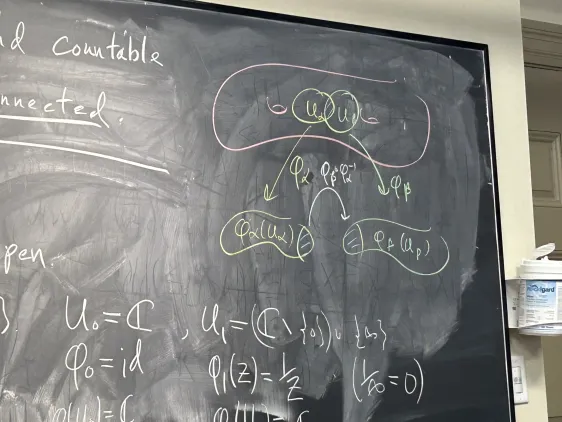
\includegraphics[width=0.5\textwidth]{Figures/cft-1.png}.\]
    \end{enumerate}
\end{example}

\begin{definition}
    A continuous map $f: X \to Y$ with $X, Y$ being Riemann surfaces is \textbf{holomorphic} if for all $\varphi: U \to \Cbb$ and $\psi: V \to \Cbb$ charts on $X$ and $Y$ respectively, then 
    \[\psi \circ f \circ \varphi^{-1} \text{ is holomorphic on $\varphi(f^{-1}(V) \cap U)$}.\]
\end{definition}

\begin{theorem}[Theorem]
    Let $f: X \to Y$ and $g: Y \to Z$ where $X, Y, Z$ Riemann surfaces. Then
    \[f, g \text{ is holomorphic } \implies g \circ f \text{ is holomorphic}.\]
    $f$ is a biholomorphism if $f$ is furthermore bijective and $f^{-1}$ is holomorphic.
\end{theorem}


\begin{example}[Different Choices of Charts can lead to different structures]
Note that different choices of charts on the same topological space $X$ could lead to different Riemann surfaces.\\

Take $\mathbb{D} \subseteq \Cbb$. Consider two different charts $\varphi: \mathbb{D} \to \Cbb$ by $\varphi(z) = z$ and $\psi: \mathbb{D} \to \Cbb, \psi(r e^{i\theta}) =  \frac{r}{1-r} e^{i\theta}$ (where we are taking the disk to the entire complex plane essentially). Certainly there are no biholomorphism between the two, otherwise it would imply that there's a non-constant holomorphic map from $\Cbb$ to $\mathbb{D}$, violating Liouville's theorem.    
\end{example}

\begin{theorem}[Theorem M]
    If $f: X \to Y$ is holomorphic and bijective, then its inverse $f^{-1}: Y \to X$ is also holomorphic.
\end{theorem}

\begin{proof}[Proof of Theorem M]
    Last semester, we proved that for $U^{open}, V^{open} \subseteq \Cbb$, if $f: U \to V$ is holomorphic and bijective, then $f^{-1}: V \to U$ is holomorphic. Here's a nice illustrative picture of what's going on:
    \[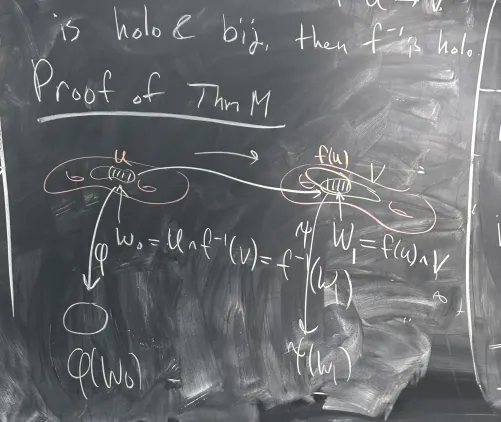
\includegraphics[width=0.5\textwidth]{Figures/cft-2.png},\]
    where the transition map from $\varphi(W_0)$ to $\psi(W_1)$ is bijective and holomorphic, so the inverse is holomorphic.
\end{proof}

\begin{example}[The Torus]
    Let $\Lambda = \Zbb + \Zbb \tau$ be a lattice in $\Cbb$, and let $X = \Cbb/\Lambda$ (in the sense that $\Lambda$ is a subgroup of $\Cbb$) and $\Lambda$ has a natural group action on $\Cbb$ by $(w, z) \in \Lambda \times \Cbb \to z + w$. We say that $z \sim z'$ if and only if there exists $w \in \Lambda$ such that $z' = z + w$.\\

    What are the charts of $X = \Cbb/\Lambda$? Suppose $U \subseteq \Cbb$ is open and $U \cap (U + w)$ is empty for all $w \in \Lambda$, then let $\Hat{U} = \{z + \Lambda\ |\ z \in U\} \subseteq X$. Then we can define $\varphi: \Hat{U} \to \Cbb$ defined by just $\varphi(z + \Lambda) = z$ for $z \in U$. The $\Hat{U}$ forms an open cover of the quotient space as we vary $U$ around satisfying the constraint.\\

    Finally, for any two charts $\varphi_0: \Hat{U_0} \to \Cbb$ and $\varphi_1: \Hat{U_1} \to \Cbb$, then $\varphi_1 \circ \varphi_0^{-1}$ is a translation map of the domain by an element of the lattice and is thus holomorphic.
\end{example}

\begin{example}[A Non-Hausdorff ``Riemann Surface"]
    Let $f(z) = z^2$ for $z \in A(r, 1)$ where $0 < r < 1$ and $A(r, 1)$ denotes the open annulus. Write $z_0 \sim z_1$ if there exists $k, \ell$ such that $f^k(z_0) = f^\ell(z_0)$ (the power here means composition). In other words, $f^k(z) = z^{2^k}$. Note that this is just the transitive closure of specifying $z \sim f(z) = z^2$.\\

    It turns out that $X = A(r, 1)/\sim$ satisfies all axioms of a Riemann Surface except being Hausdorff.
\end{example}

\newpage
\section{Lecture January 30th}

\textbf{Announcement:} Starting this Friday, you will be invited to submit 1 or 2 problems to the instructor from review, either from the notes or created by yourself! For making up questions yourself, the idea would be to answer questions that you have found over this course!!!! If it's from another source, you should absolutely cite it.

Recall from last time that - A Riemann surface $(X, \{\varphi_\alpha: U_\alpha \to \Cbb\})$ is a topological space $X$ with charts $\varphi_\alpha: U_\alpha \to \Cbb$ such that
\begin{itemize}
    \item $X$ is Hausdorff.
    \item The collection of $U_\alpha$ forms an open cover of $X$.
    \item For each $\alpha$, $\varphi_\alpha: U_\alpha \to \Cbb$ is a homeomorphic onto its image whose image is open in $\Cbb$.
    \item For all $\alpha$ and $\beta$, $\varphi_\beta \circ \varphi_\alpha^{-1}$ is holomorphic everywhere defined.
    \item $X$ is second countable (equivalently this follows from a deep theorem if $\{U_\alpha\}$ is countable).
    \item $X$ is connected. (otherwise $X$ is a complex $1$-manifold).
\end{itemize}

There are some slight \textbf{variations}:
\begin{itemize}
    \item If we let $\varphi_\beta \circ \varphi_{\alpha}^{-1}$ be smooth, then $X$ is a smooth surface.
    \item We can take $\varphi_\alpha: U_\alpha \to \Cbb^n$ and get a complex $n$-manifold (we do need to, however, define what a holomorphic map is between $\Cbb^n$).
    \item We can take $\varphi_\alpha: U_\alpha \to \Rbb^n$ with smooth overlaps to get a smooth $n$-manifold.
\end{itemize}

Note that Property 5 (2nd countable) is equivalent, on a manifold, to paracompact, which is equivalent to being metrizable. What's special about Riemann Surfaces are that Property $1, 2, 3, 4, 6$ actually implies Property $5$.

\subsection{Genus and Ends}

\begin{definition}
    An invertible linear map $T: \Rbb^n \to \Rbb^n$ is orientation-preserving if $\det(T) > 0$. It is orientation-reversing if $\det(T) < 0$.
\end{definition}

In particular, if $f: U \to \Cbb$ is holomorphic, then we can think of this a s a map $\hat{f}: U \subseteq \Rbb^2 \to \Rbb^2$. In this case, $D \hat{f}_z$ is orientation preserving because the derivative is of the form
\[\begin{pmatrix}
    u & v\\
    -v & u
\end{pmatrix},\]
by the Cauchy-Riemann equations, with determinant of the form $\det D\hat{f}_z = u^2 + v^2 > 0$ (as long as $f'(z) \neq 0$).\\

\begin{definition}
    A smooth $n$-manifold is \textbf{oriented} when given charts with $\det D_x(\varphi_\beta \circ \varphi_\alpha^{-1}) > 0$.
\end{definition}

In particular, this implies that
\begin{proposition}
    A Riemann Surface is always oriented.
\end{proposition}

First we restrict our attention to smooth surfaces. Let $X$ be a smooth orientable surface, then,

\begin{definition}
    The \textbf{genus} of $X$ is the maximal number of disjoint simple closed curves on $X$ that does not disconnect $X$ if removed. It is possible for a surface to have infinite genus. We should probably require the curves to be smooth, but the number turns out to be the same even if it's just continuous. A surface is said to be \textbf{planar} if it has genus $0$.
\end{definition}

Here we assume the following background results on smooth manifolds that are known already
\begin{theorem}
    Any compact surfaces have finite genus. Furthermore, any two connected compact (orientable) surfaces of genus $g$ are diffeomorphic.
\end{theorem}

Now we will also introduce the notion of \textbf{ends}. Let $X$ again be a smooth orientable surface.
\begin{definition}
If $K \subseteq L \subseteq X$, then we get an inclusion $X \setminus L \to X \setminus K$, and then this gives a well-defined map $i_{LK}: \operatorname{Comp}(X \setminus L) \to \operatorname{Comp}(X \setminus K)$ where $\operatorname{Comp}$ refers to connected components (thought of as discrete topological spaces).\\

Then we define $\mathcal{E}(X)$ (``space of ends of $X$") be the inverse limit
\[\varprojlim i_{KL}\]
indexed over all compact subsets $K \subseteq X$ in the following sense:
% https://q.uiver.app/#q=WzAsNCxbMSwxLCJcXG9wZXJhdG9ybmFtZXtDb21wfShYIFxcc2V0bWludXMgTCkiXSxbMSwyLCJcXG9wZXJhdG9ybmFtZXtDb21wfShYIFxcc2V0bWludXMgSykiXSxbMCwwLCJcXG1hdGhjYWx7RX0oWCkiXSxbMSwwLCIuLi4iXSxbMiwwXSxbMiwxXSxbMCwxXSxbMiwzXSxbMywwXV0=
\[\begin{tikzcd}
	{\mathcal{E}(X)} & {...} \\
	& {\operatorname{Comp}(X \setminus L)} \\
	& {\operatorname{Comp}(X \setminus K)}
	\arrow[from=1-1, to=2-2]
	\arrow[from=1-1, to=3-2]
	\arrow[from=2-2, to=3-2]
	\arrow[from=1-1, to=1-2]
	\arrow[from=1-2, to=2-2]
\end{tikzcd}\]
Here's an alternative more concrete characterization - for each $e \in \mathcal{E}(X)$ and compact $K \subseteq X$, we get $e_K \in \operatorname{Comp}(X \setminus K)$ (by the map given in universal property). Hence we can think of $e$ as a choice of component in $X \setminus K$. Furthermore, this satisfies
\[i_{LK}(e_L) = e_K.\]
So it's the set of choices of components that are consistent with respect to inclusion $X - L \to X - K$. The base for topology $B$ of $\mathcal{E}(X)$ in this case is
\[\Hat{U} = \{e \in \mathcal{E}(X)\ |\ e_K = U\},\]
where $U \in \operatorname{Comp}(X \setminus K)$.\\

$\mathcal{E}(X)$ is roughly ``ways you can go to $\infty$ in $X$". The concept works intelligently in locally compact spaces.
\end{definition}

\begin{example}
    Here are some example of ends,
    \begin{itemize}
        \item  Note that if $X$ is compact, then $\mathcal{E}(X)$ is empty.
        \item For an infinite cylinder $S^1 \times \Rbb$, there are two ends at infinity.
        \item This surface $X$ actually only has one end:
        \[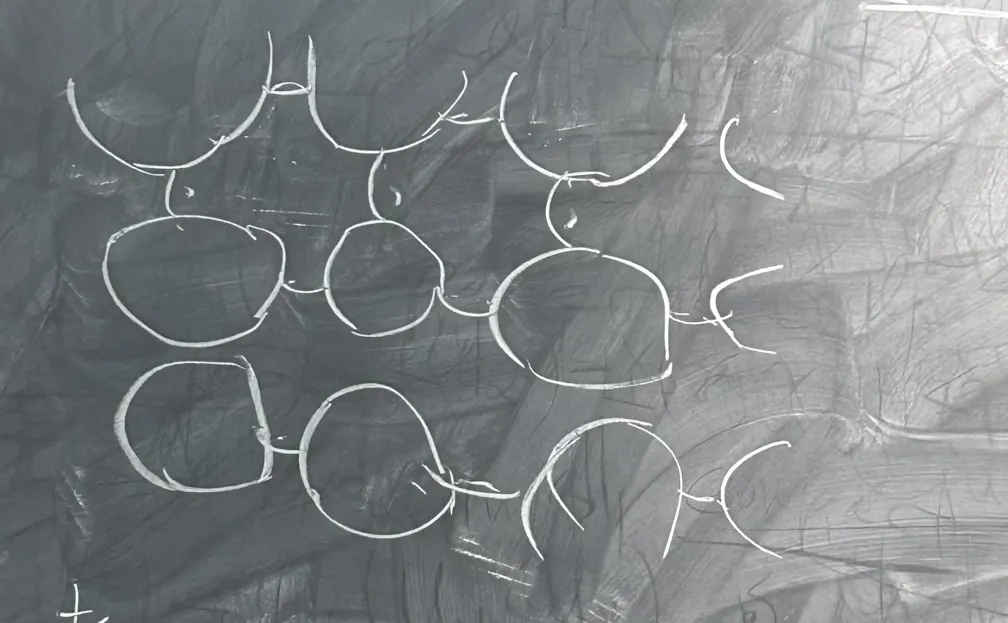
\includegraphics[width=0.6\textwidth]{Figures/lec2-1.png}\]
        This is because every way to go to infinity is equivalent to the complement of $X \cap \overline{B}_{R}(0)$ as $R$ gets larger.
        \item $\Cbb \setminus \{\text{n points}\}$ has $n+1$ ends. $\Cbb$ itself has $1$ end at infinity.
    \end{itemize}
\end{example}

\begin{exercise}
    If $X$ is a surface and $A \subseteq X$ is compact, $\mathcal{E}(X \setminus A) \equiv \mathcal{E}(X) \sqcup \operatorname{Comp}(A)$ (canonically homeomorphic).
\end{exercise}

\begin{exercise}
    If $X$ is a surface, then $X \sqcup \mathcal{E}(X)$ is compact, the topology here is $U = U_X \cup \{\Hat{U} \subseteq \mathcal{E}(X) \text{ union } U \subseteq X, \text{ for each } U \in \operatorname{Comp}(X \setminus K)\}$. Furthermore, $\mathcal{E}(X) \subseteq X \sqcup \mathcal{E}(X)$ is closed under the given topology (this sort of follows immediately because the definition requires any open subset of $X$ to be open in the disjoint union, including $X$ itself).
\end{exercise}

Note that $X_n \to e$ for sequence $X_n \in X$ and $e \in \mathcal{E}(X)$ if and only if for all compact $K \subseteq X$, $X_n \in e_K \in \operatorname{Comp}(X \setminus K)$ for all large $n$.

\begin{definition}
    An end is \textbf{planar} if has a \textbf{planar} (genus zero) neighborhood (take a compact set, see which component the end takes in the complement). Note that the set of planar ends $\mathcal{P}(X)$ are open.
\end{definition}

For example, this has two ends,
\[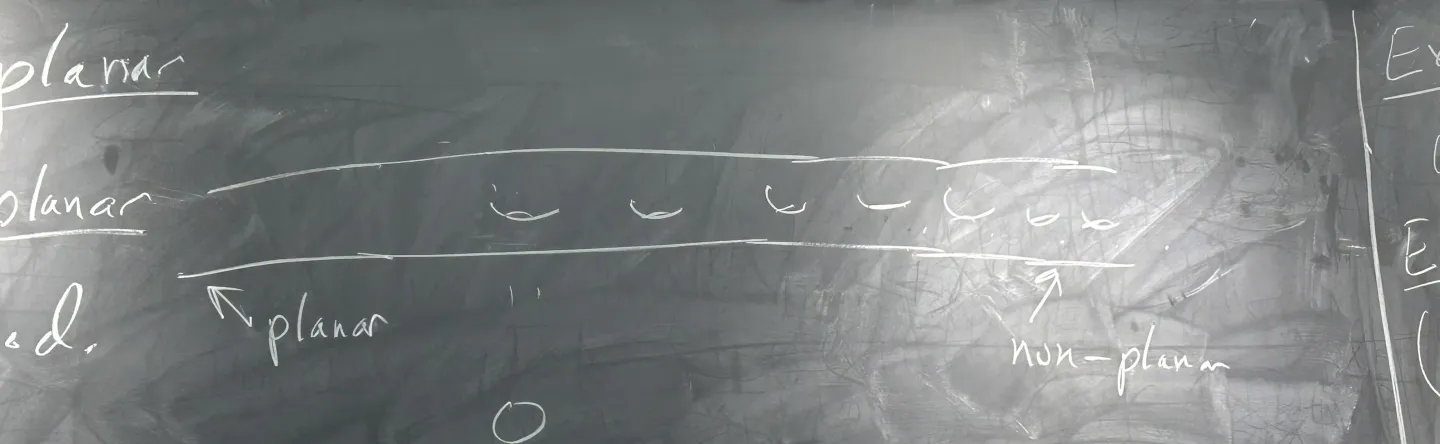
\includegraphics[width=0.6\textwidth]{Figures/lec2-2.png}\]
The left side is planar. The right side is not planar.\\

Given $X$, we get the genus $g(X) \subseteq \Nbb \cup \{\infty\}$, ends $\mathcal{E}(X)$, and $\mathcal{P}(X) \subseteq \mathcal{E}(X)$ open. The amazing theorem we get is that
\begin{theorem}
    For all triples $(g, \mathcal{E}, \mathcal{P})$ with $\mathcal{E}$ totally disconnected, metrizable, and compact, $\mathcal{P}(X) \subseteq \mathcal{E}(X)$ open with $P = \mathcal{E}$ if $g < \infty$. Then there exists a surface $X$ with these invariants unique up to diffeomorphism. 
\end{theorem}

\newpage
\section{Lecture February 1st}

\subsection{Pullback of Riemann Surface Structure}

Let $f: X \to Y$ be a continuous map, we say it's a local homeomorphism if for all $x \in X$, there exists $U \subseteq X$ containing $x$ and $V \subseteq Y$ (U, V open), such that $f$ is a homeomorphism of $U$ onto $V$.

\begin{theorem}
Suppose $Y$ is a Riemann Surface, and $X$ is connected and Hausdorff, and $f: X \to Y$ is a local homeomorphism, then there exists a unique Riemannian surface structures on $X$ such that $f: X \to Y$ is then holomorphic.\\

By the existence of Riemann surface structure, we mean a collection of charts $\varphi_\alpha: U_\alpha \to \Cbb$ on $X$.\\

By the uniqueness of Riemann surface structure, we mean that the overlap/transition function on the combination of all charts are still holomorphic (equivalently, they are contained in the same maximal atlas). More equivalently, let $\sigma$ and $\tau$ be two Riemannian surface structures on $X$, then the identity map
\[(X, \sigma) \to (X, \tau)\]
is a holomorphic map.
\end{theorem}

\begin{remark}
    In particular, any covering space $\rho: X \to Y$ will satisfy the description above, hence covering spaces of Riemann surfaces have unique Riemann surface structures.
\end{remark}

\begin{remark}
    Given $X$ and a Riemannian surface structure $\sigma$ with charts $\varphi_\alpha: U_\alpha \to \Cbb$. Let $\operatorname{conj}: \Cbb \to \Cbb$ be the complex conjugation map, then define charts $\psi_\alpha = \operatorname{conj} \circ \varphi_\alpha$, this gives a Riemannian surface structure $\tau$ on $X$. In this case, the identity map
    \[id: (X, \sigma) \to (X, \tau)\]
    is \textbf{anti-holomorphic}.
\end{remark}

\begin{proof}[Proof of the Theorem]
    Let $x \in X$, let $(U, V)$ be the pair of open sets in $X$ and $Y$ respectively under the local homeomorphism hypothesis. Without loss of generality (taking intersection with charts of $Y$), we can assume that there's a chart $\psi: V \to \Cbb$, then we define a map $\phi: U \to \Cbb$ such that
    \[\phi = \psi \circ f,\]
    then it's a routine exercise to verify that the charts on $X$ gives it a Riemannian surface structure (since $X$ is already connected and Hausdorff), and that $f$ is holomorphic.\\
    
    The only issue with this proof is that we DID NOT assume that $X$ is second countable. Now it is a very deep theorem (as we said before) that all the other conditions imply that $X$ is second countable, but that's a very big result.\\

    For uniqueness, use the fact that $f$ is a local homeomorphism to try to construct an identity map on $X$ that is holomorphic.
\end{proof}

\begin{exercise}[Student is encouraged to do this...]
    Prove $X$ has holomorphic overlaps and $f: X \to Y$ is holomorphic.
\end{exercise}

\begin{exercise}
    Assume that $X$ is 2nd countable, or does it follow?
\end{exercise}

\subsection{Local Branched Cover of Oriented Surfaces}

\textbf{Motivation:} Consider the map $z \mapsto z^n$ on the unit disk $\mathbb{D} \subseteq \Cbb$, then this gives an degree $n$ covering map $\mathbb{D} - \{0\} \to \mathbb{D} - \{0\}$.

\begin{definition}
    Between oriented surfaces, $f: X \to Y$ (continuous map) is a branched cover if for all $x$, there exists open $U \subseteq X$ containing $x$, $V \subseteq Y$ containing $f(x)$ (both $U$ and $V$ are topological disks) such that
    \begin{itemize}
        \item $f: U \setminus \{x\} \to Y \setminus \{f(x)\}$  is a proper local homeomorphism. (note that if the degree is $n < \infty$, then it is actually topologically equivalent to what we said in the Motivation).
    \end{itemize}
\end{definition}

There's a brief lemma we glossed over in the definition above we need to justify:
\begin{lemma}[Lemma B]
    Let $U$ and $V$ be topological disks and $f: U \to V$ is continuous. Suppose f restricted to $U \setminus \{x\} \to V \setminus \{f(x)\}$ is a proper local homeomorphism (which is a finite sheeted covering map, with degree say $n$), then there exists $h_U, h_V$ homeomorphisms to the disk such that the diagram commutes:
    % https://q.uiver.app/#q=WzAsNCxbMCwwLCJVIl0sWzIsMCwiViJdLFswLDIsIlxcbWF0aGJie0R9Il0sWzIsMiwiXFxtYXRoYmJ7RH0iXSxbMCwyLCJoX1UiXSxbMCwxLCJmIl0sWzEsMywiaF9WIiwyXSxbMiwzLCJ6IFxcbWFwc3RvIHpebiJdXQ==
\[\begin{tikzcd}
	U && V \\
	\\
	{\mathbb{D}} && {\mathbb{D}}
	\arrow["{h_U}", from=1-1, to=3-1]
	\arrow["f", from=1-1, to=1-3]
	\arrow["{h_V}"', from=1-3, to=3-3]
	\arrow["{z \mapsto z^n}", from=3-1, to=3-3]
\end{tikzcd}\]
\end{lemma}

Here's another topological fact
\begin{exercise}
    Let $g: X \to Y$ be a proper local homeomorphism between surfaces, then $g$ is a finite-sheeted cover.
\end{exercise}

\begin{proof}[Proof of Lemma B]
    Take $h_V$ with $h_V(f(x)) = 0$ (by a Mobius transformation), then we lift $h_V \circ f$ by $z \mapsto z^n$ where $n = \operatorname{deg}(f)$ on $U - \{x\}$. So $h_V \circ f$ and $(z \mapsto z^n)$ are both covering maps that have the same image (in terms of fundamental groups), so from covering space theory we can lift $h_V \circ f$ to give a covering map $h_U: U \to \mathbb{D}$ that makes the diagram commute:
    \[\begin{tikzcd}
	U && V \\
	\\
	{\mathbb{D}} && {\mathbb{D}}
	\arrow["{h_U}", from=1-1, to=3-1]
	\arrow["f", from=1-1, to=1-3]
	\arrow["{h_V}"', from=1-3, to=3-3]
	\arrow["{z \mapsto z^n}", from=3-1, to=3-3]
\end{tikzcd},\]
then one can check that $h_U$ is a homeomorphism.\\

\textbf{Exercise:} Fill in the details of this proof.
\end{proof}

Now we have reached a new theorem:
\begin{theorem}
    If $Y$ is a Riemann surface and $f: X \to Y$ is a local branched cover, and $X$ is connected and Hausdorff (and second countable), then there exists an unique Riemann surface structure on $X$ such that $f: X \to Y$ is holomorphic.
\end{theorem}

\begin{proof}
    First observe that the set $B \subseteq X$ of \textbf{branched points} (the points where $f$ is not a local homeomorphism) is discrete, then $f: X \setminus B \to Y$ is a local homeomorphism. Since $B$ is discrete, $X \setminus B$ is still RS, and the previous theorem tells us that there exists an unique Riemann surface structure on $X \setminus B$.\\

    For each $x \in B$, we can use $h_{U}: \hat{U} \to \mathbb{D}$ where given by Lemma B, where $h_V: \hat{V} \to \mathbb{D}$ is a holomorphic homeomorphism (after possible intersection with the charts already given and taking pre-images - essentially we are shrinking $U, V$ until we get into holomorphic charts).\\

    Here's an illustrative diagram indicating roughly what's happening in the discussion above:
\[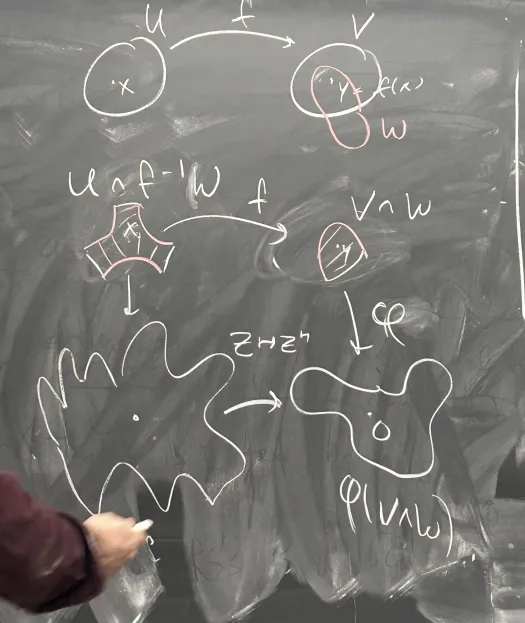
\includegraphics[width=0.4\textwidth]{Figures/lec3-1.png}\]

    The branched points are discrete because each point is isolated because $f$ is supposed to be a local homeomorphism on $N - \{p\}$ in a neighborhood $N$ containing the branch point $p$.\\

    \textbf{Exercise: } Verify holomorphic and explain $\hat{U}$.\\

    For uniqueness of the Riemannian Surface structure, given two structures near $X$, \underline{lift} $f$ near $X$ \underline{by} $f$ to get that the identity map of $U \setminus \{x\}$ is holomorphic, and by the Riemann removable singularity theorem, it is holomorphic on $U$.
\end{proof}

In fact, there's another theorem:
\begin{theorem}
    Every non-constant holomorphic map of Riemann surfaces is a local branched cover.
\end{theorem}

\subsection{Building Riemann Surfaces}
So far, we haven't built that much Riemann Surfaces yet, but we can now try to build some with the theorems given.\\

Suppose $E \subseteq Y$ is a discrete subset of a Riemann Surface (sometimes called the branched values), then take $H$ a subgroup of $\pi_1(Y \setminus E)$ of finite index $n$. Galois correspondence tells us that there exists a degree $n$ covering map from $g: X' \to Y \setminus E$. Near each $y \in E$, we get this finite covering map $g: U' \to V - \{y\}$, where $U', V$ are appropriately small disks.\\

\textbf{Claim: } We can fill in each $U'$ to make $U$ such that $g: U \to V$ is a local branched cover (and we also complete $X'$ to $X$), and then $g: X \to Y$ is a (global) branched cover.\\

\textbf{Note: } A global branched cover have several definitions that agree on a finite sheeted cover, but we will settle to one of them in the case of finite sheeted cover:
\begin{itemize}
    \item For all $y \in Y$, there exists $V \equiv V_y \subseteq Y$ containing $y$ such that $g$ on each component $U_i$ of $g^{-1}(V)$ gives:
    \item There exists $x_i \in U_i$ with $g^{-1}(y) \cap \{U_i\} = \{x_i\}$, and $g: U_i - \{x_i\} \to V - \{y\}$ is a proper local homeomorphism.
    \item See the following illustrate picture
\[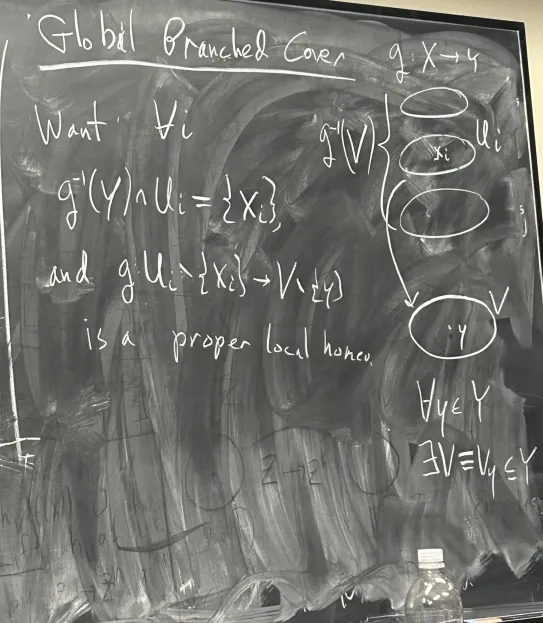
\includegraphics[width=0.4\textwidth]{Figures/lec3-2.png}\]
\end{itemize}

\begin{question}
    How can we fill $U'$ to $U$?
\end{question}

Well, locally we have that $U, V$ is homeomorphic to $\mathbb{D} \setminus \{0\}$ and the map behaves like $z \mapsto z^n$, we want to then continuously extend the homeomorphism to the origin and then lift that to $\mathcal{E}(U')$ to be added to $U'$. Even without considering ends, we could do something like
\[X' \sqcup \mathbb{D} / h_{U'}\]
via an appropriate quotient map. Please see the following illustrative picture:
\[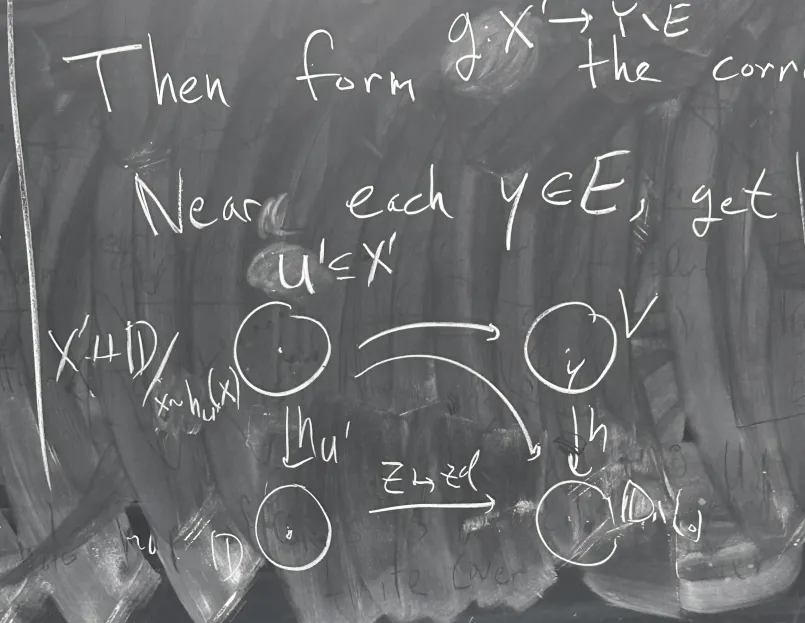
\includegraphics[width=0.5\textwidth]{Figures/lec3-3.png}\]

\newpage
\section{Lecture February 6th}

\subsection{Possibly Large Riemann Surfaces}

\begin{definition}
    A \textbf{possibly large} Riemann Surface $X$ is one where $X$ satisfies all axioms except (possibly) 2nd countable. Of course, by Rado's Theorem, we will see later that all possibly large Riemann surfaces are second countable, but we would like to work without this assumption yet.
\end{definition}

This definition is motivated because we actually figured out the questions bugging us last time:
\begin{theorem}[Poincare-Volterra Theorem]
    Suppose $f: X \to Y$ is a local homeomorphism (or local branched cover) of possibly large surfaces, and $Y$ is second countable, then $X$ is second countable.
\end{theorem}

\begin{remark}
    The theorem above is not Poincare-Volterra Theorem in its full generality but rather only a special case.
\end{remark}

\begin{proof}
The proof is divided into the following steps:
\begin{enumerate}
    \item As an exercise, we note that a Riemann surface is second countable if and only if it admits a countable cover by charts (that in fact forms a basis).
    \item Since $Y$ is second countable, let $W = \{W_i\}$ be a countable cover of $Y$ of connected charts.
    \item Let $\mathcal{V} = \{V \subseteq X\ |\ f(V) \in W \text{ and } f: V \to f(V) \text{ is a homeomorphism}\}$. We see that $\mathcal{V}$ is actually a base for topology on $X$, the idea is that - given any $x \in X$, we can find a neighborhood of $x$ that's mapped homeomorphically into $Y$, we then find a neighborhood around the image given by $W_i$ that pullback to a base for topology.
    \item \textbf{Claim: } $\mathcal{V}$ is a countable set. B.  For all $V \in \mathcal{V}$, the set $\{V' \in \mathcal{V}\ |\ V \cap V' \neq \emptyset\}$ (where $V$ is fixed) is countable. Indeed, consider the function $f$ restricted to each neighborhoods in the set $\{V' \in \mathcal{V}\ |\ V \cap V' \neq \emptyset\}$ is countable-to-1. \mattie{what}
    \item C. Choose $V_0 \in \mathcal{V}$, let $\mathcal{V}_0 = \{V_0\}$, and generally we construct
    \[\mathcal{V}_{k+1} = \{V \in \mathcal{V}\ |\ \exists V' \in \mathcal{V}_k \text{ such that } V \cap V' \neq \emptyset\}.\]
    The picture to have in mind is everything you can reach in $k+1$ steps:
    \[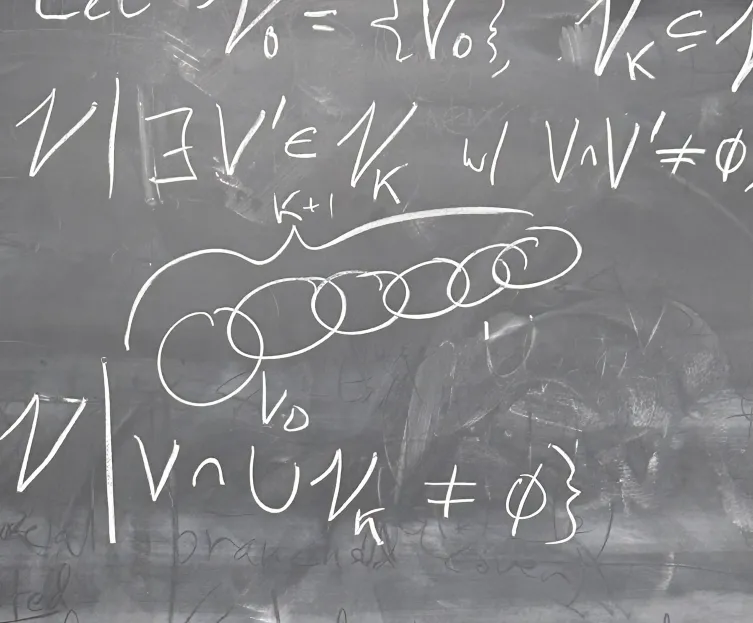
\includegraphics[width=0.5\textwidth]{Figures/lec4-1.png}\]
    Equivalently $V_{k+1}$ is the set
    \[\mathcal{V}_{k+1} = \{V \in \mathcal{V}\ |\ V \cap \bigcup_{i = 1}^k \mathcal{V}_k \neq \emptyset\}\]
    \item Then $\mathcal{V}_k$ is countable by B and induction. Hence we have that
    \[\mathcal{V}_\infty = \bigcup_{k = 0}^\infty \mathcal{V}_k\]
    is countable. Note that we haven't used connectedness yet.
    \item D. We claim that the union $\bigcup_{V \in \mathcal{V}_\infty} V = X$ (\textbf{Notaton:} We use $\bigcup \mathcal{V}_\infty$ to denote the union $\bigcup_{V \in \mathcal{V}_\infty} V$, this is a notation from set theory that is adopted here.) 
    \begin{proof}[Proof of D]
        If this is not the case, then $\mathcal{V}_\infty \subsetneq \mathcal{V}$ and $X \setminus \bigcup \mathcal{V}_\infty = \bigcup (\mathcal{V} - \mathcal{V}_\infty)$. Then $\bigcup \mathcal{V}_\infty$ and $X \setminus \bigcup \mathcal{V}_\infty$ are both open disjoint non-empty sets, so $X$ would be disconnected!
    \end{proof}
    \item Thus $\bigcup_{V \in \mathcal{V}_\infty} V = X$ so $X$ can be covered by countable neighborhoods.
\end{enumerate}
\end{proof}

Last time, we were also constructing examples of Riemann surfaces.
\begin{example}
    Let $E \subseteq \hat{\Cbb}$ be finite, let $H \setminus \pi_1(\hat{\Cbb} \setminus E)$ be a subgroup of finite index. Then we get a finite-sheeted cover $\hat{X}$ of $\hat{\Cbb} \setminus E$ that can be filled into a covering map $\pi: X \to \hat{\Cbb}$ with $\pi: X \to \hat{\Cbb}$ with $\pi$ as a branched cover and $X$ is compact.\\

    To make this notion rigorous, we should develop some more discussion about ends. Indeed, for a general surface $X$, for all $e \in \mathcal{E}(X)$, there exists $\alpha: [0, 1) \to X$ with $\lim_{t \to 1} \alpha(t) = e$, with the properties:
    \begin{itemize}
        \item Every proper path in $X$ limits to a unique end (proper here means $\alpha^{-1}(K)$ is compact for all compact $K \in X$). 
        \item Properly paths are properly homotopic implies they limit to the same end. By \textbf{properly homotopic}, we mean that for $\alpha_0, \alpha_1: [0, 1) \to X$, then a proper homotopy is - $\alpha: [0, 1] \times [0, 1)$ where we write $\alpha(s, t) = \alpha_s(t)$ where $\alpha$ is proper. (NOTE THAT WE DO NOT REQUIRE $\alpha$ to fix end points). 
        \item If the ends are isolated, the converse is also true (probably, the instructor's a bit unsure).
    \end{itemize}
    We could use these discussion of proper paths to do the extension mentioned in the example.
\end{example}

\begin{remark}
    There is a discussion of everything talked about here for review in the first 5 sections of Forster.
\end{remark}

\subsection{Hyperelliptic Covers}

\begin{proposition}
Now suppose that $F \subseteq \widehat{\Cbb}$ has even cardinality, then there exists a unique ($X$, $g: X \to \widehat{\Cbb}$) such that $g$ is a \textbf{holomorphic degree $2$ branched cover}, branched exactly over the points of $F$.    
\end{proposition}

This is what's called a \textbf{hyperelliptic cover}. This theorem essentially classifies all degree $2$ cover over $\widehat{\Cbb)$ based on its branch values.

\begin{proof}
\begin{enumerate}
    \item What is $\pi_1(\widehat{\Cbb} \setminus F)$? It is the free group of rank $2k - 1$. More geometrically it is also the group
    \[\langle g_1, ..., g_{2k}\ |\ g_1 ... g_{2k} = 1\rangle\]
    \item What are the subgroup $H$ of $\pi_1(\widehat{\Cbb} \setminus F)$ with index $2$? We first note all index $2$ subgroups are normal, the only order $2$ group is $\Zbb/2\Zbb$. In other words, all index $2$ normal subgroups are kernels of the homomorphism
    \[h: F_{2k - 1} \to \Zbb/(2\Zbb)\]
    How many such homomorphisms are there? Well, there are exactly $2^{2k-1}$ of them, based on what they send the generators to.
    \item Given some $h: F_{2k-1} \to \Zbb/2\Zbb$, what are the points that $h$ is branched over? Indeed, it's exactly the $z_i = h(g_i) = 1 \in \Zbb/2\Zbb$.
    \item What about the point at infinity? Topologically this happens, when we have a curve over the point at infinity. This happens when $h(g_i) = 1$ for all $i$.
    \item This is because $h(g_{2k}) = \sum_{i = 1}^{2k-1} h(g_i)$
    \item Therefore, there's only one unique branched cover with the constraint
    \[h(g_1) = ... = h(g_{2k-1}) = 1\]
\end{enumerate}
Note: To be branched over a point means - if you start with a point - it means one of these $n_i$ has to be greater than $1$
\end{proof}

\subsection{Geometric Realization of the Hyperelliptic Cover}
Here's also a more geometric perspective on what is happening:\\

Specifically, suppose that $E \subseteq \widehat{\Cbb}$ has even cardinality, and let ($X$, $g: X \to \widehat{\Cbb}$) be the branched double cover over $\widehat{\Cbb}$ branched at $E$. Note that we never explicitly spelled out what the hyper-elliptic cover $X$ is look.

Here we give an explicit construction of what $X$ is. Indeed, $X$ maybe constructed explicitly as follows.\\

Let $|E| = 2n$ for $n \geq 1$, and let $Y$ be the genus $n-1$ surface as follows:
\[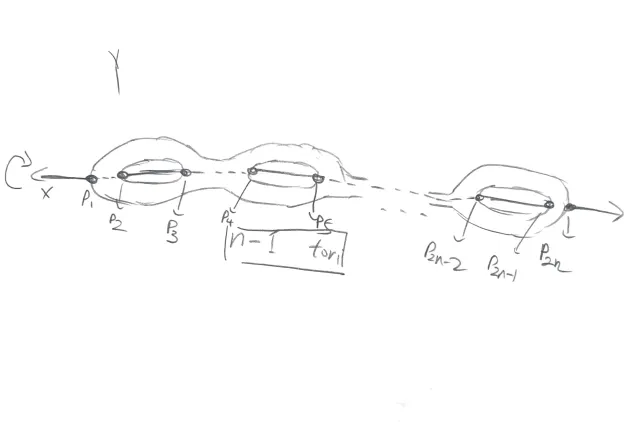
\includegraphics[width=0.6\textwidth]{Figures/hyper.png}\]
Although the diagram is not perfect, you should think of the $x$-axis as straight and $Y$ as being symmetric with respect to the $x$-axis.\\

Now consider the group action $\Zbb/2\Zbb$ on $Y$ given by rotating along the $x$-axis by $180$ degrees. Then this action will have orbit of size $2$ for every point on $Y$ except for $p_1, ...., p_{2n}$ labeled. The set $\{p_1, ..., p_{2n}\}$ are the fixed point of this group action (ie. they have orbit one).\\

Hence, we obtain a degree $2$ branched cover $p: Y \to Y/G$ branched at exactly $\{p_1, ..., p_{2n}\}$. Furthermore, if you examine what $Y/G$ is, it would be $\hat{\Cbb}$. One could deduce this from more rigorous arguments but just investigate what points gets glued to which, the resulting surface in the quotient will have genus $0$.\\

Thus, we have that the hyperelliptic double covers discussed in classes are homeomorphic to a genus $n-1$ surface. This also shows that we can give a Riemann surface structure of any closed surface of genus $g$ by considering this branched cover.



\newpage
\section{Lecture February 8th}

\textbf{Office Hour: } Thursday 4 - 5 pm (or by appointment).\\

From last time, for the hyperelliptic cover. Consider $E \subseteq \hat{\Cbb}$ be a finite set of even points and $\infty \in E$. Write $\hat{E} = E - \infty$, then consider the map
\[q: \pi_1(\Cbb \setminus E') \to \Zbb/2\Zbb\]
by sending $\alpha_i \to 1$ where each $\alpha_i$ is a generator of $\pi_1(\Cbb \setminus E') \cong F^{2k-1}$ (free group on odd many generators).\\

 This gives an index $2$ subgroup $H = \ker(q)$ in $\pi_1(\Cbb \setminus E)$. If any of the $\alpha_i$ has $h(\alpha_i) = 0$, then it means that when we loop around the puncture given by $\alpha_i$, we are not switching branches, so the covering space is not branched over $\alpha_i$. Since $|E'|$ is odd, then the sum of all $q(\alpha_i)$ is $1$ modulo $2$ (which guarantees that it's branched over infinity - this is because a loop around infinity is freely homotopic to a loop going around all the points $\alpha_i$'s, and we ignore minus signs because it is mod $2$).

 \subsection{Riemann Surfaces and Analytic Continuations}

 \begin{definition}
     If $f_0: U_0 \to \Cbb$ and $f_1: U_1 \to \Cbb$ are holomorphic ($U_0, U_1$ are open), and $z \in U_0 \cap U_1$, then we say that $[f_0, z] = [f_1, z]$ (the \textbf{germ} of $f_0$ at $z$ if equal to the \textbf{germ} of $f_1$ at $z$) if there exists open $V \subseteq U_0 \cap U_1$ containing $z$ such that
     \[f_0|_V = f_1|_V.\]
     Note that by the identity theorem, this is equivalent to $f_0 = f_1$ on the component $W$ of $U_0 \cap U_1$ containing $z$.\\
     
     For $f: U \to \Cbb$ be holomorphic, we let $[f, U] = \{[f, z]\ |\ z \in U\}$ up to the equivalence class with the identification given above.\\

     From here we define $\mathcal{G}(\Cbb, \Cbb)$ (or more generally $\mathcal{G}(X, \Cbb)$ or $\mathcal{G}(X, Y)$ for Riemann surfaces) as
     \[\mathcal{G}(X, Y) = \{[f, x]\ |\ x \in U, f: U \subseteq X \to Y \text{ is holomorphic}\}.\]
     In this case $\{[f, U]\}$ is a base for the topology of $\mathcal{G}(X, Y)$.
 \end{definition}

In the last semester, we proved the following theorem
 \begin{theorem}[Fall 2023, Theorem 1]
     The space $\mathcal{G} \coloneqq \mathcal{G}(X, \Cbb)$ is Hausdorff. Furthermore, every component $Q$ of $\mathcal{G}$ has canonical local homeomorphism (projection by $[f, z] \to z$) $\pi: Q \to X$. (In fact, the projection $\pi: \mathcal{G} \to X$ is a local homeomorphism)\\
     
     Furthermore, our result from last week shows that each $Q$ has an unique Riemann surface structure as $\pi$ is a local homeomorphism making $\pi$ holomorphic. The very obvious Riemann surface structure is that $[f, U] \mapsto U$.
 \end{theorem}

 \begin{remark}
     $\mathcal{G}$ itself is not second countable.
 \end{remark}

We also had a second theorem.
\begin{theorem}[Fall 2023, Theorem 2, Monodromy Theorem]
    We are working in $\mathcal{G} = \mathcal{G}(X, \Cbb)$. If $\gamma_0, \gamma_1: I = [0, b] \to X$ (where $X$ is a Riemann Surface) are homotopic rel end points by a homotopy $\gamma_t: I \to X$ such that each $\gamma_t$ has a lift to $\mathcal{G}$ starting at $z_0$ ($\gamma_t(0) = z_0$ for all $t$).\\

    Then $\gamma_t(b)$ is constant independent of $t$. \mattie{explain wording}
\end{theorem}

\begin{question}
    When can we analytically continue along $\gamma$?
\end{question}

\begin{example}
    Suppose $f: \Cbb \to \Cbb$ is holomorphic, and $g: U \to \Cbb$ is a branch of $f^{-1}$ near $z_0 \in U$ (which just means that $g$ is holomorphic and $f \circ g = id$ on $U$). For instance, when $f(z) = e^z$, we could take $g(w) = \operatorname{Log} w$ to be on $\Cbb \setminus (-\infty, 0)$ where we take $-\pi < \operatorname{Im}(g(w)) < +\pi$.

    \begin{question}
        Take $\gamma: [0, b] \to \Cbb$ with $\gamma(0) = z_0$, when we can we analytically continue $g$ along $\gamma$?
    \end{question}

    In the special case with $f(z) = e^z$ as before. Let's pick $z_0 = 1$, so $g(z_0) = 0$. If the path we take crosses $(-\infty, 0)$, we would want to path to go out of $[-\pi, \pi]$.
    \[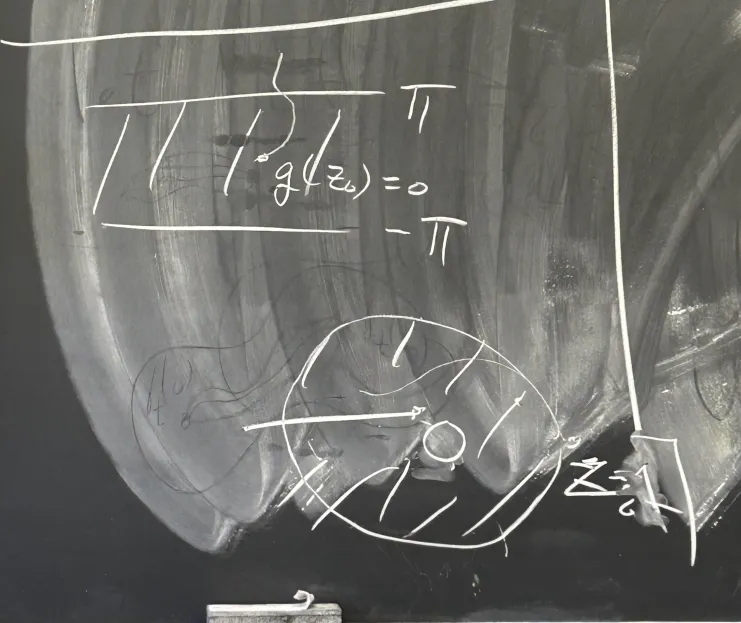
\includegraphics[width=0.5\textwidth]{Figures/lec5-1.png}\]
    More formally, $z \mapsto e^z: \Cbb \to \Cbb^*$ is a covering map, so we know that topologically we could always lift a path.
\end{example}

\begin{question}
    Another example is to consider $\sin: \Cbb \to \Cbb$, when can we analytically continue branch of $\sin^{-1}$?
\end{question}

Here's the general theory that may be able to help.
\begin{theorem}
    Suppose $f: U \subseteq \Cbb \to \Cbb$ is holomorphic and $\gamma: [0, b] \to \Cbb$. We can analytically continue along $\gamma$ starting from $g$ a branch of $f^{-1}$ near $\gamma(0) \in f(U)$ unless:
    \begin{itemize}
        \item There exist $0 \leq c \leq b$ such that $[0, c)$ is maximal interval for analytic continuation.
        \item And either (1) $g(\gamma(t)) \to $ critical point of $f$ or (2) $g(\gamma(t)) \to \infty$ in $U$ as $t \to c$ (we don't mean literal infinity, but to an end of $U$).
    \end{itemize}
\end{theorem}

Here's an example of how $(1)$ could occur:
\begin{example}
    Take $f(z) = z^2$ and it's ambiguous where lift the path past $\gamma(c) = 0$,
    \[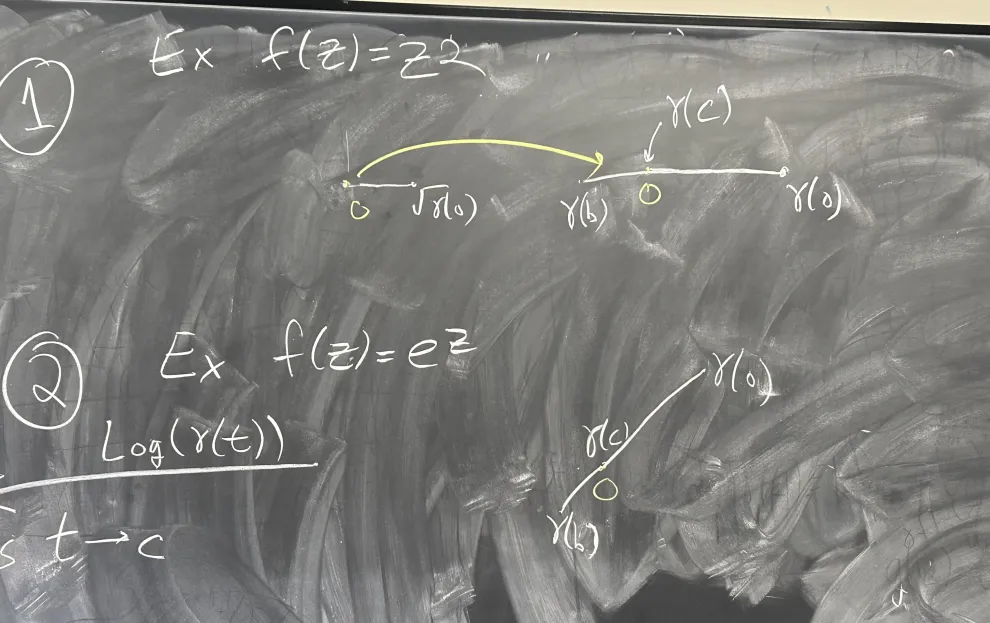
\includegraphics[width=0.5\textwidth]{Figures/lec5-2.png}\]
    This is because you are hitting a point where you don't really have a local inverse.
\end{example}

Here's an example of how $(2)$ could occur:
\begin{example}
    Take $f(z) = e^z$, then it's still ambiguous what happens at $\gamma(c) = 0$ (see the previous picture for a figure of this as well), because $\operatorname{Log}(\gamma(t))$ blows up at $t = c$. The caveat however is that $e^z$ will never hit $0$ for any value $z \in \Cbb$, so maybe this example is not that good, but it is going to infinity in the sense that it's going to an end.\\

    For clarity, let's consider the following example instead:
    \[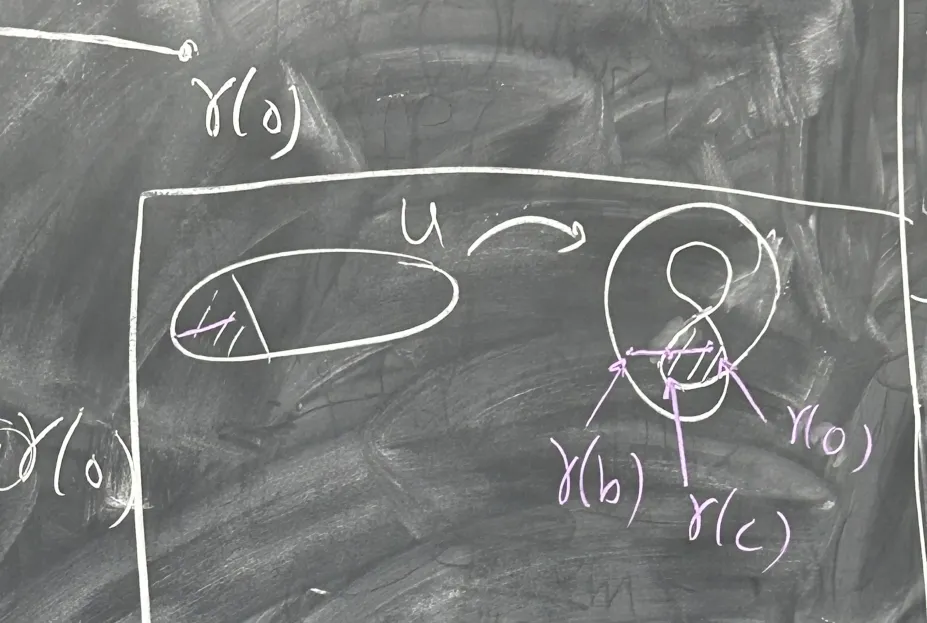
\includegraphics[width=0.5\textwidth]{Figures/lec5-3.png}\]
    where the path is also leaving $U$.
\end{example}

\begin{question}
    But what if we analytically continue $f$ itself outside of $U$? So, we really want to think of $U$ as an independent Riemann surface instead or assume it's the maximal analytic domain of $f$.
\end{question}

\textbf{NOTATION CHANGE:} Let's just assume $U = X$ is a Riemann surface instead.\\

\begin{definition}
    $\gamma(c)$ in Condition (1) is called a branch value or critical value. $\gamma(c)$ in Condition 2 is called an ``asymptotic value".
\end{definition}

\newpage
\section{Lecture Ferbuary 15th}

Recall from last lecture, we defined that
\begin{definition}
    Suppose $f: X \to Y$ is holomorphic, then $q \in Y$ is an \textbf{asymptotic value} of $f$ if there exists $\alpha: [0, \infty)$ continuous and proper, such that
    \[\lim_{t \to \infty} f(\alpha(t)) = q.\]
\end{definition}

\begin{example}
    Consider the function $f: \Cbb \to \Cbb$ given by $f(x) = e^{x}$, then we observe that $\lim_{t \to \infty} f(-t) = 0$. Note that $f$ has no continuous extension to $\hat{\Cbb}$, indeed if there is, then the extension $\hat{f}: \Cbb \cup \{\infty\} \to \Cbb \cup \{\infty\}$ would be a rational function. However, the function would have an essential singularity at $\infty$, which is a contradiction.
\end{example}

\begin{remark}
    As shown in the previous example, asymptotic values of $f$ doesn't match ends on $X$ to ends on $Y$.
\end{remark}

\begin{example}
    Consider the example $g(z) = \cos (z)$. We seek to find its crticial points, crtiical values, and asymptotic values.
    \begin{enumerate}
        \item \textbf{Critical Points:} $\{n \pi \ |\ n \in \Zbb\}$.
        \item \textbf{Critical Values:} $\{1, -1\}$.
        \item \textbf{Asymptotic Values:} We can write
        \[\cos(z) = \frac{e^{iz} + e^{-iz}}{2} = \cosh(iz), \text{ where } \cosh(z) = \frac{e^z + e^{-z}}{2}.\]
        Now we observe that
        \[\lim_{y \to \infty} \cos(iy) = \lim_{y \to \infty} \frac{e^{-y} + e^y}{2} = \infty,\]
        and hence that $|\cos(z)| \to \infty$ whenever $|\operatorname{Im} z| \to \infty$. Finally, for any $z = x + iy$,
        \begin{align*}
            \cos(x + yi) &= \cos(x) \cos(iy) - \sin(x) \sin(iy)\\
            &= \cos(x) \cosh(y) - i \sin(x) \sinh(y).
        \end{align*}
        Hence, $\cos(z)$ has no asymptotic values \mattie{what?}
    \end{enumerate}
\end{example}

The example above combined with the theorem we mentioned last lecture shows that
\begin{theorem}
    If $\alpha: [0, b] \to \Cbb \setminus \{1, -1\}$, then we can analytically continue any branch of $\cos^{-1}$ along $\alpha$ (or equivalently, this means that we can ``lift $\alpha$ by $\cos$").
\end{theorem}

\begin{exercise}
    Find a holomorphic function $f: \Cbb \to \Cbb$, such that $f$ is surjective and $0$ is an asymptotic value.
\end{exercise}

More generally, suppose $F: U \subseteq \Cbb^2 \to \Cbb$ is a holomorphic function (for example $F$ could be a complex polynomial in two variables), then we look at the connected components of 
\[V(F) \coloneqq \{(z, w) \ |\ F(z, w) = 0\}.\]
If $F$ is non-constant, then then by the identity theorem, its zero locus should have codimension $1$ in $\Cbb^2$ and we can think of it as a ``complex curve" with singular and smooth points:
\[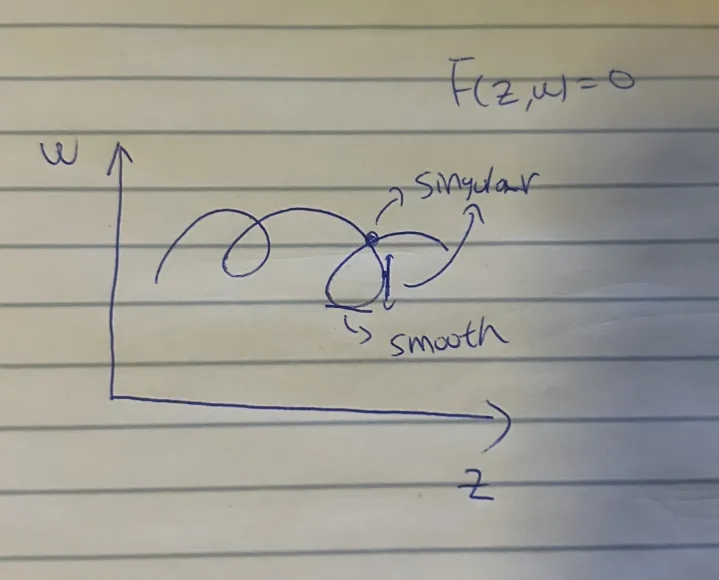
\includegraphics[width=0.5\textwidth]{Figures/lec6-1.png}.\]

Locally on $F(z, w) = 0$, we can parameterize $w = g(z)$ and consider $F(z, g(z)) = 0$. Then we hae that
\[0 = \frac{d}{dz} F(z, g(z)) = D_1 F + (D_2 F) g'(z).\]
Hence we can write
\[g'(z) = -\frac{D_1 F}{D_2 F}(z, g(z)).\]

\begin{question}
    Let $\alpha: [0, b] \to \Cbb$ be a branch of $g$ near $\alpha(0)$, when can we analytically continue along $\alpha$?
\end{question}

Note that if $D_2 F \neq 0$, we can apply the Inverse/Implicit Function Theorem for holomorphic functions to define $g(z)$ locally. If $D_2 F = 0$, then we can write $z = (w - w_0)^{n+1} + z_0$ for $F(z, w) = 0$ near $(z_0, w_0)$ for some power of $n$. \mattie{why talk about this?}\\

Hence, we can always analytically continue along $\alpha$ except when $D_2 F(z, g(z)) \to 0$ (ie. hitting a critical value) or $g(z) \to \infty$ for $z = \alpha(t)$ as $t \to t_0 \in [0, b)$ (ie. hitting an asymptotic value).

\begin{exercise}
    For a fixed $P(x, y) \in \Cbb[x, y]$, when can there be $\alpha: [0, 1] \to \Cbb^2$ such that
    \[P(\alpha(t)) \equiv 0, \]
    and $a^1(t) \to z_0 \in \Cbb$ and $a^2(t) \to \infty$ as $t \to 1$ ($a^1, a^2$ denotes the first and second coordinate of $\alpha$).
\end{exercise}

\begin{example}
    When $P(z, w) = zw - 1$, we could take $\alpha(t) = (1-t, \frac{1}{1-t})$.
\end{example}



\newpage
\section{Lecture Februrary 22nd}

\subsection{Meromorphic Functions}

Recall that for $U$ a domain in $\Cbb$, we say that $f$ on $U$ is a \textbf{meromorphic function} on $U$ if there exists $E \subseteq U$ that is discrete, such that $f: U \setminus \{E\} \to \Cbb$ is holomorphic, and $f$ has a pole at each point $e \in E$ (ie. the singularity should not be essential).\\

We can also think of $f$ as a holomorphic function $f: U \to \hat{\Cbb} = \Cbb \cup \{\infty\}$, and we take $E = f^{-1}(\{\infty\})$ to be discrete. 

\begin{definition}
    Let $X$ be a Riemann surface, we say a function $f$ on $X$ has \textbf{pole} (or removable singularity) at $e \in X$ if there exists $g: U \ni e \to \Cbb$ holomorphic such that the pointwise multiplication $fg: U \setminus \{e\} \to \Cbb$ has removable singularity at $e$.
\end{definition}

\begin{definition}
Let $X$ be a Riemann surface, a \textbf{meromorphic function} $f$ on $X$ if one of the following equivalent definition holds,
\begin{itemize}
    \item $f$ is meromorphic with respect to each charts.
    \item There exist discrete subset $E \subseteq X$ such that $f: X \setminus E \to \Cbb$ is holomorphic, and $f$ has pole at each $e \in E$.
    \item $f: X \to \hat{\Cbb}$ is holomorphic and $E = f^{-1}(\{\infty\})$ is a discrete subset of $X$ (in particular, we can't take the constant function to $\infty$). 
\end{itemize}
Intuitively, this means that ``$f$ is holomorphic except where it has poles". We will use $M(X)$ to denote the \textbf{space of meromorphic functions on $X$}.
\end{definition}

\begin{remark}
    Meromorphic functions are the same as function fields on compact Riemann surfaces. For example, $M(\hat{\Cbb}) = \Cbb(x)$.
\end{remark}

\begin{theorem}
    $M(X)$ is a field under pointwise multiplication.
\end{theorem}

\begin{proof}
    Exercise.
\end{proof}

Meromorphic functions satisfies a pullback construction as follows.\\

\begin{definition}
Let's suppose we have $X, Y$ are Riemann surfaces, and $f: Y \to X$ is proper, non-constant, and holomorphic (hence a branched cover of finite degree $d$). For any $g \in M(X)$, we can define the \textbf{pullback of $f$} as
\[f^*: M(X) \to M(Y),\quad f^*(g) = g \circ f,\]
and $f^*(g)$ is a meromorphic function on $Y$.    
\end{definition}

One can check that
\begin{proposition}
    $f^*: M(X) \to M(Y)$ is a field homomorphism and hence also injective. Note that this statement actually \underline{uses the fact that $X$ is connected}, this may not be a field homomorphism when $X$ is not connected (the meromorphic function would become direct sum of fields over each component).
\end{proposition}

This leads us to the following theorem
\begin{theorem}
    The degree $d$ holomorphic branched covers (or proper holomorphic non-constant maps) of any Riemann surface $X$ are in canonical one-to-one correspondence with degree $d$ extensions of $M(X)$. Specifically, given a degree $d$ branched cover $f: Y \to X$, we send it to $f^*: M(X) \to M(Y)$, and this will be a degree $d$ field extension and be a bijection (up to isomorphism classes).\\

    In more categorical languages, consider the following diagram
    % https://q.uiver.app/#q=WzAsNixbMCwwLCJZXzEiXSxbMiwwLCJZXzIiXSxbMSwxLCJYIl0sWzQsMSwiTShYKSJdLFszLDAsIk0oWV8xKSJdLFs1LDAsIk0oWV8yKSJdLFswLDIsImZfMSIsMl0sWzEsMiwiZl8yIl0sWzMsNCwiZl8xXioiXSxbMyw1LCJmXzJeKiIsMl0sWzAsMSwiXFxleGlzdCBnIl0sWzUsNCwiZ14qIiwyXV0=
\[\begin{tikzcd}
	{Y_1} && {Y_2} & {M(Y_1)} && {M(Y_2)} \\
	& X &&& {M(X)}
	\arrow["{f_1}"', from=1-1, to=2-2]
	\arrow["{f_2}", from=1-3, to=2-2]
	\arrow["{f_1^*}", from=2-5, to=1-4]
	\arrow["{f_2^*}"', from=2-5, to=1-6]
	\arrow["{\exist g}", from=1-1, to=1-3]
	\arrow["{g^*}"', from=1-6, to=1-4]
\end{tikzcd},\]
we say given $f_1, f_2$, there exists $g$ that makes both diagram commutes. (Exercise. complete a careful category theory statement of the theorem.)
\end{theorem}

\begin{proof}
    The proof will be broken into several steps,
    \begin{enumerate}
        \item Let $f: Y \to X$ be a degree $d$ branched cover, then we wish to show that
        \[[M(Y):  f^* M(X)] = d.\]
        For this we need the following results:
        \begin{itemize}
            \item (a) \textbf{Primitive element theorem:} If $F$ is a field of characteristic zero, $E$ is a finite extension of $F$, then there exists $y \in E$ such that $E = F(y)$. We will not prove this result.
            \item (b) If $Y$ is a Riemann surface, $y_1, ..., y_n \in Y$, $w_1, ..., w_n \in \Cbb$, then there exists $f$ a meromorphic function on $Y$ with $f(y_i) = w_i$ for all $i$. This is a deep theorem whose proof we will postpone to the next unit.
            \item (c) \textbf{Symmetric functions:} Let $e_k(x_1, ..., x_n) = \sum_{A \subseteq \{1, ..., n\}, |A| = k} \prod_{i \in A} x_i$ be the \textbf{$k$-th elementary symmetric polynomial}. For example we have that
            \[e_1(x_1, ..., x_n) = x_1 + ... + x_n, e_2(x_1, ..., x_n) = x_1 x_2 + x_1 x_3 + ... + x_1 x_n + x_2 x_3 + ..., \]
            \[e_n(x_1, ..., x_n) = x_1 ... x_n.\]
            The roots of the polynomial (in $x$)
            \[h(x) = x^n - \sum_{k=1}^n (-1)^k e_k(x_1, ..., x_n) x^{n-k}\]
            are $x_1, ..., x_n$ counting multiplicity.
            \item (d) There's a general fact that, if $h: X \to \hat{\Cbb}$ is continuous, and $h$ is meromorphic on $X \setminus E$ for $E$ a discrete subset of $X$, then $h$ is meromorphic function on $X$.
        \end{itemize}
        Now to prove (1), we first choose $q \in X$ such that $f$ is \textbf{not branched} over $q$. Now, we take $g \in M(Y)$ such that $g$ is finite on $f^{-1}(\{q\})$ and has $d$ distinct values (this uses result 1(b) that tells us we can specify the values of $g$ on a finite set).\\

        Near $q$, choose a neighborhood $U \ni q$ such that $f$ is a local homeomorphism on $U$ (recall that the branched values are discrete, so we can do this). Now, we can define $d$ branches of $f^{-1}$ here (call them $f_1^{-1}, ..., f_d^{-1}$) and we let $c_k(x) = e_k(g \circ f_1^{-1}, ..., g \circ f^{-1}_d)$. Note that $c_k(x) \in M(U)$.\\

        Now if $q$ is a branched value, its preimage (while not distinct) will have multiplicity $d$, so we can continuously extend $c_k(x)$ to $q$ by filling in the $d$ (with multiplicity) point in the preimage into the $d$ components of $c_k(x)$. Thus, we can do this for all $q \in X$ and define $c_k(x)$ locally. One can check that they agree on intersections.
        
        % we can similarly define the set theoretic function $c_k(x)$ on $q$ can actually be evaluated. This is because $f^{-1}(q)$ has some number $d'$ of points (which is not $d$), but in this case we consider the elementary symmetric function $c_k(g \circ f_1^{-1}, ..., g \circ f_{d'}^{-1})$.\\
        
        Hence, we have that these $c_k$'s are actually defined and meromorphic on $X \setminus \{\text{branched values of $f$}\}$. They also admit continuous extensions to the branched values and hence meromorphic on $X$.\\

        We can use 1(d) to guarantee that the \underline{$c_k$'s become a meromorphic function on $X$}. Then we have the equation using 1(c),
        \[g^d + \sum_{k = 1}^d (-1)^k f^*(c_k) g^{d-k} = 0 \text{ on $Y$}. \quad (\dagger)\]
        Hence the previous equation $(\dagger)$ above implies that the degree of field extension
        \[[f^*(M(X))(g): f^*(M(X))] \leq d.\]
        If $M(Y)$ is a finite field extension over $M(X)$, then by the Primitive Element Theorem (1(a)) we can choose appropriate $g$, we have that
        \[[M(Y): f^*(M(X))] \leq d.\]
        Now we observe that every element of $M(Y)$ has fintie degree over $M(X)$ by $(\dagger)$, so either $[M(Y): f^*(M(X))] < \infty$, or there exists $g_1, g_2, ...$ with $f^*(M(X))(g_1, ..., g_n)$ strictly increasing in and relatively finite. In the second case, we can choose $n$ large enough such that
        \[[f^*(M(X)(g_1, ..., g_n), f^*(M(X))] > d, \text{ which violates the primitive element theorem }.\]
        Thus, we have that $M(Y)/M(X)$ is a finite extension.\\

        Finally, let $P(X)$ be the minimal polynomial for $g$ (of degree $n$). We can write
        \[P(X) = x^n + \sum_{k=1}^n (-1)^k f^*(r_k) x^{n-k}, r_k \in M(X). \]
        then we have that 
        \[P(g) \equiv 0 \text{ on $Y$}.\]
        In particular, this means that 
        \[P(g)(q_i) = 0, \forall q_i \in f^{-1}(q), q \text{ is not branched value }. \quad (\Psi)\]
        Write $s_k = (-1)^k r_k(q) \in \Cbb$, if we look at
        \[p_q(x) = x^n + \sum_{k=1}^{n} s_k x^{n-k} \in \Cbb[x],\]
        this must have less than or equal to $n$ roots, but we also know that $p_q(g(q_i)) = 0$ from $(\Psi)$, and the values of $g(q_i)$ are distinct. Hence, $n \geq d$.\\

        Thus, the minimal polynomial $P(X)$ has degree at least $d$. By $(\dagger)$, it means that its degree is exactly $d$. Hence, we conclude that
        \[[M(Y): M(X)] = d.\]
        \item We did not get to proving the bijectivity part, it will hopefully be at the next lecture. As a sketch, given any field extension of degree $d$ over $M(X)$, we can write down the minimal polynomial generating the field extension, and the germs of solutions to its will be the branched cover.
\end{enumerate}
\end{proof}

\newpage
\section{Lecture February 27th}

\subsection{Constructing Branched Covers from Field Extensions}

Last time, we proved half of a theorem, which we will now try to prove the converse.
\begin{theorem}
    If $X$ is a Riemann Surface, and $E$ is a field extension of $M(X)$, with $[E: M(X)] = d < \infty$, then there exists a degree $d$ branched cover $f: Y \to X$, and $h: M(Y) \to E$ an isomorphism such that this diagram commutes
    % https://q.uiver.app/#q=WzAsMyxbMSwwLCJNKFgpIl0sWzIsMSwiRSJdLFswLDEsIk0oWSkiXSxbMCwxLCJcXHN1YnNldGVxIl0sWzAsMiwiZl4qIiwyXSxbMiwxLCJoLCBcXGNvbmciLDJdXQ==
\[\begin{tikzcd}
	& {M(X)} \\
	{M(Y)} && E
	\arrow["\subseteq", from=1-2, to=2-3]
	\arrow["{f^*}"', from=1-2, to=2-1]
	\arrow["{h, \cong}"', from=2-1, to=2-3]
\end{tikzcd}.\]
\end{theorem}

\begin{proof}
    By the Primitive Element Theorem, there exists a polynomial $P \in M(X)[T]$ of degree $d$ (in $T$) such that $E = M(X)(v)$ for $v \in E$ and $P(v) = 0$. Moreover, we can choose so that $P$ is the monic minimal polynomial of $v$.\\

    If the polynomial discriminant $\Delta P$ (which we can think of as the resultant of $P$ and $P' = \frac{\partial P}{\partial T}$) is not zero at $ q\in X$ and $P \neq \infty$ at $q \in X$, we can find an open set $U$ containing $q$ and $d$ solutions (meromorphic functions)
    \[g_1, ..., g_d: U \to \Cbb \text{ such that } P(g_i) \equiv 0 \text{ on $U$}.\]

    Here's an illustrative diagram demonstrating why we can find these solutions:
    \[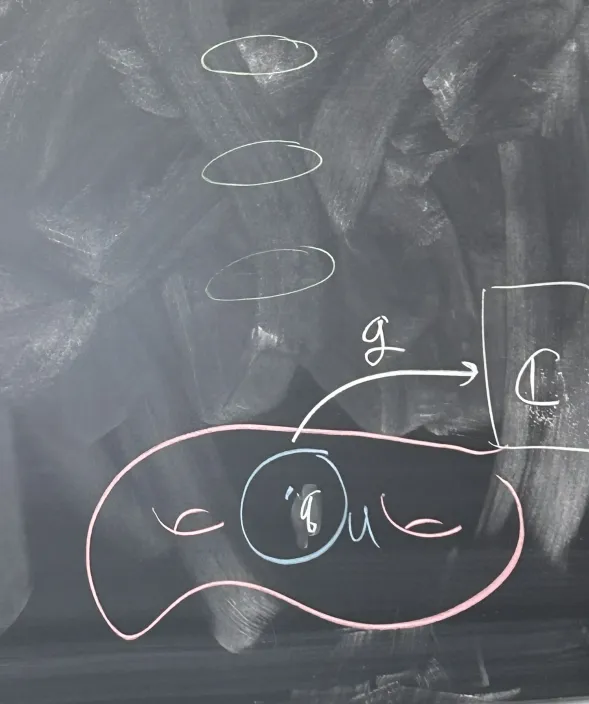
\includegraphics[width=0.5\textwidth]{Figures/lec8-1.png}\]
     We know that $P(T) = \sum_{k = 0}^{d} c_k(x) T^k$ where $c_k(x) \in M(X)$. Hence for $x = q$ is fixed, we can say that $P(q)[T] = \sum_{k = 0}^d c_k(q) T^k$ has coefficients in the complex numbers, ie. $P(q)[T] \in \Cbb[T]$ when $q$ is fixed. Because the discriminant is non-zero, there are $d$ distinct roots in the complex numbers, furthermore the roots move holomorphically with respect to $x$ and do not intersect in small enough $U$ (as long as $\Delta P$ is non-zero).\\

     Finding the functions $g_1, ..., g_d$ amounts to solving $P_2(q, g_i(q)) = 0$, where we define $P_2(q, w) = P(q)(w)$ (set $x = q$ and $T = w$).\\

     So the germs of $g$ such that $P(q, g(q)) = 0$ form a degree $d$ cover over $X \setminus \{z \in X\ |\ P(z)[T] \notin \Cbb[T] \text{ or } \Delta P(z) = 0\}$. We call the set being subtracted $E$.\\

     Note that clearly $E$ is discrete, so we can complete this cover to a degree $d$ branched cover $Y$ of $X$ over $E$. Note that $E$ will not be discrete if $\Delta P$ is identically zero, this is because we are working over a characteristic zero field and irreducible implies separable. Furthermore, now $g$ is a meromorphic function on $Y$ with $P(g) = 0$.
\end{proof}

\begin{question}
    An automorphism of the Riemann surface $X$ induces an automorphism on the field of Meromorphic functions on $X$. Is this process surjective? In other words, does a field automorphism on $M(X)$ come from an automorphism of $X$.
\end{question}

\subsection{The Mittag-Leffler Problem}

The second unit is about classical theorems on (mostly) compact Riemann surfaces (e.g. $X$).\\

To motivate the first discussion of the unit, we will begin with the \textbf{Mittag-Leffler Problem}.

\begin{question}[Mittag-Leffler Problem]
    Let $X$ be a compact Riemann surface, find $f \in M(X)$ with specified ``principal parts".\\
    
    Suppose $\{q_i\}$ is a collection of discrete points on $f \in M(X)$, we can write each $q_i$ with a coordinate chart $q_i \in V_i$ and $\varphi_i: U_i \to \hat{\Cbb}$. Let's suppose without loss that $\varphi_i(q_i) = 0$, then we can write the power series expansion
    \[f|_{U_i} \circ \varphi_i^{-1}(z) = \sum_{k = -m}^\infty c_k z^k \text{ on $V$}.\]
    With some abuse of notation, when the context is clearly, we will just write $f \circ \varphi_i^{-1}$ as ``$f$ in the coordinate $\varphi_i$".
    \[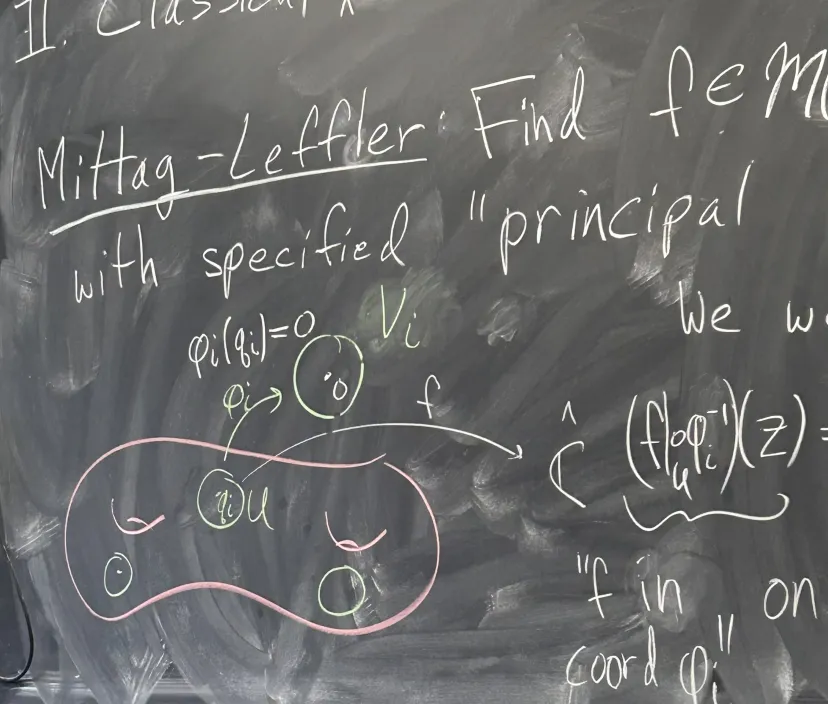
\includegraphics[width=0.5\textwidth]{Figures/lec8-2.png}\]
    In this case, our goal is given $c_{-1}, ..., c_{-m}$ for each $i$, we can construct a meromorphic function $f \in M(X)$ whose $c_{-1}, ..., c_{-m}$ is the specified given values.
\end{question}

Equivalently, this problem may be stated as follows.
\begin{question}
    Given finite set $(U_i, q_i, h_i \in M(U_i)$ such that $h_i|_{U_i - \{q_i\}}$ is holomorphic (it can only have pole on $q_i$). Find $f \in M(X)$ such that $f$ is holomorphic on $X - \{q_i\}_i$ and $f|_{U_i} - h_i$ is holomorphic on $U_i$.
\end{question}

The following proposition shows that the first question can be rephrased in a coordinate-independent way.
\begin{proposition}
    If $f_1, f_2: U_i \to \hat{\Cbb}$ are holomorphic on $U_i \setminus \{q_i\}$, then $f_1 - f_2$ is holomorphic on $U_i$ if and only if $f_1$ and $f_2$ have the same principal part at $q_i$.
\end{proposition}

To solve the Mittag-Leffler Problem, we wish to find $g: X \to \hat{\Cbb}$ such that
\begin{itemize}
    \item $g \equiv h_i$ on some $U_i'$ compactly contained in $U_i$ and $q_i \in U_i'$,.
    \item $g$ is smooth and finite on $X \setminus \{q_i\}$.
    \item In this case, $g$ is a ``weak solution" to the Mittag-Leffler problem.
    \item We want to correct $g$ to a meromorphic function. We do this by adding some function $h$ (with $h$ holomorphic on $U_i'$) to $g$ such that $g + h \in M(X)$.
\end{itemize}

\begin{question}
    How do we find such $h$?
\end{question}

To find $h$, we want it to be a solution to the equation
\[\overline{\partial} h = - \overline{\partial} g\]
on $X$, where $\overline{\partial}$ is to be defined. Then, $\overline{\partial} h  = 0$ on each $U_i' \setminus \{q_i\}$ and $\overline{\partial}(g + h) \equiv 0$ on $X \setminus \{q_i\}$.\\

We want $\overline{\partial}$ to be a differential operator such that 
\[\overline{\partial} f \equiv 0 \text{ on $U$ } \iff f \text{ is holomorphic on } U.\]

\subsection{$\overline{\partial} f$ on the Complex Plane}

Let $U$ be a connected open set in $\Cbb$, and $f \in C^\infty(U)$. We seek to define $\overline{\partial} f \in C^\infty(U)$. Here are some properties, the operator should respect,
\begin{enumerate}
    \item $\overline{\partial}(f(z) + a) = \overline{\partial}(f(z))$, for $a \in \Cbb$.
    \item  $\overline{\partial}(z \mapsto f(z+a)) = z \mapsto \overline{\partial}(f(z + a))$.
    \item  $\overline{\partial}(cf(z)) = c\overline{\partial}(f(z))$.
    \item  $\overline{\partial}(f(z) + g(z)) = \overline{\partial}(f(z)) + \overline{\partial}(g(z))$.
    \item $\overline{\partial}(z \mapsto z) = 0$.
    \item $\overline{\partial}(z \mapsto \overline{z}) = 1$.
    \item $\overline{\partial}(f(z)) = 0$ if $Df(z) = 0$ (all of its first derivatives are zero).
\end{enumerate}

As a consequence of these axioms, we should have that
\[\overline{\partial}(Az + B \overline{z}) = B.\]
We can write any smooth function as
\[f(z) = f(z_0) + A (z - z_0) + B(\overline{z - z_0}) + O(|z - z_0|^2).\]

Using the summation above, if we compute the real partial derivatives, we will get that 
\[\frac{\partial f}{\partial x}(z_0) = A + B.\]
\[\frac{\partial f}{\partial y}(z_0) = i (A - B).\]

We can solve these equations to get
\[A = \frac{1}{2}(\frac{\partial f}{\partial x} - i \frac{\partial f}{\partial y}), B = \frac{1}{2} (\frac{\partial f}{\partial x} + i \frac{\partial f}{\partial y}).\]
In this case, we write that
\[\frac{\partial f}{\partial z} = A \text{ and } \frac{\partial f}{\partial \overline{z}} = B.\]
Sometimes we also write them as $\partial_z f$ and $\partial_{\overline{z}} f$.

Now in this case, $f$ has a complex derivative at $z_0$ if and only if $\frac{\partial f}{\partial \overline{z}}(z_0) = 0$. 

\newpage
\section{Lecture February 29th}

\textbf{Recall:} Last time, we introduced the Mittag-Leffler problem.
\begin{enumerate}
    \item We want to make meromorphic functions on $X$ with specified principal parts.
    \item We can make them by finding ``weak solutions" (meromorphic near specifications and $C^\infty$ else where). Then we can correct the weak solutions by solving the equation $\overline{\partial} h = \alpha$, where $\alpha = \overline{\partial} g$ and $g$ is the weak solution.
    \item For two variable smooth functions on the complex plane, if $f(z) = f(z_0) + A(z - z_0) + B(\overline{z - z_0}) + \mathcal{O}(|z - z_0|^2)$, then we define $\partial_z f \coloneqq A$ and $\partial_z f \coloneqq B$. Then we can derive that
    \[\partial_x f = A + B \text{ and } \partial_y f = i(A - B).\]
    In this case, sooving for $A$ and $B$ gives us that
    \[\partial_z f = A = \frac{1}{2} (\partial_x f - i \partial_y f) \text{ and } \overline{\partial}_z f = B = \frac{1}{2}(\partial_x f + i \partial_y f)\]
\end{enumerate}

\begin{remark}
    In the language of differential forms, we can write
    \[dz \coloneqq dx + idy \text{ and } \overline{dz} = dx - idy.\]
    In this case we have that
    \[d\overline{z} \wedge dz = i dx \wedge dy - i dy \wedge dx = 2i (dx \wedge dy).\]
    Furthermore, this means that as exterior derivatives we can write
    \[df = \partial_x f dx + \partial_y f dy = \partial_z f dz + \partial_{\overline{z}} f \overline{dz}.\]
\end{remark}

\begin{theorem}
    If $U \subseteq \Cbb$ is compact with piecewise $C^1$ boundary $\partial U$, and $f: U \to \Cbb$ is $C^1$, 
    \[\int_{\partial U} f(z) dz = 2i \int_{U} \partial_{\overline{z}} f(z) dx dy, z = x + iy.\]
    Note that the RHS is equal to $\int \partial_{\overline{z}} f(z) d\overline{z} \wedge dz = \int_U df \wedge dz$ (in the language of Differential Forms). In other words, this is simply an application of Stoke's Theorem for differential forms.
\end{theorem}

\begin{proof}
    We will present an elementary proof without using the generalized Stoke's Theorem. We first prove this when $U$ is a rectangle with sides $A, B, C, D$ oriented as
    \[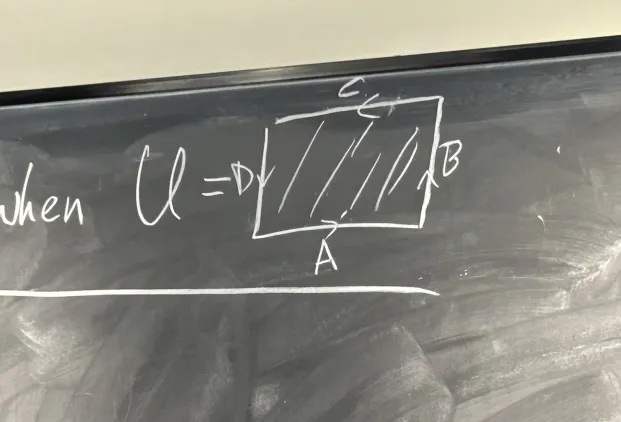
\includegraphics[width=0.5\textwidth]{Figures/lec9-1.png}\]
    Indeed, we can compute the integral to see that
    \begin{align*}
        \int_{U} \partial_{\overline{z}} f dx dy &= \frac{1}{2} \int_{U} \partial_x f dx dy + \frac{i}{2} \int_{U} \partial_y f dx dy\\
        &= \frac{1}{2} \left(\int_B f dy - \int_D f dy \right) + \frac{i}{2} \left( \int_C f dx - \int_A f dx \right) \tag*{Fundamental Theorem of Calculus with respect to one variable}\\
        &= \frac{1}{2} (\int_{B} f \frac{dz}{i} - \int_{D} f \frac{-dz}{i}) + \frac{i}{2} (\int_{C} f(-dz) - \int_{A} f dz) \tag*{Recall $dz = dx + idy$}\\
        &= \frac{1}{2i} \int_{\partial U} f dz.
    \end{align*}
    More a general $U$, we can approximate it by an open set with polygonal boundary, which itself can be approximated by an open set with boundaries composed of vertical and horizontal line segments (which can then be broken down into rectangles).
\end{proof}

\begin{exercise}
        Make the discussion for the general case rigorous.
    \end{exercise}

Recall that for $f: X \to \Cbb$ (or replace $\Cbb$ with any vector space), then
\[\operatorname{supp} f = \operatorname{closure}(\{x \in X\ |\ f(x) \neq 0\}).\]

\begin{definition}
Now suppose $f: \Cbb \to \Cbb$ has compact support, meaning that $\operatorname{supp}(f) \subseteq D_R$ for some $R > 0$. For any $z \in \Cbb$, we define
\[Pf(z) \coloneqq \frac{1}{\pi} \int_{\Cbb} \frac{f(\zeta)}{z - \zeta} d\xi d\eta,\quad \zeta = \xi + i \eta.\]
Is this well-defined? Is this absolutely convergent or are we talking about a principal value? Well, rewriting this in polar coordinates, we write $\zeta = z + r e^{i\theta}$, we have that the integral is
\[Pf(z) \coloneqq \frac{1}{\pi} \int_{0}^{\infty} \int_{0}^{2\pi}  \frac{f(z + re^{i\theta})}{-r e^{i\theta}} r d\theta dr\]
\[= \frac{-1}{\pi} \int_0^\infty \int_0^{2\pi} f(z + r e^{i \theta}) e^{i \theta} dr d\theta.\]
\[= \frac{-1}{\pi} \int_0^{R + |z|} \int_0^{2\pi} f(z + r e^{i \theta}) e^{i \theta} dr d\theta, \quad \text{$f$ has compact support}\]
which implies that the integral is absolutely convergent.
\end{definition}

Hence, $Pf(z)$ is convergent and well-defined. Furthermore, our estimate gives us a proof that
\begin{proposition}
    $|Pf(z)| \leq 2 (R + |z|) ||f||_\infty$. 
\end{proposition}

Similarly, because of the absolute convergence, we will also have that
\begin{proposition}
    Suppose $f$ is $C^{|\alpha|}$, then
    $$D_\alpha Pf(z) = P(D_\alpha f)(z)$$,
    where $D_\alpha = \frac{\partial}{\partial x^k} \frac{\partial}{\partial y^\ell}$ and $|\alpha| \coloneqq k + \ell$.
\end{proposition}

This leads us to the following theorem.
\begin{theorem}
    For $f: \Cbb \to \Cbb$ that is a $C^1$ function with compact support, then
    \[(\partial_{\overline{z}} Pf)(z) = f(z).\]
    Note that this means that $Pf$ is holomorphic outside of the support of $f(z)$.
\end{theorem}

\begin{proof}
    It suffices for us to show that for all rectangles $U$, 
    \[\int_{U} \partial_{\overline{z}} Pf(z) dx dy = \int_{U} f(z) dx dy.\]
    By our version of Green's Theorem derived earlier in this lecture, we have that
    \begin{align*}
        \int_U \partial_{\overline{z}} Pf(z) dx dy &= \frac{1}{2i} \int_{\partial U} Pf(z) dz\\
        &= \frac{1}{2i} \int_{\partial U} \left(\frac{1}{\pi}\int_{D_{R + |z| + 1}} \frac{f(\zeta)}{z - \zeta} d\xi d\eta \right) dz\\
        &= \frac{1}{2i} \int_{D_{R + |z| + 1}} f(\zeta) \left(\frac{1}{\pi}\int_{\partial U} \frac{dz}{z - \zeta}\right) d\xi d\eta \tag*{Fubini-Tonelli Theorem because of absolute convergence}
    \end{align*}
    What is the integral $\int_{\partial U} \frac{dz}{z - \zeta}$? Well it is the winding number of $\partial U$ around $\zeta$ multiplied with $2 \pi i$. Hence we have that
    \[\int_{\partial U} \frac{dz}{z - \zeta} = 2\pi i \mathbbm{1}_{U}(\zeta) = 2\pi i \chi_U(\zeta).\]
    Hence we have that
        \begin{align*}
        \int_U \partial_{\overline{z}} Pf(z) dx dy &= \frac{2\pi i}{2\pi i} \int_{D_{R + |z| + 1}} f(\zeta) \chi_U(\zeta) d\xi d\eta\\
        &= \int_{U} f(\zeta) d\xi d\eta.
    \end{align*}
\end{proof}

\begin{theorem}
    The following are equivalent for $\operatorname{supp}(f) \subseteq D_R$ and $f \in C^1$,
    \begin{enumerate}
        \item $\operatorname{supp}(Pf)$ is compact.
        \item $\operatorname{supp}(Pf) \subseteq D_R$.
        \item $\int_{D_R} fh = 0$ for all holomorphic functions $h: D_R \to \Cbb$.
    \end{enumerate}
\end{theorem}

\begin{proof}
   Clearly (2) implies (1). Now for (1) implies (2), we know that $Pf$ is holomorphic outside of the support of $f$ from the last theorem, hence $Pf$ is holomorphic outside of $D_R$. On the other hand, we know that $Pf \equiv 0$ near $\infty$ because we assumked $\operatorname{supp}(Pf)$ is compact, hence $Pf \equiv 0$ outside of $D_R$ by the identity theorem.\\

   For (3) implies (2), in this case, we have that $Pf(z) = \int_{D_R} \frac{f(\zeta)}{\zeta - z} d\xi d\eta$. We can write the RHS as
   \[Pf(z) = \int_{D_R} f h_z, h_z(\zeta) = \frac{1}{\zeta - z},\]
   and $h_z(\zeta)$ will be a holomorphic function as long as $z \notin D_R$. Hence, by (3), we have that
   \[Pf(z) = 0, \forall z \notin D_R.\]

   For (2) implies (3), we can write
   \[\int_{D_R} fh = \int_{D_{R'}} f h, \text{ for some } R' < R\]
   This is just a technical point to get $h$ continuous on boundary. In this case we have that
   \begin{align*}
       \int_{D_{R'}} fh &= \int_{D_{R'}} (\partial_{\overline{z}} Pf) h\\
       &=  \int_{D_{R'}} \partial_{\overline{z}}( (Pf)h)\tag*{$\partial_{\overline{z}}(gh) = \partial_{\overline{z}}(g) h + g (\partial_{\overline{z}}(h)) = \partial_{\overline{z}}(g) h + 0 $}\\
       &= \int_{\partial D_{R'}} Pf(z) h(z) dz\\
       &= 0 \tag*{Support of $Pf(z)$ is contained in $D_R$.}
   \end{align*}
\end{proof}

\newpage
\section{Lecture March 5th}
Let $U \subseteq \Cbb$ be an open connected set. Let $\mathcal{E}(U) \coloneqq C^\infty(U)$. For any $f \in \mathcal{E}(U)$, we have that
\[D_\alpha f \coloneqq \frac{\partial^{k+\ell}}{\partial x^k \partial y^\ell} f \in \mathcal{E}(U),\]
where $\alpha = (k, \ell) \in \Nbb^2$ is a multi-index and $|\alpha| = k + \ell$.\\

For $m \in \Nbb$ and $K \subseteq U$ compact, we define
\[||f||_{m, K} \coloneqq \sup_{z \in K, |\alpha| \leq m} |D_\alpha f(z)|.\]

We can take a compact exhaustion $K_n$ of $U$ with $K_n \subseteq \operatorname{Int}(K_{n+1})$ and $\bigcup K_n = U$. We can define
\[||f||_{m, n} \coloneqq ||f||_{m, K_n}.\]

We define a topology on $\mathcal{E}(U)$ with the condition that $\lim_{t \to \infty} f_t \to f$ if and only if for all $m, n$, 
\[\lim_{t \to \infty} ||f_t - f||_{m, n} \to 0.\]

\subsection{Topological Vector Space}

\begin{definition}
    A \textbf{topological vector space} $V$ is a vector space over $\Rbb$ or $\Cbb$ (denote the field as $\mathbb{F}$) with a Hausdorff topology $\tau$ on $V$ such that the following maps are continuous:
    \begin{enumerate}
        \item $V \times V \to V$ given by $(x, y) \mapsto x + y$.
        \item $\mathbb{F} \times V \to V$ given by $(\lambda, x) \mapsto \lambda x$.
    \end{enumerate}
\end{definition}

\begin{definition}
    A \textbf{seminorm} on a vector space $V$ is a map $||\bullet||: V \to [0, \infty)$ such that
    \begin{enumerate}
        \item $||f + g|| \leq ||f|| + ||g||$.
        \item $||\lambda f|| = |\lambda| ||f||$.
    \end{enumerate}
    A seminorm is furthermore a norm if additionally $||f|| = 0$ implies that $f = 0$.
\end{definition}

\begin{definition}
Given a collection of seminorms $\{||\bullet||_\alpha\ |\ \alpha \in A\}$ such that if for all $\alpha$, $||f||_\alpha = 0$, then $f = 0$.\\

We can define a \underline{topology} on $V$ generated by the open sets of the form
\[\{B_{\alpha, r}(g) \coloneqq \{f\ |\ ||f - g||_\alpha < r\}, \]
indexed over all $\alpha$ and all $r$.
In this case, $V$ is called a \textbf{locally convex topological vector space}.
\end{definition}

\begin{definition}
    A \textbf{Frechet} space is a locally convex topological vector space from a family of seminorms indexed by $\alpha$. The topology is metrizable, and we can convert this into a metric by
    \[d(f, g) \coloneqq \sum_{\alpha = 1}^\infty 2^{-\alpha} h(||f - g||_\alpha),\]
    where $h(x) = \frac{x}{1 + x}$. We also want to require that this metric is complete.
\end{definition}

\begin{example}
    For $f \in C^0(U)$ (the continuous functions), and $K_n$ is a compact exhaustion of $U$, we can define 
    \[||f||_n \coloneqq \sup_{x \in K_n} |f(x)|.\]
    This is indeed a family of seminorms (they are not norms!) Hence we can give a topology on $C^0(U)$ as a Frechet space. This is also the \textbf{topology of uniform convergence on compact sets (normal convergence)}.
\end{example}

Let $D(U) \coloneqq = \{f \in \mathcal{E}(U)\ |\ \operatorname{supp}(f) \text{ is compact}\}$ (ie. $C^\infty_0(U)$). We also \underline{want a topology} on $D(U)$ such that $f_n \to f$ in $D(U)$ if and only if $f_n \to f$ in $\mathcal{E}(U)$ AND there exists compact $K \subseteq U$ such that for all $n$,
\[\operatorname{supp} f_n \subseteq K.\]

\begin{remark}
   The topology we seek on $D(U)$ is certainly not the subspace topology. 
\end{remark}

\begin{definition}
    The topology we will construct is as follows. For any $h; U \to [0, \infty)$ continuous and $m \in \Nbb$, for any $f \in D(u)$, we let 
    \[||f||_{h, m} \coloneqq \sup_{z \in U, |\alpha| \leq m} h(z) |D_\alpha f(z)|.\]
    These semi-norms define the topology of $D(U)$ as described in the definition earlier. (This is not a Frechet space because the family is not countable).
\end{definition}

\begin{exercise}
    Show that this definition agrees with the topology we wanted to construct.
\end{exercise}

We will also leave the folllowing theorem as an exercise.
\begin{theorem}
    Let $U, V$ be domains in $\Cbb$. If $g: U \to V$ is a diffeomorphism, then $g^*: \mathcal{E}(V) \to \mathcal{E}(U)$ (resp. $g^*: D(V) \to D(U)$) given by
    \[g^* f = f \circ g\]
    is an isomorphism of topological vector spaces.
\end{theorem}

\subsection{Distribution}

\begin{definition}
    A \textbf{distribution} $T \in D(U)^*$ on $U$ is $\Cbb$-valued continuous $\Cbb$-linear functional on $\mathcal{D}(U)$.
\end{definition}

\begin{example}
    If $g \in C^0(U)$, then we can define
    \[\underline{g}: D(U) \to \Cbb\]
    defined by
    \[\underline{g}(f) = \int_{U} fg.\]
    Note that this is well-defined because $f$ is compact support, and this is a distribution.
\end{example}

More generally, if $\mu$ is any locally finite signed Borel measure on $U$ (locally finite means on any compact set it should have finite measure), then the map
\[f \mapsto \int_{U} f d\mu\]
is a distribution.\\

Even more generally, suppose $(\mu_\alpha)_{|\alpha| \leq m}$ is a collection of these kind of measures, then
\[f \mapsto \sum_{\alpha} \int D_\alpha f (d\mu_\alpha) \in D(U)^*.\]

\subsection{Weyl's Lemma}

\begin{theorem}[Holomorphic Weyl's Lemma]
   Let $U \subseteq \Cbb$ be a domain. If $F \in D(U)^*$ is a distribution such that
   \[F(\overline{\partial}g) = 0, \forall g \in D(U),\]
   then there exists $f $ holomorphic on $U$ such that
   \[F = \underline{f}.\]
   In other words, we have that
   \[F(g) = \int_{U} fg, \forall g \in D(u).\]
\end{theorem}

\begin{remark}
    There's also a version of the theorem where $\overline{\partial} g$ is replaced woth $\Delta g$. This is the harmonic version of Weyl's Lemma usually seen in PDEs.
\end{remark}

To prove Weyl's Lemma, we want to make sense of differentiation of distributions (otherwise known as a weak derivative). 
\begin{definition}[Weak Derivative]
    For multindex $\alpha \in \Nbb^2$ and $f \in \mathcal{E}(U)$ and $g \in D(U)$, then
    \begin{align*}
        \int_{U} (D_\alpha f) g \coloneqq (-1)^\alpha \int_{U} f D_\alpha g \tag*{Repeated Integration By Parts}.
    \end{align*}
    This motivates a definition where we define for $T \in D(u)^*$ a distribution as
    \[(D_\alpha T)(g) \coloneqq (-1)^{|\alpha|} T(D_\alpha g).  \]
\end{definition}

\begin{example}
    Let $T \in D^*(U)$ be a distribution. We define $\partial_{\overline{z}} T$ as
    \[\partial_{\overline{z}} T \coloneqq \frac{1}{2} (\partial_x T + i \partial_y T),\]
    where $\partial_x T$ and $\partial_y T$ are defined in the weak sense.\\

    Note that this means that $T(\overline{\partial} g) = \partial_{\overline{z}} T$.
\end{example}


\begin{theorem}
    Suppose $U, V \subseteq \Cbb$ are domains, $g \in D(U \times V)$ (with coordinates $\zeta$ and $z$), and $T \in D(U)^*$, then
    \[D_\alpha(z \mapsto T(\zeta \mapsto g(\zeta, z))\ ) = T(\zeta \mapsto D_\alpha (z \mapsto g(\zeta, z)\ ). \]
\end{theorem}

\begin{proof}
    Exercise.
\end{proof}

\begin{theorem}
    Suppose $U, V \subseteq \Cbb$ are domains, $g \in D(U \times V)$ (with coordinates $\zeta$ and $z$), and $T \in D(U)^*$, then
    \[\int_{U} T(\zeta \mapsto g(\zeta, z)) dx dy = T(\zeta \mapsto \int_{U} g(\zeta, z) dx dy).\]
\end{theorem}

\begin{proof}
    Exercise.
\end{proof}

\newpage
\section{Lecture March 7th}

\subsection{Convolution on Distributions}

Given functions $f, g$, the idea of a convolution is that we want to define the colvution of $f$ and $g$,
\[(f \star g)(z) \coloneqq \int f(\zeta) g(z - \zeta) d\xi d\eta.\]
Of course, the question is where are they define?

Indeed, we want $z \in U$ (where $U$ is a domain), $f \in \mathcal{E}(n_r(U))$, and $g \in D(\mathbb{D}_r)$. Here, $n_r(U)$ refers to a neighborhood of $U$ with ``radius $r$, that is
\[n_r(U) \coloneqq \bigcup_{z \in U} B_r(z).\]
For the sake of notation, we also define the ``$-r$ neighborhood of $U$" as
\[n_{-r}(U) \coloneqq \{z \in U\ |\ B_r(z) \subseteq U\}.\]

Note that we have the relation that
\[n_{-r}(U) \subseteq U \subseteq n_{r}(U).\]

\begin{definition}
    In the set up above, we define
\[(f \star g)(z) = \int_{n_r(U)} f(\zeta) g(z - \zeta) d\xi d\eta.\]
\end{definition}

Here are some standard properties of convolution that one should try as exercises.
\begin{proposition}
    In the set up above, we have that
    \[f \star g = g \star f \text{ and } f \star (g \star h) = (f \star g) \star h.\]
\end{proposition}

We could extend the notion of convolution to distributions.
\begin{definition}\label{def:conv_dist}
 Suppose $T \in D(n_r(U))^*$ is a distribution and $g \in D(\mathbb{D}_r)$, we define 
 \[(T \star g)(z) \coloneqq T(\zeta \mapsto g(z - \zeta)).\]
 Furthermore, $T \star g \in \mathcal{E}(U)$ (ie. it's a smooth function on $U$). Finally, for all $h \in D(U)$,
 \[\int (T \star g) h = T(g \star h). \]
 Note that these two properties essentially follows from the fact that distributions commute with differentiation and integrations (Exercise).
\end{definition}

Take $\psi \in D(\mathbb{D}_1)$ such that 
\[\int \psi = 1, \psi(\mathbb{D}_1) \subseteq [0, \infty), \psi(\rho z) = \psi(z) \text{ for all } \rho \in S^1 \subseteq \Cbb.\]
In other words, $\psi$ is a rotationally symmetric bump function. Now we define that
\[\psi_{r}(z) = \frac{1}{r^2} \psi(\frac{z}{r}).\]
Note that $\psi_r \in D(\mathbb{D}_r)$ (is compactly supported in $\mathbb{D}_r$) and $\int \psi_r = 1$.\\

For $h: \mathbb{D}_r \to \Cbb$ holomorphic, we have that
\begin{align*}
    \int_{\mathbb{D}_r} h(z) \psi_r(z) dx dy &= \int_0^r \int_0^{2\pi} h(re^{i\theta}) \psi(r) r d\theta dr \tag*{$\psi$ is rotationally symmetric}\\
    &= \int_0^r 2\pi h(0) \psi(r) r dr d\theta \tag*{Mean Value Property} \\
    &= h(0) \int_{0}^r \int_{0}^{2\pi} \psi(r e^{i \theta}) r dr d\theta\\
    &= h(0) \int \psi\\
    &= h(0) (1)\\
    &= h(0).
\end{align*}

Hence, this property implies that for $r' < r$, for all holomorphic functions $h \in D(\mathbb{D}_r)$,
\[\int_{\mathbbm{D}_r} (\psi_r - \psi_{r'}) h = 0.\]
Hence, from last Thursday's last theorem, since $(\psi_r - \psi_{r'})$ annihilates all holomorphic functions, we have that $\psi_r - \psi_{r'} = \overline{\partial} q$ for some $q \in D(\mathbb{D}_r)$.\\

The paragraph above implies the following fact - Let $F \in D(U)^*$ is a distribution. If $F(\overline{\partial} q) = 0$ for all $q \in D(U)$, then
\[F \star (\psi_r - \psi_{r'}) = 0 \text{ on $D(n_{-r}(U))$}. \]
(Here, $\mathbb{D}_r$ happens to be a disk of radius $r$ contained in $U$).\\

Here's an illustrative picture of what is happening
\[\]

\subsection{Proof of Weyl's Lemma}

Recall that Weyl's Lemma is stated as follows.
\begin{theorem}
    Suppose $F \in D(U)^*$ is a distribution such that $F(\overline{\partial} q) = 0$ for all $q \in D(U)$, then there exists $f $ holomorphic on $U$ such that
   \[F = \underline{f}.\]
\end{theorem}

\begin{proof}
    We let $f_r = F \star \psi_r \in \mathcal{E}(n_{-r}(U))$. Then because we proved earlier that $F \star (\psi_r - \psi_{r'}) = 0$, we have that $f_r \equiv f_{r'}$ on $n_{-r}(U)$ for all $r' < r$.\\

    Now, we define our official $f$ for Weyl's Lemma as
    \[f \equiv f_r \text{ on } n_{-r}(U), \forall r \in \Rbb_{> 0}.\]
    Now we claim that $F = \underline{f}$. Equivalently, this means that we want to show - for all $g \in D(U)$, $F(g) = \int fg$. Indeed, for $r$ small,
    \begin{align*}
        \int fg &= \int f_r g \tag*{$g$ is supported in $n_{-r}(U)$ for sufficiently small $r$.}\\
        &= \int (F \star \psi_r) g\\
        &= F(\psi_r \star g) \tag*{Appeared in Definition~\ref{def:conv_dist}}
    \end{align*}
    Furthermore, we have that $\psi_r \star g \to g$ in $D(U)$ (with respect to the topology on $D(U)$) as $r \to 0$. Hence $F(\psi_r \star g) \to F(g)$ as $r \to 0$.\\

    Finally, we need to show that $f$ is holomorphic. Indeed, 
    \[\underline{\overline{\partial} f} = \overline{\partial} \underline{f} = \overline{\partial} F = 0.\]
    The first equality follows from commuting integral with the operator. Note that $\overline{\partial} F = 0$ because by integration by parts, for all $g \in D(U)$
    \[- \int_{U} (\overline{\partial f} g) = \int_{U} f \overline{\partial} g = F(\overline{\partial} g) = 0,\]
    and hence $\overline{\partial} F = 0$.
\end{proof}

\begin{exercise}
    Show that if $\Delta F = 0$ for $F \in D(U)^*$ , then $F = \underline{f}$ for some $f$.
\end{exercise}

\begin{exercise}
    Do Exercise $1$ in $\Rbb^n$.
\end{exercise}

\subsection{Complex Differential Forms}

Now we will carry the discussion back to a general Riemann surface. Let $X$ be a Riemann surface, we define the notations:
\begin{enumerate}
    \item $\mathcal{E}(X) = \{g: X \to \Cbb \text{ that are } C^\infty\}$.
    \item $\mathcal{E}^{(1)}(X) = \{$complex-valued smooth $1$-forms on $X\}$.
    \item $\mathcal{E}^{(2)}(X) = \{$complex-valued smooth $2$-forms on $X\}$.
\end{enumerate}

But what does ``complex-valued forms" mean?
\begin{definition}
    If $\alpha \in \mathcal{E}^{(1)}(X)$, then for all $z \in X$,
    \[\alpha(z): T_z(X) \to \Cbb \text{ is $\Rbb$-linear},\]
    where $T_z(X)$ is the tangent space at $z$. Given a chart $\varphi: U \subseteq X \to \Cbb$, we can consider $a_\varphi$ on $\varphi(U)$ as the pullback
    \[a_\varphi \coloneqq (\varphi^{-1})^*(\alpha) = \alpha^x_{\varphi} dx + \alpha^y_{\varphi} dy, \]
    where $dx((v^0, v^1)) = v^0$ and $dy((v^0, v^1)) = v^1$.\\

    We also define $\mathcal{E}^{1, 0}, \mathcal{E}^{0, 1} \subseteq \mathcal{E}^{(1)}$ such that
    \[\mathcal{E}^{1, 0} = \{\alpha \in \mathcal{E}^{(1)}\ |\ \alpha_z \text{ is } \Cbb-\text{linear for all $z \in X$}\}.\]
     \[\mathcal{E}^{0,1} = \{\alpha \in \mathcal{E}^{(1)}\ |\ \alpha_z \text{ is } \Cbb-\text{anti-linear for all $z \in X$}\}.\]
     (by anti-linear we mean $\alpha_z(\lambda v) = \overline{\lambda} \alpha_z(v)$.) Furthermore, we have that
     \[\mathcal{E}^{(1)} = \mathcal{E}^{1, 0} \oplus \mathcal{E}^{0, 1}.\]
     \[(\operatorname{Lin}_\Rbb(T_z(X), \Cbb)) = (\operatorname{Lin}_\Cbb(T_z(X), \Cbb) \oplus (\operatorname{AntiLin}_\Cbb(T_z(X), \Cbb)).\]

     The observant reader might notice that $\lambda v$ is actually done in $T_z(X)$ which is a tangent space. The idea is to do the multiplication by $\Cbb$ on a coordinate chart, which turns out to be well-defined.\\
\end{definition}

\begin{example}
    If $U \subseteq \Cbb$ is an open set, then we can think of $dz, d\overline{z} \in \mathcal{E}^{(1)}(\Cbb)$ in the context of the definition above,
\[dz(z)(v) = v \text{ and } \overline{dz}(z)(v) = \overline{v}. \]
In this case, we can think of
\[\mathcal{E}^{1, 0}(U) = \{\alpha dz \ |\ \alpha \in \mathcal{E}(U)\}\]
\[\mathcal{E}^{0, 1}(U) = \{\alpha \overline{dz}\ |\ \alpha \in \mathcal{E}(U)\}.\]
Hence the entire space of $\mathcal{E}^{(1)}(U)$ is of the form
\[\alpha dz + \beta \overline{dz}, \alpha, \beta \in \mathcal{E}(U).,.\]
\end{example}

\newpage
\section{Lecture March 12th}

\subsection{Differential Forms on $\Rbb^2$ and Surfaces}


\begin{definition}
Let $U \subseteq \Rbb^2$ be an open subset of $\Rbb^2$.
\begin{itemize}
    \item The \textbf{zero-forms} of $U$ are the collection of smooth functions $f: U \to \Rbb$ (or $f: U \to \Cbb$ for the complex case).
    \item The \textbf{one-forms} of $U$ are of the form $\alpha = P dx + Q dy$, where $P, Q \in C^\infty(U)$ (or $\mathcal{E}(U)$ for the complex case). For example, for $z \in U$ and $v \in \Rbb^2 \cong \Cbb$, we have that
    \[\alpha(z)(v) = P(z) \operatorname{Re}(v) + Q(z) \operatorname{Im}(v) = P(z) v^1 + Q(z) v^2,\]
    where $v^1, v^2$ are the first and second component of $v$. In this case, we also define
    \[df(z)(v) = D_v f(z) \text{ as the directional derivative of $f(z)$ along $v$} \]
    \[df(z)(v) = \lim_{t \to 0} \frac{f(z + tv) - f(z)}{dt}.\]
    In particular, we can decompose
    \[df(z)(v) = \frac{\partial f}{\partial x}(z) v^1 + \frac{\partial f}{\partial y}(z) v^2,\]
    and hence that
    \[df = \frac{\partial f}{\partial x} dx + \frac{\partial f}{\partial y} dy.\]
    \item More generally, given a map $g: U \subseteq \Rbb^n \to V \subseteq \Rbb^m$ and $\alpha \in \mathcal{E}^{(1)}(V)$ (or in the real case $\Lambda^1(V)$), then we define
    \[(g^* \alpha)(x)(v) = \alpha(g(x))(Dg)_x(v).\]
    Observe that $g^*(df) = d(f \circ g)$ (which we could write as $d(f \circ g)$). Also observe that $(g \circ h)^* \alpha = h^* g^* \alpha$.
    \item Let $g: \Rbb^2 \to \Rbb^2$, we can also compute that
    \[g^*(P dx + Q dy) = (P \circ g) dg^1 + (Q \circ g) dg^2.\]
    Note we can interpret $g^1 = \operatorname{Re}(g)$ and $g^2 = \operatorname{Im}(g)$.
\end{itemize}
\end{definition}

\begin{example}[1-form on $\Rbb^2$]
    Let $f(x, y) = x \sin(y)$ on $\Rbb^2$, then $df = \sin(y) dx + x \cos(y) dy$, which is an example of a one-form.
\end{example}

\begin{definition}
     The \textbf{one-forms} on a surface are given by the following construction. Let $X$ be a surface,
    \begin{enumerate}
        \item For coordinate charts $(U, \varphi)$ on $X$, we have $1$-forms $\alpha_\varphi$ on $\phi(U)$. Given another chart $(V, \psi)$ on $X$, we have another $1$-form $\alpha_\psi$ on $\psi(V)$. If they are compatible in the sense that
        \[\alpha_\psi = (\psi^{-1})^* \varphi^* \alpha_\varphi = (\varphi \circ \psi^{-1})^* \alpha_\varphi = \psi_* \varphi^* \alpha_\varphi.\]
        Note that \underline{the pushforward of $\psi$ is exactly the pullback of $(\psi^{-1})$ from differential geometry}.
        \item \textbf{Failed Smooth Form:} The following is a naive construction of smooth form that's failed. Take $2dx$ on $\Rbb^2$. We form two charts on $\hat{\Cbb}$ given by $\Cbb$ (with $z \mapsto z$) and $\hat{\Cbb} - \{0\}$ (with $z \mapsto \frac{\overline{z}}{z^2}$). In terms of real coordinate, the second chart function is given by
        \[(x, y) \mapsto (\frac{x}{x^2 + y^2}, \frac{-y}{x^2 + y^2}).\]
        Now suppose $g: U \to \Cbb$ is holomorphic, then $g^* \alpha(x, v) = (\alpha \circ g)(v) (g'(x) \cdot v)$. Then we have that
        \[g^*(P dz + Q \overline{dz}) = (P \circ g) g' dz + (Q \circ g) \overline{g'} d\overline{z}.\]
        Now observe that 
        \[2dx = dx + d\overline{z},\]
        and hence we have that
        \[g^*(2dx) = g^*(dz + \overline{dz}) = -\frac{1}{z^2} dz + \frac{-1}{\overline{z}^2} \overline{dz}.\]
        Note that this $1$-form here cannot be extended to $z = 0$ at it blows up at $z = 0$.
        \item \textbf{Successful Smooth Form:} Take $\frac{dz}{1 + |z|^2}$ on $\Cbb$, and suppose $g: \Cbb^* \to \Cbb^*$ (an overlap function), then we note that
        \[g^*(\frac{dz}{1 + |z|^2}_ = \frac{\frac{-1}{z^2} dz}{1 + |1/z|^2} = \frac{-1 dz}{|z|^2 + 1}.\]
        We see that the two forms here agree on overlap with respect to $g^*$, and hence they build up to a form on $\hat{\Cbb}$.
    \end{enumerate}
\end{definition}

\begin{remark}
An alternative definition of one form is given by a morphism $\alpha: TX \to \Rbb$ (or $\Cbb$) that is $C^\infty$ and $\Rbb$-linear on each $T_z X$.
\end{remark}

\begin{definition}{Path Integrals of $1$-forms}
If we have $\alpha \in \Lambda^1(U)$ with $U \subseteq \Rbb^n$ and $\gamma: [a, b] \to U$, then $\gamma^*(\alpha) \in \Lambda^1([a, b])$. In this case, we define
\[\int_{\gamma} \alpha = \int_{[a, b]} \gamma^* \alpha.\]    
\end{definition}

\subsection{Exterior Calculus}
\begin{definition}[Exterior Derivative]
    $$d(P dx + Q dy) \coloneqq (-\frac{\partial P}{\partial y} + \frac{\partial Q}{\partial x}) dx dy.$$ Note that this definition corresponds to Green's Theorem that
    \[\int_{U} d\alpha = \int_{\partial U} \alpha.\]
\end{definition}

\begin{definition}[Wedge Product]
    In particular, given $\alpha, \beta \in \Lambda^1(U)$, we define $\alpha \wedge \beta$ as
    \[(\alpha \wedge \beta)_z(u, v) = \alpha(u) \beta(v) - \alpha(v) \beta(u).\]
\end{definition}

One can quickly verify that
\begin{enumerate}
    \item $d(f \alpha) = df \wedge d\alpha$.
    \item Exterior derivative commutes with pullback - $d(g^* \alpha) = g^*(d\alpha)$
\end{enumerate}

\begin{theorem}[Stokes' Theorem]
    If $X$ is a surface, $U \subseteq X$ is a domain (with $\overline{U}$ compact) and $\partial U$ is piecewise smooth, and $\alpha \in \Lambda^1(X)$ (or $\alpha \in \mathcal{E}^{(1)}(X)$), then
    \[\int_{U} d\alpha = \int_{\partial U} \alpha.\]
\end{theorem}

We obtain the following two immediate corollaries from Stokes' Theorem.
\begin{corollary}
\begin{enumerate}
    \item If $U = X$ and $X$ is compact, then $\int_{U} d\alpha = 0$.
    \item If $d \alpha = 0$ on $X$ (or $U$), then $\int_{\partial U} \alpha = 0$.
\end{enumerate}
\end{corollary}

\begin{proposition}[Homotopy Invariance]
    If $d \alpha \equiv 0$ on $X$, and $\gamma_0, \gamma_1: [a, b] \to X$ are homotopic rel $\{a, b\}$, then
    \[\int_{\gamma_0} \alpha = \int_{\gamma_1} \alpha.\]
\end{proposition}

\begin{proof}
    The homotopy gives a map $\Gamma: [a, b] \times I \to X$. Consider the pullback $\Gamma^*(\alpha)$ to a form on $[a, b] \times I$. We know that
    \[\int_{[a, b] \times I} d(\Gamma^*(\alpha)) = \int_{[a, b] \times I} \Gamma^*(d(\alpha)) = 0 \]
    Hence by Stoke's Theorem,
    \[0 = \int_{[a, b] \times \{1\}} \Gamma^*(\alpha) - \int_{[a, b] \times \{0\}} \Gamma^*(\alpha),\]
    (as the other two sides are the constant path and cancel out). Hence we have that
    \[\int_{\gamma_0} \alpha = \int_{[a, b] \times \{0\}} \Gamma^*(\alpha) =  \int_{[a, b] \times \{1\}} \Gamma^*(\alpha) = \int_{\gamma_1} \alpha.\]
\end{proof}

\subsection{Holomorphic Forms}

Let $X$ now be a Riemann Surface.
\begin{definition}
    We  write $\alpha \in \Omega^1(X)$ ($\alpha$ is a holomorphic one-form) if $\alpha \in \mathcal{E}^{1, 0}(X)$ and $d\alpha = 0$.
\end{definition}

Note that locally we can write $\alpha = f(z) dz$, then
\[d\alpha = (\partial_z f dz + \partial_{\overline{z}} f \overline{dz}) \wedge dz = (\partial_{\overline{z}} f) d\overline{z} \wedge dz.\]

\newpage
\section{Lecture March 14th}

\subsection{Complex Differential Forms and Exterior Derivative}
\textbf{Recall:} For a Riemann surface $X$,
\begin{enumerate}
    \item We let $\mathcal{E}(X)$ denotes smooth functions $f: X \to \Cbb$. 
    \item We let $\mathcal{E}^{(1)}(X)$ denotes $C^\infty$-complex valued $1$-forms and admits a decomposition
    \[\mathcal{E}^{(1)} = \mathcal{E}^{1, 0} \oplus \mathcal{E}^{0, 1},\]
    where $\mathcal{E}^{1, 0}$ is given by complex linear forms $f dz$ and $\mathcal{E}^{0, 1}$ is given by complex anti-lienear forms $f \overline{dz}$.
    \item We let $\mathcal{E}^{(2)}(X)$ denote the $C^\infty$-complex valued two forms. In other words, locally they are of the form $f dx \wedge dy$ or $f dz \wedge \overline{dz}$. 
\end{enumerate}

In particular, if $\alpha \in \mathcal{E}^{(2)}(X)$ is compactly supported, we can cover the support of $\alpha$ with charts $(U_i)_{i = 1}^n$ and associated $\varphi_i$. From here, we can find partitions of unity $p_i: U_i \to [0, \infty)$ with the support of $p_i$ compact in $U_i$ and $\sum_{i = 1}^n p_i \equiv 1$.

\begin{definition}
    With the set up as before, we define 
    \[\int_{X} \alpha \coloneqq \sum_{i = 1}^n \int_{\Cbb} (\varphi_i^{-1})^* p_i \alpha.\]
\end{definition}

\begin{exercise}
    This integral does not depend on the choices made here.
\end{exercise}

We have an \textbf{exterior derivative} of the form
% https://q.uiver.app/#q=WzAsMyxbMCwwLCJcXG1hdGhjYWx7RX0iXSxbMSwwLCJcXG1hdGhjYWx7RX1eeygxKX0iXSxbMiwwLCJcXG1hdGhjYWx7RX1eeygyKX0iXSxbMCwxLCJkIl0sWzEsMiwiZCJdXQ==
\[\begin{tikzcd}
	{\mathcal{E}} & {\mathcal{E}^{(1)}} & {\mathcal{E}^{(2)}}
	\arrow["d", from=1-1, to=1-2]
	\arrow["d", from=1-2, to=1-3]
\end{tikzcd}\]
\begin{itemize}
    \item For $d: \mathcal{E} \to \mathcal{E}^{(1)}$, the map is given by $f \mapsto df$, where $df(x)(v) \coloneqq D_{(x, v)} f$ (the directional derivative of $f$ at $x$ along $v$, coordinate independent definition). Note that locally, we also have the decomposition
    \begin{align*}
        df &= \partial_x f dx + \partial_y dy\\
        &= \partial_{z} f dz + \partial_{\overline{z}} f \overline{dz}\\
        &= \partial f + \overline{\partial f}.
    \end{align*}
    Hence we can interpret $d$ as $\partial + \overline{\partial}$. Note that $\partial f \in \mathcal{E}^{1, 0}$ and $\overline{\partial} f \in \mathcal{E}^{0, 1}$.
    \item For $d: \mathcal{E}^{(1)} \to \mathcal{E}^{(2)}$, locally, we have that
    \begin{align*}
        d(fdz + g \overline{dz}) &= df \wedge dz + dg \wedge \overline{dz}\\
        &= (\partial_z f dz  + \partial_{\overline{z}} f d\overline{z}) \wedge dz + (\partial_z g dz  + \partial_{\overline{z}} g d\overline{z}) \wedge d\overline{z}\\
        &= (\partial_{\overline{z}} f d\overline{z}) \wedge dz + (\partial_z g dz) \wedge d\overline{z} \tag*{Anti-Symmetry}
    \end{align*}
    It's left as an exercise to the reader to show that this construction of $d: \mathcal{E}^{(1)} \to \mathcal{E}^{(2)}$ is coordinate independent.
\end{itemize}

\begin{exercise}
    Show that $d^2 = 0$, $\partial^2 = 0$, $\overline{\partial}^2 = 0$, and $\partial \overline{\partial} = -\overline{\partial} \partial$.
\end{exercise}

Recall that $\Omega^1(X)$ (the holomorphic one-forms on $X$) is defined as
\[\Omega^1(X) = \{\alpha \in \mathcal{E}^{1, 0}(X)\ |\ d\alpha = 0\}. \]
The following follows clearly from our discussion of $d$ above:
\begin{lemma}
    $\Omega^1(X)$ has the following equivalent formulations,
    \begin{enumerate}
        \item $\Omega^1(X) = \{\alpha \in \mathcal{E}^{1, 0}(X)\ |\ d\alpha = 0\}$.
        \item $\Omega^1(X) = \{\alpha \in \mathcal{E}^{1, 0}(X)\ |\ \overline{\partial}\alpha = 0\}$.
        \item $\Omega^1(X) = \{\alpha \in \mathcal{E}^{1, 0}(X)\ |\ \alpha \text{ is locally of the form $f dz$, $f$ is holomorphic}\}$.
    \end{enumerate}
\end{lemma}

\begin{lemma}\label{lem::lemma-criterion}
    If $\alpha \in \Omega^1(X)$ and $f \in \mathcal{D}(X)$, then
    \[\int_X \overline{\partial} f \wedge \alpha = 0.\]
\end{lemma}

\begin{proof}
    We have that $df \wedge \alpha = (\partial f + \overline{\partial} f) \wedge \alpha$ and $\partial f \wedge \alpha = 0$ because they are both $dz$ forms (anti-symmetry). Hence, 
    \begin{align*}
        \int_X \overline{\partial} f \wedge \alpha &= \int_X df \wedge \alpha\\
        &= \int_X d(f\alpha) -  f d\alpha \tag*{Product Rule}\\
        &= \int_X d(f\alpha) \tag*{$d\alpha = 0$}\\
        &= 0 \tag*{The support of $f\alpha$ is compact (adpating Stoke's Theorem with Partition of Unity)}
    \end{align*}
\end{proof}

\subsection{The $\overline{\partial}$ Criterion}
\begin{theorem}[The $\overline{\partial}$ Criterion]
    For $X$ a compact Riemann surface and $\alpha \in \mathcal{E}^{0, 1}(X)$,
    \[\exists f \in \mathcal{E}(X): \overline{\partial} f = \alpha \iff \forall \omega \in \Omega^1(X), \int_X \alpha \wedge \omega = 0.\]
\end{theorem}

\begin{question}
    Does the following hold -  For a general $X$ (not necessarily compact), for $\alpha \in \mathcal{D}^{0, 1}(X)$,
    \[\exists f \in \mathcal{D}^(X), \overline{\partial} f = \alpha \iff \forall \omega \in \Omega^1(X), \int_X \alpha \wedge \omega = 0. \]
\end{question}

\begin{remark}
    The $\overline{\partial}$ Criterion is very instrumental in the proof of Mittag-Leffler, Riemann-Roch, Abel-Jacobi theorem, Hodge's Theorem.
\end{remark}

The idea of proving the $\overline{\partial}$ criterion is as follows:
\begin{enumerate}
    \item We prove that $\overline{\partial} \mathcal{E}(X)$ is closed in $\mathcal{0, 1}(X)$ (in the $C^\infty$-topology).
    \item We also prove that every continuous $\Cbb$-linear functional (a distribution) $T \in \mathcal{E}^{0, 1}(X)^*$ with $T|_{\overline{\partial} \mathcal{E}(X)} \equiv 0$ is given by the map $\alpha \mapsto \int_X \alpha \wedge \omega$ for some $\omega \in \Omega^1(X)$. \textbf{This just follows directly from Weyl's Lemma}.
\end{enumerate}

If we assume the two statements above, we can deduce the proof as follows:
\begin{proof}[Proof of the $\overline{\partial}$ Criterion]
   The forward direction follows from Lemma~\ref{lem::lemma-criterion}. For the converse - suppose for contradiction $\alpha \in \mathcal{E}^{0, 1}(X) \setminus \overline{\partial} \mathcal{E}(X)$ and $\int \alpha \wedge \omega = 0$ for all $\omega \in \Omega^1(X)$, then $\alpha \notin \operatorname{Cl}(\overline{\partial} \mathcal{E}(X))$, hence there exists $k \in \Nbb$ and $r > 0$ such that $B_{k, r}(\alpha \cap \overline{\partial} \mathcal{E} = \emptyset$. Here,
    \[B_{k, r} = \{\beta\ |\ ||\alpha - \beta||_k < r\}.\]
    Now we employ a classical theorem in functional analysis.
    \begin{theorem}[Hahn-Banach Theorem]
        If $V$ is a $\Cbb$-vector space equipped with a norm $||\bullet||$, then
        \begin{enumerate}
            \item If $W$ is any subspace of $V$, and $T: W \to \Cbb$ is linear and has $||T|| = r$, where $||T|| \coloneqq \sup_{w \in W, ||w|| = 1} ||Tw||$, then $T$ extends to a map $T: V \to \Cbb$ with $||T|| = r$.
            \item If $W$ is a subspace of $V$ and $x \in V$, and suppose $B_{r}(x) \cap W = \emptyset$, then there exists $T: V \to \Cbb$ with $||T|| \leq 1$, $T(x) = r$, and $T|_W \equiv 0$.
        \end{enumerate}
    \end{theorem}
    Hence, by the Hahn-Banach Theorem, there exists $T: \mathcal{E}^{0, 1}(X) \to \Cbb$ with $T(\alpha) \neq 0$ and $T|_{\overline{\partial} \mathcal{E}} \equiv 0$. Hence by Claim 2, there exists some $\omega \in \Omega^1(X)$ such that
    \[T(\alpha) = \int \alpha \wedge \omega, \]
    which is zero (assuming the converse). Hence we have a contradiction, and we conclude that the converse direction of the $\overline{\partial}$ Criterion is true.
\end{proof}

It remains for us to prove the first claim. To do this, we first need the following lemma:

\begin{lemma}
    Suppose $(f_n) \in \mathcal{E}(X)$ is a sequence of zero-forms satisfying
    \begin{enumerate}
        \item $||f_n||_{C^0} \leq B$ (uniformly bounded).
        \item There exists some $p \in X$ such that $f(p) = 0$.
        \item $\overline{\partial} f_n \to 0$ in $C^\infty$ as $n \to \infty$.
    \end{enumerate}
    Then, $(f_n)$ goes to zero in $C^\infty$.
\end{lemma}

\begin{proof}[Proof of Claim 1]
    Suppose that $(f_n) \in \mathcal{E}(X)$ is a sequence and $\overline{\partial} f_n \to \alpha$ in $\mathcal{E}^{0, 1}(X)$. We want to show that there exists some $g \in \mathcal{E}(X)$ such that $\overline{\partial}(g) = \alpha$. Note that we can without loss assume that $f_n(p) = 0$ by replacing $f_n$ with $f_n(z) - f_n(p)$.\\
    
    Now we make the following \textbf{observation} - if $||f_n||_{C^k}$ is bounded for each $k$ (not necessarily uniform), then there exists subsequence $n_j$ and $g$ such that $f_{n_j} \to g$ in $C^\infty$. This follows from essentially the Arzela-Ascoli theorem.\\

    Hence, if $||f_n||_{C^k}$ are bounded for each $k$, we can apply the observation and finish the proof. If not, we take the first index $k$ and subsequence such that $||f_n||_{C^k} \to \infty$ (ie. there's a subsequence going off to infinity). Let $\hat{f}_n = \frac{f_n(z)}{||f_n||_{C^k}}$ (hence their $C^k$-norms are equal to 1). Since $C^k$-norm's definition includes $C^0$, this means that $\hat{f}_n$'s $C^0$-norms are uniformly bounded.\\

    Furthermore, we see that $\overline{\partial} \hat{f}_n(z) \to 0$, and hence they satisfy all 3 properties in the previous lemma listed. Hence, we have a contradiction, because the lemma tells us that $\hat{f}_n \to 0$ in $C^\infty$. On the other hand, all of their $C^k$-norms are equal to 1, so we have a contradiction.
\end{proof}

\newpage
\section{Lecture March 19th}

\subsection{Finishing the Lemma}
We will now finish the lemma from last time. This lemma completes the proof of the $\overline{\partial}$-criterion.
\begin{lemma}\label{lem:partial-lemma}
    Suppose $f_n \in \mathcal{E}(X)$ (here $X$ is a compact Riemann surface) and there exists $p \in X, B \in \Rbb^+$ such that
    \begin{itemize}
        \item $||f_n||_{\infty} \leq B$.
        \item $f_n(p) = 0$.
        \item $\overline{\partial} f_n \to 0$ in $\mathcal{E}^{0, 1}$ (in $C^\infty$).
    \end{itemize}
    Then $f_n \to 0$ in $\mathcal{E}$.
\end{lemma}

\begin{remark}
    The instructor learned the lemma from notes from his advisor (McMullen). This lemma will also be the closest we come to sheaf theory.
\end{remark}

We also need a technical sub-lemma.
\begin{lemma}
    Suppose $U$ is compactly contained (closure of $U$ is compact and contained in $V$) in $V \subseteq \Cbb$ such that $U, V$ are open, then for all $m$, there exists a constant $C \equiv C(m, U, V)$ such that for all $g \in \mathcal{E}(V)$, there exists $f \in \mathcal{E}(U)$ such that
    \[\partial_{\overline{z}} f = g|_U,\]
    and $||f||_{C^m, U} \leq C(m, U, V) ||g||_{C^m, V}$ (looking at the first $m$-derivatives).
\end{lemma}

\begin{proof}[Proof of Sub-Lemma]
    We find a bump function $p \in D(V)$ (smooth compactly supported on $V$) such that $p|_U \equiv 1$. By considering $f = P(pg)$ (where $P$ is the inverse operator to $\overline{\partial}$ that we have proven before), note that $f \in \mathcal{E}(\Cbb)$, and
    \[\overline{\partial} f = p g \text{ on } \Cbb.\]
    Note that $pg$ is compacly supported in $V$ and $pg|_U \equiv g|_U$. Hence we have that
    \[\partial_{\overline{z}} f = g \text{ on $U$ }.\]
    Furthermore, we have that
    \[||f||_{C^m, U} \leq C_{m, V} || \rho g||_{C^m, V} \leq C_{m, U, V} ||g||_{C^m, V}. \]
    The first equality follows from a proposition we proved about the $P$ operator in a previous lecture. The second inequality is true by expanding out the product rules.\\
    
    Note that we need $p \in D(V)$ because $P$ is only an inverse to $\overline{\partial}$ on compactly supported functions.
\end{proof}

Now we will prove Lemma~\ref{lem:partial-lemma}.
\begin{proof}[Proof of Lemma~\ref{lem:partial-lemma}]
Consider the Riemann Surface $X$ again. We consider charts $\{V_{K}\}$ on $X$. For each $k$, we also consider $U_K$ compactly contained in $V_K$ such that $X \subseteq \bigcup_k U_k$.\\

Now for each $n$ and $k$, using the sub-lemma we have just proven (note we are reversing the role of $f$ and $g$), we can solve $g_{n, k} \in \mathcal{E}(U_k)$ as solutions to 
\[\overline{\partial} g_{n k} = \overline{\partial} f_n|_{U_K}\]
with $||g_{n,k}||_{C^m, U_k} \leq C(m) ||\overline{\partial} f_n||_{C^m}$, where $C(m)$ is a constant depending on $m$. Note that we can without loss choose $C$ to only depend on $m$ because we are on a compact manifold so we can take finitely many charts.\\

Hence we have that $g_{n, k} \to 0$ in $\mathcal{E}$ as $n \to \infty$ because $\overline{\partial} f_n \to 0$ in $\mathcal{E}$ (recall converging to $0$ in $\mathcal{E}$ just means each derivatives goes to zero).\\

Now let $h_{n, k} = g_{n, k} - f_n|_{U_k}$. Note that each $h_{n, k}$ is holomorphic on $U_k$ because
\[\overline{\partial} h_{n, k} = \overline{\partial} g_{n, k} - \overline{\partial} f_n|_{U_k} = 0.\]
We write the notation here as $h_{n, k} \in \mathcal{O}(U_k)$ (meaning $h_{n, k}$ is holomorphic on $U_k$). Furthermore, we have that
\[||h_{n, k}||_{\infty} \leq B + 1 \text{ for } n \geq N_0 \text{ large enough as $g_{n, k} \to 0$}.\]
Hence, this is a \textbf{normal family}, and \underline{we can pass to a subsequence}
\[h_{n, k} \to h_k \text{ uniformly on compact subsets }.\]
Also we have that $h_{n, k} - h_{n, \ell} = g_{n, k} - g_{n, \ell}$ on $U_k \cap U_\ell$ goes to zero. Hence, this meaning that $h_k - h_\ell = 0$ on $U_k \cap U_\ell$. Hence there exists $h \in \mathcal{O}(X)$ with $h|_{U_k} = h_k$ for all $k$.\\

Now since $X$ is compact, this means that $h$ has to be constant, but $h(p) = 0$ by construction. Hence, $h$ is identically zero on $X$. Therefore, we have that $h_{n, k} \to 0$ as $n \to \infty$, so $f_n \to 0$ as required.\\

Note that technically we showed $f_n \to 0$ on a subsequence - should we be concerned about that? But it's enough for the subsequence to converge to zero for the entire sequence to go to zero.
\end{proof}

\subsection{Applications of the $\overline{\partial}$-Criterion}

Recall that we have $\Omega(X) \subseteq \mathcal{E}^{1, 0}$ and $\overline{\Omega}(X) \subseteq \mathcal{E}^{0, 1}$ of the holomorphic and anti-holomorphic forms respectively. 
\begin{remark}
    Note that $\Omega(X) = \mathcal{E}^{1, 0} \cap \ker d|_{\mathcal{E}^{(1)}}$ and $\overline{\Omega}(X) = \mathcal{E}^{0, 1} \cap \ker d|_{\mathcal{E}^{(1)}}$
\end{remark}


We also had a pairing
\[\mathcal{E}^{1, 0} \times \mathcal{E}^{0, 1} \to \Cbb, (\alpha \beta) \mapsto \int_{X} \alpha \wedge \beta.\]
In this case, for $\alpha$ not identically zero, we consider
\[\int_{X} \alpha \wedge \overline{\alpha} \in -i \Rbb^{+}\]
The reason why is locally we can write it as
\[h dz \wedge \overline{h} d\overline{z} = |h(z)|^2 dz \overline{dz}.\]
However recall that $dz \wedge \overline{dz} = (dx + idy) \wedge (dx - idy) = -2i dx \wedge dy$.\\

\begin{proposition}
On a compact Riemann surface $X$, every element of $\mathcal{E}^{0,1}(X)$ can be uniquely written as the sum of an element in $\overline{\Omega}(X)$ and an element in $\overline{\partial} \mathcal{E}(X)$. In other words,
    $$\mathcal{E}^{0,1}(X) = \overline{\Omega}(X) \oplus \overline{\partial} \mathcal{E}(X).$$
\end{proposition}

\begin{proof}
By the $\overline{\partial}$-criterion, we know that $\alpha \in \overline{\partial} \mathcal{E}(X)$ if and only if
\[\int \omega \wedge \alpha = 0, \forall \omega \in \Omega(X).\]
\begin{definition}
    We can definition a \textbf{Hermitian inner product} on $\mathcal{E}^{0, 1}$ given by
    \[\langle \alpha, \beta \rangle = \frac{1}{2i} \int \alpha \wedge \overline{\beta}.\]
\end{definition}
From the perspective of this Hermitation inner product, the equation $\int \omega \wedge \alpha = 0$ is equivalent to the fact that that $\alpha$ is orthogonal to all of $\Omega(X)$. Hence, we have that
\[\overline{\Omega}(X)^\bot = \overline{\partial} \mathcal{E}(X).\]
\end{proof}

\begin{theorem}
    On a compact Riemann surface $X$, we also have that $\Omega(X)$ (and hence $\overline{\Omega}(X)$) is \textbf{finite dimensional}.
\end{theorem}

\begin{proof}
    Topologically, $X$ is a genus $g$ orientable surface, and we know that
    \[\pi(X, p_0) = \langle a_1, b_1, ..., a_g, b_g\ |\ \prod_{i = 1}^g [a_i, b_i] = 1\rangle,\]
    where $[a_i, b_i]$ denotes the commutator.\\

    Now suppose we have that
    \[\int_{a_i} \omega = \int_{b_i} \omega = 0 \forall i,\]
    and recall that line integrals are well-defined up to homotopy of the pathes. Then we have that
    \[\int_{\gamma} \omega = 0 \text{ for all } \gamma \in \pi_1(X, p_0).\]
    
    Now we can define $f(z) = \int_{p_0}^z \omega$ (this is path independent because $\omega$ integrates to zero on all closed pathes). This is well-defined and is a holomorphic function on $X$. Since $X$ is compact, $f$ is constant, so $\omega = \partial f \equiv 0$.\\

    Now define the map
    \[\Omega \to \Cbb^{2g}, \omega \mapsto (\int_{a_i} \omega, \int_{b_i} \omega)_i,\]
    we have just shown that this is an injective map. Hence, $\Omega(X)$ is finite dimensional over $\Cbb$.
    % If $\int_{\gamma} \omega = 0$ for all closed pathes $\gamma$ on $X$, we can define $f(z) = \int_{p_0}^z \omega$ (this is path independent because $\omega$ integrates to zero on all closed pathes).\\

    % Recall that path-integrals are well-defined up to homotopy, we have a pairing
    % \[\pi_1(X, p_0) \times \Omega \to \Cbb\]
    % \[H_1(X) \times \Omega \to \Cbb\]
\end{proof}

\newpage
\section{Lecture March 21st}

\newpage
\section{Lecture April 2nd}

\subsection{Meromorphic Forms}

\begin{definition}
    We say $\alpha \in M^{(1)}(X)$ (\textbf{meromorphic one forms}) if $\alpha$ is written in charts as $f dz$ for $f$ meromorphic on $X$ (we could think of $f = g/h$ as quotient of two holomorphic functions - this is always true locally as the poles are isolated). Equivalently, we an write $\alpha$ in local charts as
    \[\alpha = \sum_{n = N}^\infty c_n z^n dz, \]
    for some $N \in \Zbb$.
\end{definition}

Now we define the residue of a meromorphic one form.
\begin{definition}
    Let $p \in X$, $\alpha \in M^{(1)}(U)$ where $U$ is some neighborhood containing $p$. We define 
    \[\operatorname{Res}_p \alpha \coloneqq = \frac{1}{2\pi i} \int_{\partial B_\epsilon(p)} \alpha = C_{-1},\]
    where $C_{-1}$ is the coefficient on $z^{-1}$ in the previous definition.
\end{definition}

\begin{remark}
    While the residue of a meromorphic function is not well-defined, the residue of a meromorphic one-form is because the integration is well-defined on the one-forms and is independent on the chart chosen.
\end{remark}

\begin{theorem}
    \begin{enumerate}
        \item For $X$ compact, $\alpha \in M^{(1)}(X)$, we have that
        \[\sum_{p \in X} \operatorname{Res}_p \alpha = 0.\]
        \item For $U \subseteq X$ with $\overline{U}$ compact with smooth boundary, and $\alpha$ has no poles on $\partial U$, then
        \[\sum_{p \in U} \operatorname{Res}_p \alpha = \frac{1}{2\pi i} \int_{\partial U} \alpha.\]
    \end{enumerate}
    Note that (1) is a special case of (2) with empty boundary.
\end{theorem}

\begin{proof}
    We will only prove (2) as (1) is a corollary. Let $(p_i)_{i=1}^n$ be the poles of $\alpha$ in $U$ (this is because $\overline{U}$ is compact). Now consider the integral
    \[\int_{\partial (U - \bigcup_{i} B_\epsilon(p_i))} \alpha = \int_{U - \bigcup_{i} B_\epsilon(p_i)} d\alpha = 0,\]
    where the first equality follows from Stoke's theorem and the second one follows from $\alpha$ be a holomorphic one-form on the domain of the integral.\\

    On the other hand, we have that
    \[\int_{\partial (U - \bigcup_{i} B_\epsilon(p_i))}  = \int_{\partial U} \alpha - \sum_{i} \int_{\partial B_\epsilon(p_i)} \alpha \]
    \[= \int_{\partial U} \alpha - \sum_{i} 2\pi i \operatorname{Res}_{p_i}(\alpha).\]
    Note the abuse of notation of $i$ and $i$ in this proof.
\end{proof}

\subsection{The Mittag-Leffler Theorem}

Now we will finally prove the Mittag-Leffler theorem.

\begin{definition}
    The \textbf{principal part} at $p \in X$ is the equivalence class $[g]$, where $g$ is a germ of meromorphic functions ($\mathcal{M}$) at $p$, and $g_0 \sim g_1$ if $g_0 - g_1$ is holomorphic around $p$. In other words, when we expand $g = \sum_{n = N}^\infty c_n z^n$ near the pole, we can $h(z) = \sum_{n = N}^\infty d_n z^n \sim g(z)$ if $c_n = d_n$ when $n < 0$.\\

    For $g$ a principal part at $p$ and $\alpha \in \Omega(X)$ (holomorphic one forms), we define
    \[\operatorname{Res}_p([g], \alpha) = \operatorname{Res}_p g\alpha.\]

    We use $\mathcal{P} \mathcal{P}(X) = \{\text{finite sets } \{[p_i, g_i]\}_{i = 1}^n \text{ where } p_i \in X, g_i \text{ is principal part at } p_i \text{ (and $p_i$'s are distinct })\}$.\\

    For $\eta = \{[g_i, p_i]\}$, we define
    \[\operatorname{Res}(\eta, \alpha) = \sum_i \operatorname{Res}_{p_i} g_i \alpha.\]
\end{definition}

For $X$ compact, we define a map $pp: M(X) \to \mathcal{P} \mathcal{P}(X)$ as
\[f \mapsto pp(f) \coloneqq \{[p_i, f]\ |\ p_i \text{ is a pole of $f$ }\}.\]

\begin{theorem}[The Mittag-Leffler Theorem]
    The sequence 
    \[0 \to \mathcal{O}(X) \to M(X) \to \mathcal{P} \mathcal{P}(X) \to \Omega(X)^* \to 0\]
    is an exact sequence of $\Cbb$-vector spaces (recall that $\mathcal{O}(X) \cong \Cbb$ is the space of holomorphic functions), where $\Omega(X)^*$ is the dual space.\\

    The map $\mathcal{P} \mathcal{P}(X) \to \Omega(X)^*$ is given by the pairing $\operatorname{Res}: \mathcal{P} \mathcal{P}(X) \times \Omega(X) \to \Cbb$.
\end{theorem}


\begin{proof}
    The exactness at $\mathcal{M}(X)$ is quite obvious (the only ones giving the empty set under $pp$ is the holomorphic functions). Hence we jusrt need to check exactness at $\mathcal{P} \mathcal{P}(X)$, for $\eta \in \mathcal{P} \mathcal{P}(X)$, there exists $f \in M(X)$ such that $pp(f) = \eta$ if and only if for all $\omega \in \Omega$, $\operatorname{Res}(\eta, \omega) = 0$.\\

   The forward direction follows from the total residue on a compact Riemann surface being zero. The idea for the converse is that we want to ``make weak solution and correct it".\\

    Given $\eta \in \mathcal{P} \mathcal{P}(X)$, $\eta = \sum_i [p_i, g_i]$, we let $$ g = \sum_{i = 1}^n \rho_i g_i, $$
    for $g_i \in \mathcal{M}(U_i)$ with pole only at $p_i$. For each pole $p_i$, we take $p_i \in V_i \subseteq U_i$ and find a bump function $\rho_i \in D(U_i)$ (compactly supported smooth function on $U_i$) such that $\rho_i|_{V_i} \equiv 1$.\\

    Then for $\omega \in \Omega(X)$, we consider
    \begin{align*}
        \int_X \overline{\partial} g \wedge \omega &= \int_{X - \bigcup_i \overline{V_i}} \overline{\partial} g \wedge \omega \tag*{$\overline{\partial} g = 0$ on $\overline{V_i}$ by convention}\\
        &= \int_{X - \bigcup \overline{V_i}} d(g \omega)\\
        &= \int_{\partial(X - \bigcup \overline{V_i})} g \omega \tag*{Stoke's Theorem}\\
        &= - \sum_i \int_{\partial V_i} g \omega\\
        &= - \sum_i \int_{\partial V_i} g_i \omega\\
        &= - 2\pi i \sum_{i} \operatorname{Res}_{p_i}(g_i \omega)\\
        &= -2\pi i \operatorname{Res}(\eta, \omega).
    \end{align*}
    Note the abuse of notation between $i$ and $i$ again.\\

    Now if $\operatorname{Res}(\eta, \omega) = 0$ for all $\omega \in \Omega^{1}(X)$, then 
    \[\int_X \overline{\partial} g \wedge \omega = 0.\]
    By the $\overline{\partial}$-criterion, there exists $h \in \mathcal{E}(X)$ with $\overline{\partial} h = \overline{\partial} g$. Then $\overline{\partial}(g - h) = 0$ on $X$, and hence $pp(g - h) = \eta$ (because $\overline{\partial} h$ is holomorphic and zero on these $V_i$'s, they did not change principal parts).
\end{proof}

\begin{example}[Mittag-Leffler on Torus]
Let $X = \frac{\Cbb}{\Lambda}$ the quotient of the complex plane by a lattice $\Lambda = \{\Zbb + \tau \Zbb\ |\ \tau \in \mathbb{H}^+ \}$ (where $\mathbb{H}^+$ is the upper-half-plane). In this case, we have that by the Hodge decomposition theorem last lecture that
\[\Omega(X) = \{\lambda dz\ |\ \lambda \in \Cbb\}.\]
A more elementary way to see this is - since $dz$ is a non-vanishing one form, we have 
\[\alpha \in \Omega(X) \implies \frac{\alpha}{dz} \in \mathcal{O}(X) \implies \frac{\alpha}{dz} \in \Cbb.\]
Now, given the principal part
\[c(z) = \sum_{k = -n_i}^{-1} c_{i, k} (z - z_i)^k,\]
we want to find out when there exists a meromorphic function on $X$ with principal part $c(z)$.\\

Indeed, by the Mittag-Leffler theorem, we want to look at the residue pairing. Indeed, for all $\omega \in \Omega^1(X)$, we want to show
\[\operatorname{Res}(\eta, \omega) = 0.\]
However, we know that $\omega = \lambda dz$ for some $\lambda \in \Cbb$, so
\[\operatorname{Res}(\eta, \omega) = 0 \iff \operatorname{Res}(\eta, dz) = 0 \iff \sum_{i} c_{i, -1} = 0\]
\end{example}

\begin{example}[Mittag-Leffler on $\hat{\Cbb}$]
    If $\omega \in \Omega(\hat{\Cbb})$, we can get $g(z) = \int_0^z \omega$ (well-defined because the space is simply connected). Then we have that $g(z)$ is a holomorphic function on $\hat{\Cbb}$ and hence $g \equiv a \in \Cbb$. Thus, we have that $\omega = dg = 0$.\\

    We note that for any $\eta \in PP(X)$, $\operatorname{Res}(\eta, \tau) = \operatorname{Res}(\eta, 0) = 0$ for any $\eta \in \Omega(\hat{\Cbb})$. Thus, by the Mittag-Leffler theorem, we have that there exists a meromorphic function with any specified principal part on the Riemann sphere.
\end{example}

\begin{theorem}
    For any compact Riemann surface $X$, $M(X) \neq \mathcal{O}(X) \cong \Cbb$ (ie. it has non-trivial meromorphic function).
\end{theorem}

\begin{proof}
    By the Mittag-Leffler theorem, it suffices for us to show that the kernel of the map $\mathcal{P} \mathcal{P}(X) \to \Omega(X)^*$ is not trivial. This is because $\Omega(X)^*$ is finite-dimensional $\Cbb$-vector space but $\mathcal{P} \mathcal{P}(f)$ is not finite dimensional.
\end{proof}

\newpage
\section{Lecture April 4th}

Today we hope to do the following,
\begin{enumerate}
    \item Introduce divisors.
    \item State the Riemann-Roch theorem.
    \item Prove the Riemann-Roch theorem for non-negative divisors.
    \item There's an elementary proof to extend this to all divisors.
\end{enumerate}

\subsection{Divisors}

Let $X$ be a compact Riemann surface.
\begin{definition}
    A \textbf{divisor} $D$ on $X$ if a finite $\Zbb$-formal sum of points on $X$. In other words, a divisor is of the form
    \[D = \sum_{i = 1}^n a_i p_i, a_i \in \Zbb, p_i \in X.\]
    Note that a divisor is the same as an integral $0$-chain on $X$.
\end{definition}

\begin{definition}
    If $D = \sum a_i p_i$ is a divisor, then we define the \textbf{degree} of $D$ as
    \[\operatorname{deg} D \coloneqq \sum a_i.\]
\end{definition}

One can quickly deduce that
\begin{lemma}
    Let $D, E$ be divisors on $X$ and $c \in \Zbb$, then
    \[\deg(D+E) = \deg D + \deg E \text{ and } \deg(cD) = c \deg(D).\]
\end{lemma}

\begin{definition}
If $f \in M(X)$ is a memorphic function on $X$ (or even $f \in M(U)$ where $U^{open} \subseteq X$ and $p \in X$), then we define \underline{the order of $f$ vanishing on $p$} as  
\[\operatorname{ord}_p f \coloneqq \operatorname{Res}_p \frac{df}{f}.\]
In this definition, we observe that we can always write $f$ and $df$ locally (up to translation) as
\[f(z) = \sum_{n = N}^\infty c_n z^n \text{ and } df = \sum_{n = N}^\infty n c_n z^{n-1} dz,\]
where $c_N \neq 0$ and $N \in \Zbb$. In this case, we see that locally
\[\frac{df}{f} = (\frac{N}{z} + g(z) ) dz,\]
for some $g(z)$ holomorphic near $0$. Hence, we see that under this description,
\[\operatorname{ord}_0 f = N.\]
\end{definition}


\begin{definition}
    Let $f \in M(X)$ be a meromorphic function, we define
    \[(f) \coloneqq \sum_{p \in X} (ord_p f) \cdot p.\]
    This may look like an infinite sum but a meromorphic function has finitely many zeroes and poles, and so we are okay.
\end{definition}

One can verify again that
\begin{lemma}
    Let $f, g \in M(X)$, then
    \[(fg) = (f) + (g),\ (1/f) = -(f), \text{ and } \deg((f)) = \sum_{p \in X} \operatorname{Res}_p \frac{df}{f} = 0,\]
    where the last equality follows from the previous lecture.
\end{lemma}

If $\omega \in M^{(1)}(X)$ is a meromorphic one form on $X$ and $p \in X$, then we can write $\omega = g \omega_0$ near $p$, with $g \in M(U)$, $\omega_0 \in \Omega(U)$ (holomorphic one-forms), such that $\omega_0(p) \neq 0$.\\

Here we observe that for $\alpha \in \Omega(U)$, we have $\alpha(p) \in T^*_p X$, and 
\[\alpha(p) = 0 \iff  \alpha(p)(v) = 0, \forall v \in T_p X.\]

\begin{definition}
Note that since $\omega_0(p) \neq 0$, we define that
\[\ord_p \omega = \ord_p g.\]
This gives us the following definition. Given $\omega \in M^{(1)}(X)$, we define
    \[(\omega) = \sum_{p \in X} (\operatorname{ord}_p \omega)\cdot p.\]
\end{definition}

\begin{definition}
    Let $D$ be a divisor on $X$, we define
    \[\mathcal{O}_D = \{f \in M(X)\ |\ (f) + D \geq 0\}.\]
    Note that in particular this implies that when $D = 0$,
    \[\mathcal{O}_0 = \{f \in M(X)\ |\ (f) \geq 0\} = \mathcal{O}(X) = \Cbb.\]
    Also note that $\mathcal{O}_D \subseteq M(X)$ is a $\Cbb$-vector subspace. Likewise, we also define
    \[\Omega_D = \{\omega \in M^{(1)}(X)\ |\ (\omega) + D \geq 0\}.\]
\end{definition}

\begin{lemma}
    For any divisor $D$ and $p \in X$,
    \[\dim \mathcal{O}_D \leq \dim \mathcal{O}_{D + p} \leq 1 + \dim \mathcal{O}_D.\]
    In particular, this implies that $\mathcal{O}_D$ is finitely-dimensional if and only if $\mathcal{O}_{D+p}$ is finite-dimensional.
\end{lemma}

\begin{proof}
    Clearly, we have that $\mathcal{O}_{D} \subseteq \mathcal{O}_{D+p}$. If $\mathcal{O}_D = \mathcal{O}_{D+p}$, we are done.\\
    
    Suppose $\mathcal{O}_D$ is a proper subset of $\mathcal{O}_{D+p}$, then we can take an element $f_0 \in \mathcal{O}_{D+p} - \mathcal{O}_D$. Then for all $g \in \mathcal{O}_{D+p}$, there exists unique $c \in \Cbb$ such that $g - c f_0 \in \mathcal{O}_D$. Uniqueness is obvious (if there are different $c$, $c'$, it would imply $(c - c') f_0 \in \mathcal{O}_D$, contradiction)\\

    For existence, locally at $p$ (by translation), we can write
    \[f_0 = \sum_{n=-N-1}^\infty c_n z^n, g = \sum_{n=-N-1}^\infty b_n z^{-n}, \text{ and we take } c \coloneqq \frac{b_{N-1}}{c_{-N-1}},\]
    with $c_{-N-1} \neq 0$. Here, we have removed at least one more pole at $p$, and hence $g - c f_0 \in \mathcal{O}_D$.\\

    Now consider the sequence
    % https://q.uiver.app/#q=WzAsNyxbMCwxLCIwIl0sWzQsMSwiMCJdLFsyLDEsIlxcbWF0aGNhbHtPfV97RCtwfSJdLFsxLDEsIlxcbWF0aGNhbHtPfV97RH0iXSxbMywxLCJcXENiYiJdLFsyLDAsImciXSxbMywwLCJjIl0sWzAsM10sWzMsMl0sWzIsNF0sWzQsMV0sWzUsNl1d
\[\begin{tikzcd}
	&& g & c \\
	0 & {\mathcal{O}_{D}} & {\mathcal{O}_{D+p}} & \Cbb & 0
	\arrow[from=2-1, to=2-2]
	\arrow[from=2-2, to=2-3]
	\arrow[from=2-3, to=2-4]
	\arrow[from=2-4, to=2-5]
	\arrow[from=1-3, to=1-4]
\end{tikzcd}\]
This is split exact because the choice of $c$ is unique, meaning that $\mathcal{O}_{D+p} \cong \mathcal{O} \oplus \Cbb$. Hence we conclude from the differential complex that 
 \[\dim \mathcal{O}_D \leq \dim \mathcal{O}_{D + p} \leq 1 + \dim \mathcal{O}_D.\]
\end{proof}

\begin{corollary}
    \begin{enumerate}
        \item $\mathcal{O}_D$ is finite-dimensional.
        \item For $D, E \geq 0$, 
        \[\dim \mathcal{O}_{D-E} \leq \dim \mathcal{O}_D \leq 1 + \deg D.\]
    \end{enumerate}
\end{corollary}

\begin{proof}
It suffices to prove the second part. For the second part, we first observe that because $E \geq 0$, $\mathcal{O}_{D - E}$ is a subspace of $\mathcal{O}_D$, and hence
\[\dim \mathcal{O}_{D - E} \leq \dim \mathcal{O}_D.\]
Now it follows by induction that $\dim \mathcal{O}_D \leq 1 + \deg D$ (break $D$ into a finite sum of single points).
    
    % For $D \geq 0$ and $D \neq 0$, we can write $D = p + D'$ such that $\deg D' = \deg D - 1$.\\
    % Now we know from the previous lemma that
    % \[\dim \mathcal{O}_D \leq 1 + \dim \mathcal{O}_{D'} \leq 1 + \deg D' + 1, \text{ by induction}. \]
    % Hence we have that
    % \[\dim \mathcal{O}_D \leq 1 + \deg D.\]
    % Likewise, we can also obtain that
    % \[\dim \mathcal{O}_{D-E} \leq \deg D + \dim \Omega = \deg D + g.\]
    % \mattie{this corollary is confusing}
\end{proof}

\subsection{Riemann-Roch Theorem}

\begin{theorem}[Riemann-Roch Theorem]
    For any divisor $D$, 
    \[\dim \mathcal{O}_D = \deg D + 1 - g + \dim \Omega_{-D},\]
    where $\dim \Omega = g$ is the analytic genus. 
\end{theorem}

\begin{corollary}
    If $D = 0$, then this reduces to
    \[\dim \mathcal{O}(X) =  0 + 1 - g + \dim \Omega(X) = 1 - g + g = 1,\]
    which is the same as we expected.
\end{corollary}

\begin{definition}
        Given a general divisor $D$, we define
    \[\mathcal{P}\mathcal{P}_D = \{\eta \in \mathcal{P} \mathcal{P}\ |\ (\eta) + D \geq 0\}. \]
    Note that for $f \in M(X)$, we have that
    \[f \in \mathcal{O}_D \iff (f) + D \geq 0 \iff (pp(f)) + D \geq 0 \iff pp(f) \in \mathcal{P}\mathcal{P}_D.\]
\end{definition}

Now we will prove the Riemann-Roch theorem in special cases for positive divisors (meaning $D \geq 0$).
\begin{example}
    If $X = \hat{\Cbb}$. For any $D \geq 0$, we have that $\Omega_{-D}(X) \subseteq \Omega(X) = 0$. Hence the statement of the Riemann-Roch theorem we want to prove becomes
    \[\dim \mathcal{O}_D = \deg D + 1.\]

    Now given any $f \in \mathcal{O}_D$, the principal parts of $f$ are in the support in the $D$. From the Mittag-Leffler theorem (because we are on a sphere, so no holomorphic one-forms), we have the short exact sequence  
    \[0 \to \mathcal{O} \to \mathcal{O}_D \to_{pp} \mathcal{P} \mathcal{P}_D \to 0,\]
    which is induced as a subcomplex of the original Mittag-Leffler sequence. Hence we have that
    \[\dim \mathcal{O}_D = \dim \mathcal{O} + \dim \mathcal{P} \mathcal{P}_D = 1 + \deg D.\]
\end{example}

\begin{example}
    In the case that $X = \Cbb / \Lambda$ is a torus. We recall that we proved as a corollary of the Mittag-Leffler theorem that a principal part has a corresponding meromorpic function if and only if its residue is zero after multiplying by $dz$ (a non-zero hlomorphic form). This gives the following exact sequence
    \[0 \to \mathcal{O} \to \mathcal{O}_D \to \mathcal{P} \mathcal{P}_D \to \Cbb \to 0,\]
    \[\mathcal{P} \mathcal{P}_D \to \Cbb, \eta \mapsto \operatorname{Res}(\eta dz).\]
    Hence we have that
    \[\dim \mathcal{O}_D = \dim \mathcal{O} + \dim \mathcal{P} \mathcal{P}_D - 1  = \deg D.\]
\end{example}

\newpage
\section{Lecture April 9th}

\subsection{Proving the Riemann-Roch Theorem}
 Let $X$ be a compact Riemann surface throught out this lecture.  \\
 
Recall that we have the notation
\[\mathcal{P} \mathcal{P} = \{\{[g_i, p_i]\}_{i = 1}^n\ |\ g_i \in M(U_i) \text{ and } p_i \in U_i\},\]
furthermore the elements $[g_i, p_i]$ are modded under the equivalence relation that $g_i \sim \hat{g}_i$ if $g_i - \hat{g}_i \in \mathcal{O}(U_i)$. In the language of sheaves and stalks, we are taking $g_i$ as an element of 
\[g_i \in \frac{M_{p_i}}{\mathcal{O}_{p_i}} = \frac{\text{meromorphic germs at $p_i$}}{\text{holomorphic germs at $p_i$}}.\]

We have previous proven the Mittag-Leffler theorem that tells us
\begin{theorem}[Mittag-Leffler]
If $\eta \in \mathcal{P} \mathcal{P}(X)$, then,
\[\text{There exists $f \in M(X)$ such that $\eta = pp(f)$ (principal parts of $f$) $\iff$ for all $\omega \in \Omega(X)$, $\operatorname{Res}(\eta, \omega) = 0$}.\]
Equivalently, we have an exact sequence of $\Cbb$-vector spaces,
% https://q.uiver.app/#q=WzAsNSxbMCwwLCIwIl0sWzEsMCwiXFxtYXRoY2Fse099KFgpIl0sWzIsMCwiTShYKSJdLFszLDAsIlxcbWF0aGNhbHtQfVxcbWF0aGNhbHtQfShYKSJdLFs0LDAsIlxcT21lZ2EoWCleKiJdLFswLDFdLFsxLDJdLFsyLDMsInBwIl0sWzMsNF1d
\[\begin{tikzcd}
	0 & {\mathcal{O}(X)} & {M(X)} & {\mathcal{P}\mathcal{P}(X)} & {\Omega(X)^*}
	\arrow[from=1-1, to=1-2]
	\arrow[from=1-2, to=1-3]
	\arrow["pp", from=1-3, to=1-4]
	\arrow[from=1-4, to=1-5]
\end{tikzcd},\]
where $\Omega(X)^*$ denotes the dual space of $\Omega(X)$.
\end{theorem}

Recall that given a function $f \in M(X)$, we defined the divisor of $f$ as
\[(f) \coloneqq \sum_{p \in X} (\ord_p f) \cdot p.\]
Furthermore, given a general divisor $D$, we defined
\[\mathcal{O}_D = \{f \in M(X)\ |\ (f) + D \geq 0\}\]

\begin{definition}
    Note that for $\eta \in \mathcal{P} \mathcal{P}(X)$, write $\eta = \{[g_i, p_i]\}_{i = 1}^n$, we define
    \[(\eta) = \sum_{i = 1}^n (\ord_{p_i} g_i) \cdot p_i.\]
    Given a general divisor $D$, we define
    \[\mathcal{P}\mathcal{P}_D = \{\eta \in \mathcal{P} \mathcal{P}\ |\ (\eta) + D \geq 0\}. \]
\end{definition}

\begin{lemma}\label{lem::holo_pole_correspondence}
    Let $f \in M(X)$, then
    \[f \in \mathcal{O}_D \iff (f) + D \geq 0 \iff (pp(f)) + D \geq 0 \iff pp(f) \in \mathcal{P}\mathcal{P}_D.\]
\end{lemma}

\begin{question}
    Given any positive divisor $D \geq 0$, what is $\dim \mathcal{P}\mathcal{P}_D$?
\end{question}

\begin{proposition}
Given $D \geq 0$,
    $$\dim \mathcal{P}\mathcal{P}_D = \deg D \text{ and } \dim \mathcal{O}_D \leq 1 + \deg D.$$
\end{proposition}

\begin{proof}
    The second statement we proved last lecture. The first statement is obvious.
\end{proof}

\begin{proposition}
For $D \geq 0$, the following sequence is also exact,
    % https://q.uiver.app/#q=WzAsNSxbMCwwLCIwIl0sWzEsMCwiXFxtYXRoY2Fse099KFgpIl0sWzIsMCwiXFxtYXRoY2Fse099X0QoWCkiXSxbMywwLCJcXG1hdGhjYWx7UH1cXG1hdGhjYWx7UH1fRChYKSJdLFs0LDAsIlxcT21lZ2EoWCleKiJdLFsyLDMsInBwIl0sWzAsMV0sWzEsMiwiIiwwLHsic3R5bGUiOnsidGFpbCI6eyJuYW1lIjoiaG9vayIsInNpZGUiOiJ0b3AifX19XSxbMyw0XV0=
\[\begin{tikzcd}
	0 & {\mathcal{O}(X)} & {\mathcal{O}_D(X)} & {\mathcal{P}\mathcal{P}_D(X)} & {\Omega(X)^*}
	\arrow["pp", from=1-3, to=1-4]
	\arrow[from=1-1, to=1-2]
	\arrow[hook, from=1-2, to=1-3]
	\arrow[from=1-4, to=1-5]
\end{tikzcd}.\]
\end{proposition}

\begin{proof}
    This follows directly from the exact sequence in the Mittag-Leffler Theorem and Lemma~\ref{lem::holo_pole_correspondence}.
\end{proof}

We have a residue pairing
\[\operatorname{Res}: \mathcal{P} \mathcal{P}_D(X) \times \Omega(X) \to \Cbb,\]
which induces a map
\[\Omega(X) \to \mathcal{P}\mathcal{P}_D(X)^*.\]

\begin{question}
    How can we complete this to an exact sequence:
    \[? \to \Omega(X) \to \mathcal{P} \mathcal{P}^*_D(X).\]
\end{question}

\begin{example}
    Consider $\eta = \frac{2}{z} + \frac{5}{z^2} \in \mathcal{PP}_{2 \cdot 0}$, then
    \[\operatorname{Res}_0(z dz, \eta) = 5.\]
    \[\operatorname{Res}_0(z^2 dz, \eta) = 0.\]
    Note we are requiring a zero of degree $2$ to remove all the poles.
\end{example}

\begin{proposition}
    Likewise, if we consider
    \[0 \to \Omega_{-D}(X) \to \Omega(X) \to \mathcal{P} \mathcal{P}^*_D(X),\]
    this will be an exact sequence, where we can cancel out all the functions in the pairing.
\end{proposition}

\begin{proof}
    Suppose $D = n \cdot p + D'$ when $p \notin \operatorname{supp}(D')$. Then if $\omega \in \Omega \setminus \Omega_{-n \cdot p}$, then in local charts we can write,
    \[\omega = \sum_{k = m}^\infty c_k z^k dz, c_m \neq 0, m < n.\]
    Then taking the residue gives us (note that $m+1 \leq n$), 
    \[\operatorname{Res}(\omega, [0, \frac{1}{z^{m+1}}]) = \operatorname{Res}_0(\sum_{k = m}^{\infty} c_k z^{k-(m+1)} = \operatorname{Res}_0 (\frac{c_m}{z} + \text{ holomorphic }) = c_m \neq 0. \]
    Hence we have shown that for any $\omega \notin \Omega_{-D}(X)$, we can pair it with something in $PP_D$ whose residue is non-zero.\\

    For any $\omega \in \Omega_{-D}(X)$, clearly it can only give zero in residue pairing. Hence, the sequence is exact.
\end{proof}


\begin{lemma}
    If $A_1 \to_{g_1} A_2 \to ... \to_{g_{k-1}} A_k$ is an exact sequence of vector spaces such that $(A_i^*)^* = A_i$, then
    \[A^*_k \to_{g_{k-1}^T} A^*_{k-1} \to ... \to_{g_1^{T}} A_1^*,\]
    (here $^T$ denotes taking the transpose).
\end{lemma}

From this Lemma, we obtain that
\begin{proposition}
    The following sequence is exact:
    \[\mathcal{P} \mathcal{P}_D(X) \to \Omega(X)^* \to \Omega_{-D}(X)^* \to 0.\]
\end{proposition}

For any two exact sequences with an overlapping terms and functions, we can combine them to give
\begin{theorem}
    The following sequence is exact
    % https://q.uiver.app/#q=WzAsNyxbMCwwLCIwIl0sWzEsMCwiXFxtYXRoY2Fse099KFgpIl0sWzIsMCwiXFxtYXRoY2Fse099X0QoWCkiXSxbMywwLCJcXG1hdGhjYWx7UH1cXG1hdGhjYWx7UH1fRChYKSJdLFs0LDAsIlxcT21lZ2FeKihYKSJdLFs1LDAsIlxcT21lZ2Ffey1EfV4qKFgpIl0sWzYsMCwiMCJdLFswLDFdLFsxLDJdLFsyLDNdLFszLDRdLFs0LDVdLFs1LDZdXQ==
\[\begin{tikzcd}
	0 & {\mathcal{O}(X)} & {\mathcal{O}_D(X)} & {\mathcal{P}\mathcal{P}_D(X)} & {\Omega^*(X)} & {\Omega_{-D}^*(X)} & 0
	\arrow[from=1-1, to=1-2]
	\arrow[from=1-2, to=1-3]
	\arrow[from=1-3, to=1-4]
	\arrow[from=1-4, to=1-5]
	\arrow[from=1-5, to=1-6]
	\arrow[from=1-6, to=1-7]
\end{tikzcd}\]
\end{theorem}

Furthermore, we observe that the dimensions of each terms in the sequences are
% https://q.uiver.app/#q=WzAsNyxbMCwwLCIwIl0sWzEsMCwiMSJdLFsyLDAsIlxcZGltIFxcbWF0aGNhbHtPfV9EKFgpIl0sWzMsMCwiXFxkZWcoRCkiXSxbNCwwLCJnX1giXSxbNSwwLCJcXGRpbSBcXE9tZWdhX3stRH0oWCleKiJdLFs2LDAsIjAiXSxbMCwxXSxbMSwyXSxbMiwzXSxbMyw0XSxbNCw1XSxbNSw2XV0=
\[\begin{tikzcd}
	0 & 1 & {\dim \mathcal{O}_D(X)} & {\deg(D)} & {g_X} & {\dim \Omega_{-D}(X)^*} & 0
	\arrow[from=1-1, to=1-2]
	\arrow[from=1-2, to=1-3]
	\arrow[from=1-3, to=1-4]
	\arrow[from=1-4, to=1-5]
	\arrow[from=1-5, to=1-6]
	\arrow[from=1-6, to=1-7]
\end{tikzcd},\]
where $g_X$ denotes the analytic genus (which we showed is equal to the topological genus).\\

Taking the alternating sum of dimensions of an exact sequence is zero, hence
\[0 = 1 - \dim \mathcal{O}_D + \deg D - g + \dim \Omega_{-D},\]
rearranging terms gives us the following theorem.

\begin{theorem}[Riemann-Roch Theorem for Positive Divisors]
    For $D \geq 0$,
    \[\dim \mathcal{O}_D = 1 - g + \deg D + \dim \Omega_{-D}.\]
\end{theorem}

Now we will work towards the Riemann-Roch Theorem for general divisors.

\begin{definition}
 If $D, D' \in \operatorname{Div}(X)$,  we say that $D \sim D'$ (\textbf{linearly equivalent}) if there exists $f \in M(X)$ such that
 \[D - D' = (f) \in \operatorname{Prin}(X) \coloneqq = \{(f)\ |\ f \in M(X)\}.\]
 Elements of $\operatorname{Prin}(X)$ are called \textbf{principal divisors}. Note that every principal divisors have degree $0$ by the Residue Theorem, but not every degree $0$ divisor is a principal divisor.
\end{definition}

\begin{lemma}
For $g \in M(X)$ and $\omega_0 \in M^{(1)}(X)$, and $D \in \operatorname{Div}(X)$, we have \textbf{canonical isomorphisms}
\[\mathcal{O}_D \cong \mathcal{O}_{(g)+D}, \Omega_D \cong \Omega_{(g)+D}, \Omega_D \cong \mathcal{O}_{(\omega_0) + D}.\]
\end{lemma}

\begin{proof}
    We have that
    \[f \in \mathcal{O}_D \iff (f) + D \geq 0 \iff (\frac{f}{g}) + (g) + D \geq 0 \iff \frac{f}{g} \in \mathcal{O}_{(g) + D}.\]
    \[\omega \in \Omega_D \iff (\omega) + D \geq 0 \iff (\frac{\omega}{g}) + (g) + D \geq 0 \iff \frac{\omega}{g} \in \Omega_{(g)+D}.\]
    Note that we also have 
    \[\omega \in \Omega_D \iff (\omega) + D \geq 0 \iff (\omega/\omega_0) + (\omega_0) + D \geq 0 \iff \frac{\omega}{\omega_0} \in \mathcal{O}_{(\omega_0) + D}.\]
\end{proof}

\begin{lemma}
    If $\omega_0, \omega_1 \in M^{(1)}(X) \setminus \{0\}$, then
    \[(\omega_0) - (\omega_1) = \frac{\omega_0}{\omega_1} \in \operatorname{Prin}(X),\]
    hence we have that $(\omega_0) \sim (\omega_1)$.\\
    
    This equivalence class of all non-trivial meromorphic one-forms is called the \textbf{canonical divisor [class]}.
\end{lemma}

\begin{proposition}[No Exotic Riemann Spheres]
    If $X$ is a Riemann surface with genus $0$, then $X$ is isomorphic to $\hat{\Cbb}$.
\end{proposition}

\begin{proof}
    If the genus $g(X) = 0$, then take $p \in X$, by the Riemann-Roch theorem for positive divisors
    \[\dim \mathcal{O}_{1 \cdot p} = 1 - g(X) + \deg(1 \cdot p) + \dim \Omega_{-1 \cdot p} \geq 1 - 0 + 1 = 2,\]
    where the last equality follows from ignoring $ \dim \Omega_{-1 \cdot p}$.\\
    
    Then because the dimension is at least $2$, there exists $f \in \mathcal{O}_{1 \cdot p} \setminus \mathcal{O}$ such that $f$ is a function $f: X \to \hat{\Cbb}$ sending $p \to \infty$ with multiplicity $1$. Hence, $\deg f = 1$ (recall the degree is the number of preimages). Hence $f: X \to \hat{\Cbb}$ is an isomorphism.
\end{proof}


\begin{proposition}
    $M^{(1)}(X) \neq 0$, hence any compact Riemann surface has a canonical divisor.
\end{proposition}

\begin{proof}
    If $X$ has genus $g = 0$, it is the Riemann sphere. In this case, we observe that $dz \in M(\hat{\Cbb})$ is a non-trivial Meromorphic $1$-form. Moreover, we observe that by working over charts,
    \[(z \mapsto \frac{1}{z})^* dz = d(\frac{1}{z}) = \frac{-dz}{z^2}.\]
    In particular, we see that $(dz) = 2 \cdot \infty$.\\

    Now if $g > 0$, then 
    \[0 < g = \dim \Omega(X) \leq \dim M^{(1)}(X),\]
    because the meromorphic forms contains all the holomorphic forms.
\end{proof}

Now we give a restatement of the Riemann-Roch theorem.
\begin{theorem}[Riemann-Roch Theorem]
For a divisor $D$, 
\[\dim \mathcal{O}_D = 1 - g + \deg F + \dim \Omega_{-D} \]
\[= 1 - g + \deg D + \dim \Omega_{K - D},\]
where $K = (\omega_0)$ denotes the canonical divisor.
\end{theorem}

Let $RR(D)$ denote ``Riemann-Roch for $D$", in other words $RR$ is a map $\operatorname{Div}(X) \to \text{Statements}$. Here's what we know so far:
    \begin{enumerate}
        \item $D \geq 0 \implies RR(D)$.
        \item $D \sim D'$ and $RR(D)$ implies $RR(D')$.
        \item $RR(D) \iff RR(K - D)$, where $K$ is the canonical divisor.
    \end{enumerate}
Let's take a moment to verify the third item.

\begin{proof}[Proof of Item 3]
    Using the second formulation, we have that for $D = 0$,
    \[1 = 1 - g + \mathcal{O} + \dim \Omega \implies \dim \Omega = \dim \mathcal{O}_K = g.\]
    When $D = K$, we have that
    \[g = \dim \mathcal{O}_K = 1 - g + \deg K + \dim \mathcal{O}_{K-K} = 1 - g + \deg K + 1 = 2 - g + \deg K.\]
    In particular, this means that
    \[2g - 2 = \deg K.\]

    Now assuming $RR(D)$, we have that
    \[\dim \mathcal{O}_D = 1 - g + \deg D + \dim \mathcal{O}_{K-D}.\]
    Assuming $RR(K-D)$, we have that
    \[\dim \mathcal{O}_{K-D} = 1 - g + \deg(K-D) + \dim \mathcal{O}_D = 1 - g + (2g - 2) - \deg D + \dim \mathcal{O}_D\]
    \[= g - 1 - \deg D + \dim \mathcal{O}_D.\]
    Hence, the two statements are equivalent.
\end{proof}

\newpage
\section{Lecture April 11th}

\subsection{Finishing the Riemann-Roch Theorem}

Last time, given a divisor $D$ on a compact Riemann surface $X$, we have the statement
\[RR(D) = ``\dim \mathcal{O}_D = 1 - g + \deg D + \dim \mathcal{O}_{K-D}".\]
From here we have proved the following three statements
\begin{enumerate}
    \item $D \geq 0$ implies $RR(D)$.
    \item $D \sim D'$ and $RR(D)$ implies $RR(D')$.
    \item $RR(D) \iff RR(K-D)$.
\end{enumerate}

Now we observe that
\begin{align*}
    \dim \mathcal{O}_D > 0 &\iff \exists f,\ (f) + D \geq 0\\
    &\iff \exists D' \sim D, D' \geq 0 \tag*{Here $\sim$ means linear equivalence}
\end{align*}
Hence (1) and (2) together gives:
\[\dim \mathcal{O}_D > 0 \implies RR(D).\]
And (1), (2), and (3) together gives
\[\dim \mathcal{O}_{K-D} > 0 \implies RR(K-D) \implies RR(D). \]

Hence, the only case remaining is what if
\[\dim \mathcal{O}_D = \dim \mathcal{O}_{K-D} = 0?\]

Indeed, for any $D$ such that $\dim \mathcal{O}_D = \dim \mathcal{O}_{K-D} = 0$, we have that
\[RR(D) = ``\dim \mathcal{O}_D = 1 - g + \deg D + \dim \mathcal{O}_{K-D}" = ``0 = 1- g + \deg D - 0" = ``\deg D = g - 1".\]

\begin{theorem}[Riemann's Theorem]
    For any divisor $D$ on $X$, we have that
    \[\dim \mathcal{O}_D \geq 1 - g + \deg D.\]
\end{theorem}

\begin{proof}
    Note that this follows from $RR(D)$ when $D \geq 0$. Now for a general $D$, we let $D = D_+ - D_-$ such that $D_+, D_- \geq 0$. In this case, we have that
    \[\dim \mathcal{O}_{D_+ - D_-} \geq \dim \mathcal{O}_{D_+} - \deg D_-\]
    as (we have shown previously in lecture) changing the divisor by a point changes its degree by at most $1$ and then use induction. Hence we have that
    \[\dim \mathcal{O}_{D_+ - D_-} \geq \dim \mathcal{O}_{D_+} - \deg D_- \geq 1 - g + \deg D_+ - \deg D_- = 1 - g + \deg D.\]
\end{proof}

Now, in the case when $\dim \mathcal{O}_D = \dim \mathcal{O}_{K-D} = 0$, Riemann's Theorem tells us that
\[0 = \dim \mathcal{O}_D \geq 1 - g + \deg D.\]
On the other hand, we know that
\[0 = \dim \mathcal{O}_{K-D} \geq 1 - g + \deg(K-D) = 1 - g + \deg K - \deg D = 1 - g + (2g-2) - \deg D = (g - 1) - \deg D.\]
Hence we see that $\deg D \geq g-1$ and $g-1 \geq \deg D$, which concludes
\[\deg D = g-1.\]
\underline{\textbf{This concludes the proof of the Riemann-Roch theorem.}}

\subsection{Applications of the Riemann-Roch Theorem and Gonality}

\begin{theorem}
    For $\deg D \geq g + 1$, we have that
    \[\dim \mathcal{O}_D(X) \geq 2.\]
    Hence there exists some element $f \in \mathcal{O}_D(X) \setminus \mathcal{O}(X)$. In this case, we have a holomorphic map $f: X \to \hat{\Cbb}$ such that $\deg(f) \leq \deg(D_+)$, where $D_+$ indicates the positive part of $D$ (ie. write $D = D_+ - D_-$ where $D_+$ and $D_-$ have disjoint support and are both positive)
\end{theorem}

\begin{proof}
    The existence of $f$ is a direct application of Riemann's Theorem. Now we know that accounting for multiplicity, $\deg(f) = \# f^{-1}(\infty)$. Now we know that
    \[\# f^{-1}(\infty) = \sum_{p \in X, \operatorname{ord}_p(f) < 0} -\ord_p(f) \leq \deg D_+.\]
\end{proof}

\begin{corollary}
        As an application, there exists $f \in \mathcal{O}_{(g+1) \cdot p}(X) \setminus \mathcal{O}(X)$ such that $f: X \to \hat{\Cbb}$ has degree less than or equal to $g + 1$.
\end{corollary}

\begin{enumerate}
    \item If $g = 0$, then $\deg f \leq 0 + 1 \leq 1$, which implies that $\deg f = 1$ (it can't have degree $0$), and hence $X \cong \hat{\Cbb}$.
    \item If $g = 1$, then $\deg f \leq 1 + 1 \leq 2$, which implies $\deg f = 2$, which implies that $f: X \to \hat{\Cbb}$ is a branched cover of degree $2$.
    \item If $g = 2$, we have that $\Omega(X)$ is generated by two one-forms $\omega_0, \omega_1$. Write $\Omega(X) = (\omega_0, \omega_1)$. We know that $\deg(\omega_0) = \deg(\omega_1) = 2g - 2 = 2$, and they are both holomorphic forms (and has no poles), hence $\omega_0$ and $\omega_1$ each have two zeros.\\

    Now consider
    \[(\frac{\omega_0}{\omega_1}) = (\omega_0) - (\omega_1).\]
\begin{itemize}
    \item If $(\omega_0) = (\omega_1)$, then $(\frac{\omega_0}{\omega_1}) = 0$, which implies $\frac{\omega_0}{\omega_1}$ is constant, and hence they are not basis (contradiction).
    \item If $(\omega_0) - (\omega_1) = D_+ - D_-$ with $\deg D_+ = \deg D_- = 1$ (ie. they share only one common zero). This implies that $\deg \frac{\omega_0}{\omega_1} = 1$ (ie. it's a meromorphic function of degree $1$), which is impossible because it would give an isomorphism from $X$ to $\hat{\Cbb}$.
    \item If $(\omega_0) - (\omega_1) = D_+ - D_-$ with $\deg D_+ = \deg D_- = 2$ (ie. their zero sets are disjoint). Hence, we have a degree $2$ map from $X \to \hat{\Cbb}$.
\end{itemize}
\end{enumerate}

\begin{definition}
    Let $X$ be a Riemann-surface. We define
    \[\operatorname{gonality}(X) = \min\ \deg f: X \to \hat{\Cbb} \text{ that is non-constant}.\]
\end{definition}

We have shown the following:
\begin{proposition}
Let $X$ be a Riemann-surface,
\begin{enumerate}
    \item $\operatorname{gon}(X) = 1 \iff g = 0$.
    \item If $g = 1, 2$, then $\operatorname{gon}(X) = 2$.
    \item $\operatorname{gon}(X) \leq g + 1$.
\end{enumerate}
\end{proposition}

\begin{remark}
    In general you could in fact show that
    \[\operatorname{gon}(X) \leq \lfloor \frac{g+3}{2} \rfloor.\]
\end{remark}

\subsection{Riemann-Hurwitz Theorem}

\begin{theorem}[Riemann-Hurwitz Theorem]
    If $f: X \to Y$ is a branched cover (doesn't even have to be holomorphic) of closed oriented surfaces, then 
    \[\chi(X) = (\deg f) \chi(Y) - \operatorname{crit}(f),\]
    where $\operatorname{crit}(f) = \sum_{c \in X\ \text{critical point}} (\deg_c f - 1)$, where $\deg_c f$ denotes the local degree of $f$ at $c$ (recall locally around $c$, we can write $f$ as a map $z \mapsto z^d$).
\end{theorem}

\begin{proof}
    We first triangulate $Y$ with triangulation $\tau$ such that the critical values of $f$ are a subset of $\operatorname{vert}(\tau)$. Now let $S = f^*(\tau)$ be the pullback of the triangulation on $X$ (note that this isn't always a triangulation, but in this case, because we have a branched cover and critical values are sent to vertices, it will pullback to a triangulation).\\

    In this case, we have that
    \[f: \operatorname{faces}(S) \to \operatorname{faces}(\tau) \text{ and } f: \operatorname{edges}(S) \to \operatorname{edges}(\tau)\]
    are $\deg(f)$-to-$1$. However, for $v \in \operatorname{vertex}(\tau)$, we have that
    \[\sum_{f(\omega) = v} \deg_{\omega} f = \deg f.\]
    In particular, this implies that
    \[\# \{\omega\ |\ f(\omega) = v\} = (\deg f) - \sum_{f(\omega) = v} (\deg_{\omega} f - 1).\]
    Taking the Euler characteristics on $X$ and $Y$ as alternating sum of number of vertices, edges, and faces.
\end{proof}

From here we obtain two quick corollaries.
\begin{corollary}
    If $g(X) = 1$, then we know $\chi(X) = 0$, and consider $f: X \to \hat{\Cbb}$ with degree $2$. Then the Riemann-Hurwitz theorem tells us that
    \[0 = 2 \cdot 2 - \operatorname{crit}(f) \implies \operatorname{crit}(f) = 4.\]
\end{corollary}

\begin{corollary}
    If $g(X) = 2$, then we know that $\chi(X) = -2$, and consider $f: X \to \hat{\Cbb}$ has degree $2$. Then the Riemann-Hurtwitz theorem gives us
    \[-2 = 2 \cdot 2 - \operatorname{crit}(f) \implies \operatorname{crit}(f) = 6.\]
\end{corollary}


\subsection{Maps of $X$ into $\Pbb^N$}

Given $f_0, ..., f_N \in M(X) - \{0\}$ (recall meromorphic functions on $X$ are given by $f_i: X \to \hat{\Cbb}$). We seek to construct a map
\[F: X \to \Pbb^N, \text{ such that roughly } ``F(p) = [f_0(p): ... : f_N(p)]".\]

\textbf{First Construction (Depends on Coordinate): }
Indeed, we define $\mu(p) = \min_{i} \ord_p f_i \in \Zbb$. Look at the $f_i$'s in a coordinate $z: U \subseteq X \to \Cbb$ (where $p \in U$). In this case, we can decompose $f_i$ such that
\[f_i(z) = z^{\mu(p)} g_i(z) \text{ and } z(p) = 0.\]
where $g_i$ is holomorphic near $0$. In this case, there exists $i$ such that $g_i(0) \neq 0$ (where $i$ indicates the index with the biggest pole).\\

In this case, we define $F$ locally around $p$, 
\[F(p) \coloneqq [g_0(0), ..., g_N(0)].\]
They glue together to a holomorphic map on all of $X$.\\

\textbf{Second Construction (Coordinate Free): }
\begin{itemize}
    \item Note that in the first construction, $g_i(0) = 0 \iff \operatorname{ord}_p f_i > \mu(p)$.
    \item Otherwise, we can choose $i_0$ such that $\ord_{p} f_{i_0} = \mu(p)$. Then
    \[g_j(0) = \frac{f_j(p)}{f_{i_0}(p)} \in \Cbb. \]
    (This is a complex number because the denominator has more vanishing power). This is well-defined up to scalars (which makes sense in a projective space).
\end{itemize}

\begin{theorem}
    Suppose $\deg D \geq 2g + 1$, and $f_0, ..., f_N$ is a basis for $\mathcal{O}_D(X)$, then the map
    \[F: X \to \Pbb^{N},\]
    is an embedding of $X$ into $\Pbb^N$.
\end{theorem}

\newpage
\section{Lecture April 16th}

\subsection{Maps of $X$ into $\Pbb^N$}

Recall that for $f_0, ..., f_N \in M(X) \setminus \{0\}$, we get a map
\[F: p \mapsto [f_0(p): ...: f_N(p)] \in \Pbb^N\]
that, after canceling out with multiplicities, is well-defined even if they vanish simultaneously at a point. Also, if we define $g_i = \sum_{j = 0}^N a_{ij} f_j$, then we can obtain a map $G$
\[G: p \mapsto [g_0(p): ...: g_M(p)].\]

In this case, we have a map
% https://q.uiver.app/#q=WzAsMyxbMCwwLCJYIl0sWzEsMCwiXFxQYmJeTiJdLFsyLDAsIlxcUGJiXk0iXSxbMCwxLCJGIl0sWzAsMiwiRyIsMix7ImN1cnZlIjotNX1dLFsxLDIsIlxcZXhpc3RzIEEiLDAseyJzdHlsZSI6eyJib2R5Ijp7Im5hbWUiOiJkYXNoZWQifX19XV0=
\[\begin{tikzcd}
	X & {\Pbb^N} & {\Pbb^M}
	\arrow["F", from=1-1, to=1-2]
	\arrow["G"', curve={height=-30pt}, from=1-1, to=1-3]
	\arrow["{\exists \Pbb(A)}", dashed, from=1-2, to=1-3]
\end{tikzcd}\]
where we have that
\[\Pbb(A)([x_0, ..., x_N]) = [\sum_{j = 0}^N a_{0j} x_j: ... : \sum_{j = 0}^N a_{Mj} x_j],\]
we can write the coefficients in $A$ as a $N+1 \times N+1$ complex matrix. Note that in this case we have that
\[A \in GL_{N+1}(\Cbb) \iff \Pbb(A) \in \Aut(\Pbb^n).\]

\begin{remark}
Note that in light of this construction, any $N+1$-dimensional linear subspace $L \subseteq M(X)$ induces a map
\[F_L: X \to \Pbb^N,\]
up to the automorphisms of $\Pbb^N$.    
\end{remark}

\begin{question}
    Is every finite-dimensional $\Cbb$-linear subspace of $M(X)$ equal to $\mathcal{O}_D$ for some divisor $D$ on $X$? (Probably not).
\end{question}

\begin{theorem}
    Let $X$ be a compact Riemann surface and $D \in \operatorname{Div}(X)$ (a divisor on $X$), if $\deg D \geq 2g + 1$, then the embedding induced by
    \[F_{\mathcal{O}_D(X)}:  X \to \Pbb^{\dim \mathcal{O}(D) - 1}\]
    given by taking a basis of $\mathcal{O}_D(X)$ is an injective immersion.
\end{theorem}
By an injective immersion, we mean the map between complex tangent spaces is injective:
    \[T^{\Cbb}_p X \to T^{\Cbb}_p \Pbb^N.\]
    This actually turns out to be equivalent to being an injective immersion by viewing them as smooth manifolds. This is because, since we already know $F_{\mathcal{O}_D(X)}$ is holomorphic, we may find a map
    \[X \to \Pbb^N \to_{h_p} \Pbb^1,\]
    such that on tangent spaces we have the coordinate-wise derivative 
    \[DF: T_p^\Cbb(X) \to T^\Cbb_p(\Pbb^N) \to T^\Cbb_p(\Pbb^1),\]
    here we see $DF$ is full-rank if and only if $T^{\Cbb}_p X \to T^{\Cbb}_p \Pbb^N$ is full-rank. A complex matrix is also full rank if and only if its is full rank as a real matrix with twice the dimensions.

\begin{definition}
    A divisor $D$ is \textbf{globally generated} if for all $p \in X$, there exists $f \in \mathcal{O}_D(X)$ (note that $f$ depends on $p$) such that
    \[\operatorname{ord}_p f + D(p) = 0.\]
\end{definition}

\begin{example}
    Let $D = p$ on $X$ with the genus $g(X) > 0$, then $D$ is not globally generated.
\end{example}

\begin{lemma}
    If $\deg D \geq 2g$, then $D$ is indeed globally generated.
\end{lemma}

\begin{proof}
    By the Riemann-Roch theorem, we have that
    \[\dim \mathcal{O}_D = 1 - g + \deg D + \dim \mathcal{O}_{K-D}.\]
    Note that $K$ has degree $2g - 2$ and $D$ has degree $\geq 2g$, so $K-D$ has degree less than $0$. Note that in general for any divisor $E$ such that $\deg E < 0$, we have that $\deg ((f) + E) = \deg E < 0$ (principal divisor has degree $0$), and hence $\mathcal{O}_{K-D}$ has zero dimensions. Thus, we have that $\dim \mathcal{O}_{K-D} = 0$.\\

    Now we have that
    \[\dim \mathcal{O}_D = 1 - g + \deg D.\]
    We take a point $p \in X$, and we let $D' = D - p$, then by the Riemann-Roch theorem
    \[\dim \mathcal{O}_{D - p} = 1 - g + \deg (D') + \dim \mathcal{O}_{K-D'}.\]
    By the same reasoning as before $\dim \mathcal{O}_{K-D'} = 0$. We also have that $\deg D' = \deg D - 1$. Now we can take any $f \in \mathcal{O}_D - \mathcal{O}_{D - p}$ (which exists by dimension calculations above), which will satisfy the condition.
\end{proof}

Now we will use the lemma to prove the theorem.
\begin{proof}[Proof of Theorem]
    It suffices to prove that the composition is an injective immersion:
    % https://q.uiver.app/#q=WzAsMyxbMCwwLCJYIl0sWzEsMCwiXFxQYmJee1xcZGltIFxcbWF0aGNhbHtPfShEKSAtIDF9Il0sWzIsMCwiXFxQYmJeMSJdLFsxLDIsIkEiXSxbMCwxLCJGX3tcXG1hdGhjYWx7T31fRChYKX0iLDJdLFswLDIsIkciLDIseyJjdXJ2ZSI6LTN9XV0=
\[\begin{tikzcd}
	X & {\Pbb^{\dim \mathcal{O}(D) - 1}} & {\Pbb^1}
	\arrow["{F_{\mathcal{O}_D(X)}}"', from=1-1, to=1-2]
	\arrow["G"', curve={height=-18pt}, from=1-1, to=1-3]
	\arrow["A", from=1-2, to=1-3]
\end{tikzcd}\]
where $G$ is induced by two meromorphic functions on $X$ (which will be a linear combination of the basis).\\

    Take $p, q \in X$ such that $p \neq q$. By the lemma, we can find $f_1 \in \mathcal{O}_D(X)$ with $\ord_p f_1 + D(p) = 0$. Similarly, we can find $f_0 \in \mathcal{O}_{D-p}(X)$ with $\ord_q f_0 + D(q) = 0$ (because $\deg D - p \geq 2g$ and $(D - p)(q) = D(q)$ as $p, q$ are distinct points).\\

    Then, $[f_0: f_1](p) = [0: 1]$, because $f_1$ has a strong pole at $p$ than $f_0$, and $[f_0: f_1](q) = [1: a]$ with $a \in \Cbb$, because $f_1$'s pole at $q$ is not strictly stronger than $f_0$. Hence, the map is injective.\\

    Now to show that $F$ is an immersion. We take $p \in X$ and find $f_0$ such that $\ord_{p} f_0 + D(p) = 0$. We use this to find $f_1$ such that $\ord_p f_1 + (D(p) - 1) = 0$. We construct a map
    \[g: X \to \Pbb^1, z \mapsto [f_0(z), f_1(z)] = \frac{f_1(z)}{f_0(z)} \in \hat{\Cbb}.\]
    Note that $g(p) = 0$ and $\ord_p g = 1$ by construction. This means that $p$ is a simple root of $g$, so $g'(p) \neq 0$. Hence, we have produces an immersion as derivative is non-zero.
\end{proof}

\begin{remark}
    If a manifold $M$ is compact and $f: M \to N$ is an injective immersion between smooth manifolds, then $f: M \to N$ is an embedding. Our theorem here implies $X$ admits a holomorphic embedding into $\Pbb^{\dim \mathcal{O}(D) - 1}$.
\end{remark}

\begin{exercise}
    Given compact Riemann surface $X \subseteq \Pbb^N$ and consider the ``generic map" $h: \Pbb^N \to \Pbb^3$. This will be an injective immersion on $X$.
\end{exercise}

Finally we will state the following fact but not prove it.
\begin{definition}[Adjunction Form]
    If $X$ is a degree $d$ curve in $\Pbb^2$ (a smooth algebraic curve cut out by an equation of degree $d$), then
    \[g_X = \frac{(d-1)(d-2)}{2}.\]
    This means that not all compact Riemann surfaces can be embedded into $\Pbb^2$.
\end{definition}

\subsection{Abel's Theorem}

\begin{theorem}[Abel's Theorem]
    For $X$ a compact Riemann surface with $D \in \operatorname{Div}_0(X)$ (meaning that $\deg D = 0$), then
    \[\exists f \in M(X),\ (f) = D \iff \exists\ \gamma \in C_1(X) \text{ with } \partial \gamma = D \text{ and } \int_\gamma \omega = 0\ forall \omega \in \Omega(X). \]
    Here $C_1(X)$ denotes singular $1$-chains.
\end{theorem}

\begin{remark}
    If $X = \hat{\Cbb}$ then $\Omega(X) = 0$, so there is not requirement for this to hold. Hence, we have that
    \[\exists f \in M(X),\ (f) = D \iff  \exists\ \gamma \in C_1(X) \text{ with } \partial \gamma = D,\]
    where the RHS is always satisfied. Hence, every degree $0$ divisor on $X$ is principal.
\end{remark}

\begin{proof}
    For the forward direction, we can think of $f \in M(X)$ as a function $f: X \to \hat{\Cbb}$. Note that we have that $D = f^*(0 - \infty)$ (where $0 - \infty \in \operatorname{Div}(\hat{\Cbb})$, and by the pullback we mean on a general divisor $E$,  $f^*(E)(p) \coloneqq (\deg_p f) E(f(p))$.).\\

    Now take any path $\eta$ in $\hat{\Cbb}$ with $\partial \eta = 0 - \infty$ and $\eta \cap \operatorname{CritVal}(f) = \emptyset$. Now we set $\gamma = f^*(\eta)$ (we take all possible lifts in the pullback). Then for all $\omega \in \Omega(X)$, we have that
    \[\int_\gamma \omega = \int_{\eta} f_*(\omega) = \int_\eta 0 = 0,\]
    where $f_*(\omega) = 0$ because it is an element of $\Omega(\hat{\Cbb})$.\\

    To understand the proof above more thorughly. Note that in general if $X, Y$ are compact Riemann surfaces with a map $f: X \to Y$. Given $\omega \in \Omega(X)$, we can construct $f_*(\omega) \in \Omega(Y)$ as follows:
    \begin{itemize}
        \item Recall that $f$ is a locally branched covering map.
        \item If $f$ is a covering map, then we just define
        \[f_* \omega(p) = \sum_{q \in f^{-1}(p)} (f^{-1}_q)^* \omega(q),\]
        where $f_q$ is the local diffeomorphism around $q$ to $p$ given by $f$. Then this can be verified to be holomorphic.
        \item What if $f$ has branched points? We can find charts such that the map $f: q \mapsto p$ has charts so that $f(z) = z^n$ locally.\\

        In this case, given $w \in U_p$ and $z \in U_q$, $\alpha \in \Omega(X)$, we define
        \[(f_* \alpha)(w) = \sum_{z \text{ s.t. } z^n = w} (z \mapsto z^\frac{1}{n})^* \alpha(z).\]
        The claim is that this is equal to zero due to cancellation. One way is to directly calculate this using power series, the other way is to use L2-norms.
    \end{itemize}
\end{proof}


\end{document}